\documentclass[twoside]{book}

% Packages required by doxygen
\usepackage{fixltx2e}
\usepackage{calc}
\usepackage{doxygen}
\usepackage[export]{adjustbox} % also loads graphicx
\usepackage{graphicx}
\usepackage[utf8]{inputenc}
\usepackage{makeidx}
\usepackage{multicol}
\usepackage{multirow}
\PassOptionsToPackage{warn}{textcomp}
\usepackage{textcomp}
\usepackage[nointegrals]{wasysym}
\usepackage[table]{xcolor}

% Font selection
\usepackage[T1]{fontenc}
\usepackage[scaled=.90]{helvet}
\usepackage{courier}
\usepackage{amssymb}
\usepackage{sectsty}
\renewcommand{\familydefault}{\sfdefault}
\allsectionsfont{%
  \fontseries{bc}\selectfont%
  \color{darkgray}%
}
\renewcommand{\DoxyLabelFont}{%
  \fontseries{bc}\selectfont%
  \color{darkgray}%
}
\newcommand{\+}{\discretionary{\mbox{\scriptsize$\hookleftarrow$}}{}{}}

% Page & text layout
\usepackage{geometry}
\geometry{%
  a4paper,%
  top=2.5cm,%
  bottom=2.5cm,%
  left=2.5cm,%
  right=2.5cm%
}
\tolerance=750
\hfuzz=15pt
\hbadness=750
\setlength{\emergencystretch}{15pt}
\setlength{\parindent}{0cm}
\setlength{\parskip}{3ex plus 2ex minus 2ex}
\makeatletter
\renewcommand{\paragraph}{%
  \@startsection{paragraph}{4}{0ex}{-1.0ex}{1.0ex}{%
    \normalfont\normalsize\bfseries\SS@parafont%
  }%
}
\renewcommand{\subparagraph}{%
  \@startsection{subparagraph}{5}{0ex}{-1.0ex}{1.0ex}{%
    \normalfont\normalsize\bfseries\SS@subparafont%
  }%
}
\makeatother

% Headers & footers
\usepackage{fancyhdr}
\pagestyle{fancyplain}
\fancyhead[LE]{\fancyplain{}{\bfseries\thepage}}
\fancyhead[CE]{\fancyplain{}{}}
\fancyhead[RE]{\fancyplain{}{\bfseries\leftmark}}
\fancyhead[LO]{\fancyplain{}{\bfseries\rightmark}}
\fancyhead[CO]{\fancyplain{}{}}
\fancyhead[RO]{\fancyplain{}{\bfseries\thepage}}
\fancyfoot[LE]{\fancyplain{}{}}
\fancyfoot[CE]{\fancyplain{}{}}
\fancyfoot[RE]{\fancyplain{}{\bfseries\scriptsize Generated by Doxygen }}
\fancyfoot[LO]{\fancyplain{}{\bfseries\scriptsize Generated by Doxygen }}
\fancyfoot[CO]{\fancyplain{}{}}
\fancyfoot[RO]{\fancyplain{}{}}
\renewcommand{\footrulewidth}{0.4pt}
\renewcommand{\chaptermark}[1]{%
  \markboth{#1}{}%
}
\renewcommand{\sectionmark}[1]{%
  \markright{\thesection\ #1}%
}

% Indices & bibliography
\usepackage{natbib}
\usepackage[titles]{tocloft}
\setcounter{tocdepth}{3}
\setcounter{secnumdepth}{5}
\makeindex

% Hyperlinks (required, but should be loaded last)
\usepackage{ifpdf}
\ifpdf
  \usepackage[pdftex,pagebackref=true]{hyperref}
\else
  \usepackage[ps2pdf,pagebackref=true]{hyperref}
\fi
\hypersetup{%
  colorlinks=true,%
  linkcolor=blue,%
  citecolor=blue,%
  unicode%
}

% Custom commands
\newcommand{\clearemptydoublepage}{%
  \newpage{\pagestyle{empty}\cleardoublepage}%
}

\usepackage{caption}
\captionsetup{labelsep=space,justification=centering,font={bf},singlelinecheck=off,skip=4pt,position=top}

%===== C O N T E N T S =====

\begin{document}

% Titlepage & ToC
\hypersetup{pageanchor=false,
             bookmarksnumbered=true,
             pdfencoding=unicode
            }
\pagenumbering{roman}
\begin{titlepage}
\vspace*{7cm}
\begin{center}%
{\Large My Project }\\
\vspace*{1cm}
{\large Generated by Doxygen 1.8.11}\\
\end{center}
\end{titlepage}
\clearemptydoublepage
\tableofcontents
\clearemptydoublepage
\pagenumbering{arabic}
\hypersetup{pageanchor=true}

%--- Begin generated contents ---
\chapter{R\+E\+A\+D\+ME}
\label{md_README}
\hypertarget{md_README}{}
\subsection*{Scripts}


\begin{DoxyItemize}
\item Build project\+: {\ttfamily ./build.sh}
\item Run tests\+: {\ttfamily ./test.sh}
\item Clean project\+: {\ttfamily ./clean.sh}
\item Generate documentation\+: {\ttfamily ./doc.sh} $\ast$(requires doxygen)$\ast$
\end{DoxyItemize}

\subsection*{Install Doxygen on Linux}

To install doxygen on Ubuntu, Mint or Debian\+:

{\ttfamily \$ sudo apt-\/get install doxygen}

{\ttfamily \$ sudo apt-\/get install graphviz} 
\chapter{\#T\+O\+DO board}
\label{md_TODO}
\hypertarget{md_TODO}{}




\subsection*{Memory}


\begin{DoxyItemize}
\item Mother memory block where dynamic memory is allocated.
\begin{DoxyItemize}
\item Mother of allocators.
\item Allocator of allocators.
\item It\textquotesingle{}s a big linear allocator or free-\/list.
\end{DoxyItemize}
\item Implement free-\/list allocator.
\item Memory System
\begin{DoxyItemize}
\item At start\+: allocates big chunk of memory.
\begin{DoxyItemize}
\item this block of mem. is where dyn. mem. is allocated by default. 


\end{DoxyItemize}
\end{DoxyItemize}
\end{DoxyItemize}

\subsection*{Matrix4}


\begin{DoxyItemize}
\item implement operations 


\end{DoxyItemize}

\subsection*{Quaternion}


\begin{DoxyItemize}
\item implement squad
\item implement to\+Euler 


\end{DoxyItemize}

\subsection*{List}


\begin{DoxyItemize}
\item refactor internal loop
\item copy constructor 

 
\end{DoxyItemize}
\chapter{Hierarchical Index}
\section{Class Hierarchy}
This inheritance list is sorted roughly, but not completely, alphabetically\+:\begin{DoxyCompactList}
\item \contentsline{section}{DE\+:\+:Allocator}{\pageref{classDE_1_1Allocator}}{}
\begin{DoxyCompactList}
\item \contentsline{section}{DE\+:\+:Linear\+Allocator}{\pageref{classDE_1_1LinearAllocator}}{}
\begin{DoxyCompactList}
\item \contentsline{section}{DE\+:\+:Stack\+Allocator}{\pageref{classDE_1_1StackAllocator}}{}
\end{DoxyCompactList}
\item \contentsline{section}{DE\+:\+:Pool\+Allocator}{\pageref{classDE_1_1PoolAllocator}}{}
\end{DoxyCompactList}
\item Base\+Iterator\begin{DoxyCompactList}
\item \contentsline{section}{DE\+:\+:List$<$ T $>$\+:\+:Iterator}{\pageref{classDE_1_1List_1_1Iterator}}{}
\end{DoxyCompactList}
\item \contentsline{section}{DE\+:\+:Base\+List\+:\+:Base\+Iterator}{\pageref{classDE_1_1BaseList_1_1BaseIterator}}{}
\item \contentsline{section}{DE\+:\+:Base\+List\+:\+:Base\+Node}{\pageref{classDE_1_1BaseList_1_1BaseNode}}{}
\item \contentsline{section}{DE\+:\+:Container}{\pageref{classDE_1_1Container}}{}
\begin{DoxyCompactList}
\item \contentsline{section}{DE\+:\+:Base\+Array}{\pageref{classDE_1_1BaseArray}}{}
\begin{DoxyCompactList}
\item \contentsline{section}{DE\+:\+:Array$<$ T $>$}{\pageref{classDE_1_1Array}}{}
\end{DoxyCompactList}
\item \contentsline{section}{DE\+:\+:Base\+List}{\pageref{classDE_1_1BaseList}}{}
\begin{DoxyCompactList}
\item \contentsline{section}{DE\+:\+:List$<$ T $>$}{\pageref{classDE_1_1List}}{}
\end{DoxyCompactList}
\end{DoxyCompactList}
\item \contentsline{section}{DE\+:\+:Matrix4}{\pageref{classDE_1_1Matrix4}}{}
\item \contentsline{section}{DE\+:\+:Quaternion}{\pageref{classDE_1_1Quaternion}}{}
\item \contentsline{section}{DE\+:\+:Vector2}{\pageref{classDE_1_1Vector2}}{}
\item \contentsline{section}{DE\+:\+:Vector3}{\pageref{classDE_1_1Vector3}}{}
\item \contentsline{section}{DE\+:\+:Vector4}{\pageref{classDE_1_1Vector4}}{}
\end{DoxyCompactList}

\chapter{Class Index}
\section{Class List}
Here are the classes, structs, unions and interfaces with brief descriptions\+:\begin{DoxyCompactList}
\item\contentsline{section}{\hyperlink{classDE_1_1Allocator}{D\+E\+::\+Allocator} \\*Manages memory allocation }{\pageref{classDE_1_1Allocator}}{}
\item\contentsline{section}{\hyperlink{classDE_1_1Array}{D\+E\+::\+Array$<$ T $>$} \\*\hyperlink{classDE_1_1Array}{Array} of elements. Fixed size }{\pageref{classDE_1_1Array}}{}
\item\contentsline{section}{\hyperlink{classDE_1_1BaseArray}{D\+E\+::\+Base\+Array} }{\pageref{classDE_1_1BaseArray}}{}
\item\contentsline{section}{\hyperlink{classDE_1_1BaseList_1_1BaseIterator}{D\+E\+::\+Base\+List\+::\+Base\+Iterator} }{\pageref{classDE_1_1BaseList_1_1BaseIterator}}{}
\item\contentsline{section}{\hyperlink{classDE_1_1BaseList}{D\+E\+::\+Base\+List} }{\pageref{classDE_1_1BaseList}}{}
\item\contentsline{section}{\hyperlink{classDE_1_1BaseList_1_1BaseNode}{D\+E\+::\+Base\+List\+::\+Base\+Node} }{\pageref{classDE_1_1BaseList_1_1BaseNode}}{}
\item\contentsline{section}{\hyperlink{classDE_1_1Container}{D\+E\+::\+Container} \\*Generic container }{\pageref{classDE_1_1Container}}{}
\item\contentsline{section}{\hyperlink{classDE_1_1List_1_1Iterator}{D\+E\+::\+List$<$ T $>$\+::\+Iterator} \\*\hyperlink{classDE_1_1List_1_1Iterator}{Iterator}. Allows iterate over elements }{\pageref{classDE_1_1List_1_1Iterator}}{}
\item\contentsline{section}{\hyperlink{classDE_1_1LinearAllocator}{D\+E\+::\+Linear\+Allocator} \\*Allocates memory in a linear way. The whole memory is freed in one shot }{\pageref{classDE_1_1LinearAllocator}}{}
\item\contentsline{section}{\hyperlink{classDE_1_1List}{D\+E\+::\+List$<$ T $>$} \\*\hyperlink{classDE_1_1List}{List} of elements }{\pageref{classDE_1_1List}}{}
\item\contentsline{section}{\hyperlink{classDE_1_1Matrix4}{D\+E\+::\+Matrix4} }{\pageref{classDE_1_1Matrix4}}{}
\item\contentsline{section}{\hyperlink{classDE_1_1PoolAllocator}{D\+E\+::\+Pool\+Allocator} \\*Allocates memory using fixed-\/size blocks. The blocks can be freed }{\pageref{classDE_1_1PoolAllocator}}{}
\item\contentsline{section}{\hyperlink{classDE_1_1Quaternion}{D\+E\+::\+Quaternion} }{\pageref{classDE_1_1Quaternion}}{}
\item\contentsline{section}{\hyperlink{classDE_1_1StackAllocator}{D\+E\+::\+Stack\+Allocator} \\*Allocates memory in F\+I\+FO strategy }{\pageref{classDE_1_1StackAllocator}}{}
\item\contentsline{section}{\hyperlink{classDE_1_1Vector2}{D\+E\+::\+Vector2} \\*2D Vector }{\pageref{classDE_1_1Vector2}}{}
\item\contentsline{section}{\hyperlink{classDE_1_1Vector3}{D\+E\+::\+Vector3} }{\pageref{classDE_1_1Vector3}}{}
\item\contentsline{section}{\hyperlink{classDE_1_1Vector4}{D\+E\+::\+Vector4} }{\pageref{classDE_1_1Vector4}}{}
\end{DoxyCompactList}

\chapter{File Index}
\section{File List}
Here is a list of all documented files with brief descriptions\+:\begin{DoxyCompactList}
\item\contentsline{section}{include/\+Assert/{\bfseries Assert.\+h} }{\pageref{Assert_8h}}{}
\item\contentsline{section}{include/\+Basic\+Types/{\bfseries Basic\+Types.\+h} }{\pageref{BasicTypes_8h}}{}
\item\contentsline{section}{include/\+Containers/{\bfseries Array.\+h} }{\pageref{Array_8h}}{}
\item\contentsline{section}{include/\+Containers/{\bfseries Base\+Array.\+h} }{\pageref{BaseArray_8h}}{}
\item\contentsline{section}{include/\+Containers/{\bfseries Base\+List.\+h} }{\pageref{BaseList_8h}}{}
\item\contentsline{section}{include/\+Containers/{\bfseries Container.\+h} }{\pageref{Container_8h}}{}
\item\contentsline{section}{include/\+Containers/{\bfseries List.\+h} }{\pageref{List_8h}}{}
\item\contentsline{section}{include/\+Debug/{\bfseries Debug.\+h} }{\pageref{Debug_8h}}{}
\item\contentsline{section}{include/\+Druid/{\bfseries Druid.\+h} }{\pageref{Druid_8h}}{}
\item\contentsline{section}{include/\+Math/{\bfseries Math\+Utils.\+h} }{\pageref{MathUtils_8h}}{}
\item\contentsline{section}{include/\+Math/{\bfseries Matrix4.\+h} }{\pageref{Matrix4_8h}}{}
\item\contentsline{section}{include/\+Math/{\bfseries Quaternion.\+h} }{\pageref{Quaternion_8h}}{}
\item\contentsline{section}{include/\+Math/{\bfseries Vector2.\+h} }{\pageref{Vector2_8h}}{}
\item\contentsline{section}{include/\+Math/{\bfseries Vector3.\+h} }{\pageref{Vector3_8h}}{}
\item\contentsline{section}{include/\+Math/{\bfseries Vector4.\+h} }{\pageref{Vector4_8h}}{}
\item\contentsline{section}{include/\+Memory/{\bfseries Allocator.\+h} }{\pageref{Allocator_8h}}{}
\item\contentsline{section}{include/\+Memory/{\bfseries Linear\+Allocator.\+h} }{\pageref{LinearAllocator_8h}}{}
\item\contentsline{section}{include/\+Memory/\hyperlink{MemoryUtils_8h}{Memory\+Utils.\+h} \\*Functions for memory allocation }{\pageref{MemoryUtils_8h}}{}
\item\contentsline{section}{include/\+Memory/{\bfseries Pool\+Allocator.\+h} }{\pageref{PoolAllocator_8h}}{}
\item\contentsline{section}{include/\+Memory/{\bfseries Stack\+Allocator.\+h} }{\pageref{StackAllocator_8h}}{}
\item\contentsline{section}{include/\+Test/{\bfseries Test.\+h} }{\pageref{Test_8h}}{}
\end{DoxyCompactList}

\chapter{Class Documentation}
\hypertarget{classDE_1_1Allocator}{}\section{DE\+:\+:Allocator Class Reference}
\label{classDE_1_1Allocator}\index{D\+E\+::\+Allocator@{D\+E\+::\+Allocator}}


Manages memory allocation.  




{\ttfamily \#include $<$Allocator.\+h$>$}



Inheritance diagram for DE\+:\+:Allocator\+:\nopagebreak
\begin{figure}[H]
\begin{center}
\leavevmode
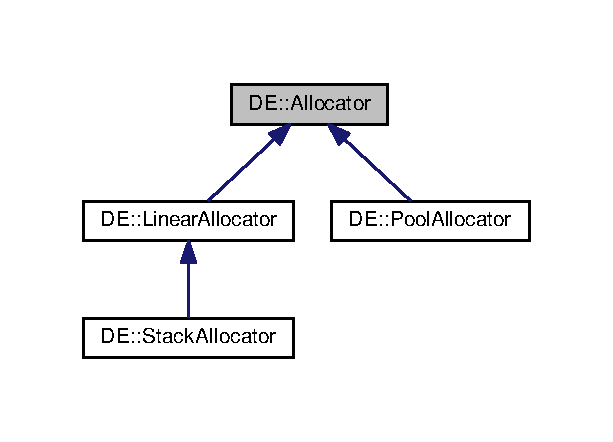
\includegraphics[width=294pt]{classDE_1_1Allocator__inherit__graph}
\end{center}
\end{figure}
\subsection*{Public Member Functions}
\begin{DoxyCompactItemize}
\item 
\hyperlink{classDE_1_1Allocator_ab6534df8f8e4c8b28ca129687bec3b26}{Allocator} ()\hypertarget{classDE_1_1Allocator_ab6534df8f8e4c8b28ca129687bec3b26}{}\label{classDE_1_1Allocator_ab6534df8f8e4c8b28ca129687bec3b26}

\begin{DoxyCompactList}\small\item\em Default Constructor. \end{DoxyCompactList}\item 
virtual \hyperlink{classDE_1_1Allocator_a8d95aa03ec7c7801d06a23f5f453961d}{$\sim$\+Allocator} ()\hypertarget{classDE_1_1Allocator_a8d95aa03ec7c7801d06a23f5f453961d}{}\label{classDE_1_1Allocator_a8d95aa03ec7c7801d06a23f5f453961d}

\begin{DoxyCompactList}\small\item\em Destructor. \end{DoxyCompactList}\item 
virtual u32 \hyperlink{classDE_1_1Allocator_af8e9d8df95e03bd2a5d2242d67c37ff2}{get\+Size} ()
\item 
virtual u32 \hyperlink{classDE_1_1Allocator_ab1cd017ccd297924b3afec3588f42848}{get\+Allocated} ()
\item 
virtual bool \hyperlink{classDE_1_1Allocator_a911a1c5749601a4950c0f88e828334df}{has\+Space} (u32 size)
\item 
virtual void \hyperlink{classDE_1_1Allocator_a4478c3fd1883e6d5fca88a479f0ccd12}{init} (u32 size)
\begin{DoxyCompactList}\small\item\em Constructor. \end{DoxyCompactList}\item 
virtual void \hyperlink{classDE_1_1Allocator_a3e89def629d55d2f6cdb0d0a4b9684f6}{init\+From\+Memory} (u32 size, void $\ast$mem)
\begin{DoxyCompactList}\small\item\em Constructor. \end{DoxyCompactList}\item 
virtual void $\ast$ \hyperlink{classDE_1_1Allocator_a25c66f6c09ca69ef083219fc7c2b0392}{allocate} (u32 size)=0
\begin{DoxyCompactList}\small\item\em Allocates memory. \end{DoxyCompactList}\item 
virtual void $\ast$ \hyperlink{classDE_1_1Allocator_ae8e197bc4bab60a9321b8c25596e927d}{allocate} (u32 size, u32 alignment)=0
\begin{DoxyCompactList}\small\item\em Allocates memory. \end{DoxyCompactList}\item 
virtual void \hyperlink{classDE_1_1Allocator_a9a01f5da5adafc6d5cee9b3e3e9859c4}{free} (const void $\ast$pointer)=0
\begin{DoxyCompactList}\small\item\em Frees memory. \end{DoxyCompactList}\item 
virtual void \hyperlink{classDE_1_1Allocator_a765f3ff9d6ff095bdfe4674652542a3d}{free\+Aligned} (const void $\ast$pointer)=0
\begin{DoxyCompactList}\small\item\em Frees aligned memory. \end{DoxyCompactList}\item 
virtual void \hyperlink{classDE_1_1Allocator_a0a08a7747d50ec63e6eaa1740f5de347}{reset} ()\hypertarget{classDE_1_1Allocator_a0a08a7747d50ec63e6eaa1740f5de347}{}\label{classDE_1_1Allocator_a0a08a7747d50ec63e6eaa1740f5de347}

\begin{DoxyCompactList}\small\item\em Frees aligned memory. \end{DoxyCompactList}\end{DoxyCompactItemize}
\subsection*{Protected Member Functions}
\begin{DoxyCompactItemize}
\item 
void {\bfseries check\+Allocate} (u32 size)\hypertarget{classDE_1_1Allocator_adfa4cc6e2a100ced016d76dad996ec03}{}\label{classDE_1_1Allocator_adfa4cc6e2a100ced016d76dad996ec03}

\item 
void {\bfseries check\+Free} ()\hypertarget{classDE_1_1Allocator_a77aa1061f03024b4908d1df48b5f6a9b}{}\label{classDE_1_1Allocator_a77aa1061f03024b4908d1df48b5f6a9b}

\item 
void {\bfseries set\+Allocated} (u32 size)\hypertarget{classDE_1_1Allocator_a1ba0de66726af5f264a32bbdc56e09e6}{}\label{classDE_1_1Allocator_a1ba0de66726af5f264a32bbdc56e09e6}

\item 
void {\bfseries \+\_\+init} (void $\ast$mem)\hypertarget{classDE_1_1Allocator_a26ac571c71cac6e35eaadef60b145d04}{}\label{classDE_1_1Allocator_a26ac571c71cac6e35eaadef60b145d04}

\end{DoxyCompactItemize}
\subsection*{Protected Attributes}
\begin{DoxyCompactItemize}
\item 
u32 {\bfseries m\+Total\+Size}\hypertarget{classDE_1_1Allocator_aceae0739788b604e09461cb87c9cee33}{}\label{classDE_1_1Allocator_aceae0739788b604e09461cb87c9cee33}

\item 
u32 {\bfseries m\+Allocated}\hypertarget{classDE_1_1Allocator_a5b5fdd9a1d11ae939f0dafee6aa65be7}{}\label{classDE_1_1Allocator_a5b5fdd9a1d11ae939f0dafee6aa65be7}

\item 
void $\ast$ {\bfseries m\+Start}\hypertarget{classDE_1_1Allocator_a4b8cbee3d0d9544e88ebdfaa62902b90}{}\label{classDE_1_1Allocator_a4b8cbee3d0d9544e88ebdfaa62902b90}

\item 
void $\ast$ {\bfseries m\+End}\hypertarget{classDE_1_1Allocator_adef4833178f44b6c047d47945d5c93d4}{}\label{classDE_1_1Allocator_adef4833178f44b6c047d47945d5c93d4}

\item 
void $\ast$ {\bfseries m\+Start\+Copy}\hypertarget{classDE_1_1Allocator_a26a25b124b6a727393ecaa51e8c9925b}{}\label{classDE_1_1Allocator_a26a25b124b6a727393ecaa51e8c9925b}

\end{DoxyCompactItemize}


\subsection{Detailed Description}
Manages memory allocation. 

\subsection{Member Function Documentation}
\index{D\+E\+::\+Allocator@{D\+E\+::\+Allocator}!allocate@{allocate}}
\index{allocate@{allocate}!D\+E\+::\+Allocator@{D\+E\+::\+Allocator}}
\subsubsection[{\texorpdfstring{allocate(u32 size)=0}{allocate(u32 size)=0}}]{\setlength{\rightskip}{0pt plus 5cm}virtual void$\ast$ D\+E\+::\+Allocator\+::allocate (
\begin{DoxyParamCaption}
\item[{u32}]{size}
\end{DoxyParamCaption}
)\hspace{0.3cm}{\ttfamily [pure virtual]}}\hypertarget{classDE_1_1Allocator_a25c66f6c09ca69ef083219fc7c2b0392}{}\label{classDE_1_1Allocator_a25c66f6c09ca69ef083219fc7c2b0392}


Allocates memory. 


\begin{DoxyParams}{Parameters}
{\em size} & Amount of memory you want to allocate. \\
\hline
\end{DoxyParams}
\begin{DoxyReturn}{Returns}
Pointer to memory chunk. 
\end{DoxyReturn}


Implemented in \hyperlink{classDE_1_1PoolAllocator_a55472e9fd8cbe6455706c781c1b1f2d9}{D\+E\+::\+Pool\+Allocator}, \hyperlink{classDE_1_1StackAllocator_a4b360ed983169d4063d0b85ac83ec156}{D\+E\+::\+Stack\+Allocator}, and \hyperlink{classDE_1_1LinearAllocator_a4758d08eb92d0a78a614d40822180ae4}{D\+E\+::\+Linear\+Allocator}.

\index{D\+E\+::\+Allocator@{D\+E\+::\+Allocator}!allocate@{allocate}}
\index{allocate@{allocate}!D\+E\+::\+Allocator@{D\+E\+::\+Allocator}}
\subsubsection[{\texorpdfstring{allocate(u32 size, u32 alignment)=0}{allocate(u32 size, u32 alignment)=0}}]{\setlength{\rightskip}{0pt plus 5cm}virtual void$\ast$ D\+E\+::\+Allocator\+::allocate (
\begin{DoxyParamCaption}
\item[{u32}]{size, }
\item[{u32}]{alignment}
\end{DoxyParamCaption}
)\hspace{0.3cm}{\ttfamily [pure virtual]}}\hypertarget{classDE_1_1Allocator_ae8e197bc4bab60a9321b8c25596e927d}{}\label{classDE_1_1Allocator_ae8e197bc4bab60a9321b8c25596e927d}


Allocates memory. 


\begin{DoxyParams}{Parameters}
{\em size} & Amount of memory you want to allocate. \\
\hline
{\em alignment} & Bytes alignment. \\
\hline
\end{DoxyParams}
\begin{DoxyReturn}{Returns}
Pointer to memory chunk. 
\end{DoxyReturn}


Implemented in \hyperlink{classDE_1_1PoolAllocator_a06a558e5d2b8a09b0a38ad8c6a4e100e}{D\+E\+::\+Pool\+Allocator}, \hyperlink{classDE_1_1StackAllocator_afa3e49ff8c47278c25e8ffcfa7897a80}{D\+E\+::\+Stack\+Allocator}, and \hyperlink{classDE_1_1LinearAllocator_ae5a5125718d29914d63e6dfece2deead}{D\+E\+::\+Linear\+Allocator}.

\index{D\+E\+::\+Allocator@{D\+E\+::\+Allocator}!free@{free}}
\index{free@{free}!D\+E\+::\+Allocator@{D\+E\+::\+Allocator}}
\subsubsection[{\texorpdfstring{free(const void $\ast$pointer)=0}{free(const void *pointer)=0}}]{\setlength{\rightskip}{0pt plus 5cm}virtual void D\+E\+::\+Allocator\+::free (
\begin{DoxyParamCaption}
\item[{const void $\ast$}]{pointer}
\end{DoxyParamCaption}
)\hspace{0.3cm}{\ttfamily [pure virtual]}}\hypertarget{classDE_1_1Allocator_a9a01f5da5adafc6d5cee9b3e3e9859c4}{}\label{classDE_1_1Allocator_a9a01f5da5adafc6d5cee9b3e3e9859c4}


Frees memory. 


\begin{DoxyParams}{Parameters}
{\em pointer} & Pointer to memory. \\
\hline
\end{DoxyParams}


Implemented in \hyperlink{classDE_1_1PoolAllocator_ac8566e6920e0f34f70c2f76758fbb68a}{D\+E\+::\+Pool\+Allocator}, \hyperlink{classDE_1_1StackAllocator_ae1c77f32df6421293da96dc322f33c98}{D\+E\+::\+Stack\+Allocator}, and \hyperlink{classDE_1_1LinearAllocator_ae1913dde9c2b91738d42686fb08cc755}{D\+E\+::\+Linear\+Allocator}.

\index{D\+E\+::\+Allocator@{D\+E\+::\+Allocator}!free\+Aligned@{free\+Aligned}}
\index{free\+Aligned@{free\+Aligned}!D\+E\+::\+Allocator@{D\+E\+::\+Allocator}}
\subsubsection[{\texorpdfstring{free\+Aligned(const void $\ast$pointer)=0}{freeAligned(const void *pointer)=0}}]{\setlength{\rightskip}{0pt plus 5cm}virtual void D\+E\+::\+Allocator\+::free\+Aligned (
\begin{DoxyParamCaption}
\item[{const void $\ast$}]{pointer}
\end{DoxyParamCaption}
)\hspace{0.3cm}{\ttfamily [pure virtual]}}\hypertarget{classDE_1_1Allocator_a765f3ff9d6ff095bdfe4674652542a3d}{}\label{classDE_1_1Allocator_a765f3ff9d6ff095bdfe4674652542a3d}


Frees aligned memory. 


\begin{DoxyParams}{Parameters}
{\em pointer} & Pointer to aligned memory. \\
\hline
\end{DoxyParams}


Implemented in \hyperlink{classDE_1_1PoolAllocator_af20c44a50efd12448f87b268e308fc92}{D\+E\+::\+Pool\+Allocator}, \hyperlink{classDE_1_1StackAllocator_aac3d433b63805fbd046a3ce70d6d6305}{D\+E\+::\+Stack\+Allocator}, and \hyperlink{classDE_1_1LinearAllocator_a4199d84edd3d515e0db8512efdf1f208}{D\+E\+::\+Linear\+Allocator}.

\index{D\+E\+::\+Allocator@{D\+E\+::\+Allocator}!get\+Allocated@{get\+Allocated}}
\index{get\+Allocated@{get\+Allocated}!D\+E\+::\+Allocator@{D\+E\+::\+Allocator}}
\subsubsection[{\texorpdfstring{get\+Allocated()}{getAllocated()}}]{\setlength{\rightskip}{0pt plus 5cm}u32 D\+E\+::\+Allocator\+::get\+Allocated (
\begin{DoxyParamCaption}
{}
\end{DoxyParamCaption}
)\hspace{0.3cm}{\ttfamily [virtual]}}\hypertarget{classDE_1_1Allocator_ab1cd017ccd297924b3afec3588f42848}{}\label{classDE_1_1Allocator_ab1cd017ccd297924b3afec3588f42848}
\begin{DoxyReturn}{Returns}
Amount of memory used. 
\end{DoxyReturn}
\index{D\+E\+::\+Allocator@{D\+E\+::\+Allocator}!get\+Size@{get\+Size}}
\index{get\+Size@{get\+Size}!D\+E\+::\+Allocator@{D\+E\+::\+Allocator}}
\subsubsection[{\texorpdfstring{get\+Size()}{getSize()}}]{\setlength{\rightskip}{0pt plus 5cm}u32 D\+E\+::\+Allocator\+::get\+Size (
\begin{DoxyParamCaption}
{}
\end{DoxyParamCaption}
)\hspace{0.3cm}{\ttfamily [virtual]}}\hypertarget{classDE_1_1Allocator_af8e9d8df95e03bd2a5d2242d67c37ff2}{}\label{classDE_1_1Allocator_af8e9d8df95e03bd2a5d2242d67c37ff2}
\begin{DoxyReturn}{Returns}
Total size. 
\end{DoxyReturn}
\index{D\+E\+::\+Allocator@{D\+E\+::\+Allocator}!has\+Space@{has\+Space}}
\index{has\+Space@{has\+Space}!D\+E\+::\+Allocator@{D\+E\+::\+Allocator}}
\subsubsection[{\texorpdfstring{has\+Space(u32 size)}{hasSpace(u32 size)}}]{\setlength{\rightskip}{0pt plus 5cm}bool D\+E\+::\+Allocator\+::has\+Space (
\begin{DoxyParamCaption}
\item[{u32}]{size}
\end{DoxyParamCaption}
)\hspace{0.3cm}{\ttfamily [virtual]}}\hypertarget{classDE_1_1Allocator_a911a1c5749601a4950c0f88e828334df}{}\label{classDE_1_1Allocator_a911a1c5749601a4950c0f88e828334df}
\begin{DoxyReturn}{Returns}
True if space is enough. 
\end{DoxyReturn}

\begin{DoxyParams}{Parameters}
{\em size} & Size you want to check. \\
\hline
\end{DoxyParams}
\index{D\+E\+::\+Allocator@{D\+E\+::\+Allocator}!init@{init}}
\index{init@{init}!D\+E\+::\+Allocator@{D\+E\+::\+Allocator}}
\subsubsection[{\texorpdfstring{init(u32 size)}{init(u32 size)}}]{\setlength{\rightskip}{0pt plus 5cm}void D\+E\+::\+Allocator\+::init (
\begin{DoxyParamCaption}
\item[{u32}]{size}
\end{DoxyParamCaption}
)\hspace{0.3cm}{\ttfamily [virtual]}}\hypertarget{classDE_1_1Allocator_a4478c3fd1883e6d5fca88a479f0ccd12}{}\label{classDE_1_1Allocator_a4478c3fd1883e6d5fca88a479f0ccd12}


Constructor. 


\begin{DoxyParams}{Parameters}
{\em size} & Amount of memory you want to allocate. \\
\hline
\end{DoxyParams}


Reimplemented in \hyperlink{classDE_1_1StackAllocator_a529ba39bd01e84cdb140db3343a7bf50}{D\+E\+::\+Stack\+Allocator}, and \hyperlink{classDE_1_1LinearAllocator_a70c826a33cfbedec4a93d5c3869b3655}{D\+E\+::\+Linear\+Allocator}.

\index{D\+E\+::\+Allocator@{D\+E\+::\+Allocator}!init\+From\+Memory@{init\+From\+Memory}}
\index{init\+From\+Memory@{init\+From\+Memory}!D\+E\+::\+Allocator@{D\+E\+::\+Allocator}}
\subsubsection[{\texorpdfstring{init\+From\+Memory(u32 size, void $\ast$mem)}{initFromMemory(u32 size, void *mem)}}]{\setlength{\rightskip}{0pt plus 5cm}void D\+E\+::\+Allocator\+::init\+From\+Memory (
\begin{DoxyParamCaption}
\item[{u32}]{size, }
\item[{void $\ast$}]{mem}
\end{DoxyParamCaption}
)\hspace{0.3cm}{\ttfamily [virtual]}}\hypertarget{classDE_1_1Allocator_a3e89def629d55d2f6cdb0d0a4b9684f6}{}\label{classDE_1_1Allocator_a3e89def629d55d2f6cdb0d0a4b9684f6}


Constructor. 


\begin{DoxyParams}{Parameters}
{\em size} & Amount of memory you want to allocate. \\
\hline
{\em mem} & Pointer to pre-\/allocated memory chunk. \\
\hline
\end{DoxyParams}


The documentation for this class was generated from the following files\+:\begin{DoxyCompactItemize}
\item 
include/\+Memory/Allocator.\+h\item 
source/\+Memory/Allocator.\+cpp\end{DoxyCompactItemize}

\hypertarget{classDE_1_1Array}{}\section{DE\+:\+:Array$<$ T $>$ Class Template Reference}
\label{classDE_1_1Array}\index{D\+E\+::\+Array$<$ T $>$@{D\+E\+::\+Array$<$ T $>$}}


\hyperlink{classDE_1_1Array}{Array} of elements. Fixed size.  




{\ttfamily \#include $<$Array.\+h$>$}



Inheritance diagram for DE\+:\+:Array$<$ T $>$\+:\nopagebreak
\begin{figure}[H]
\begin{center}
\leavevmode
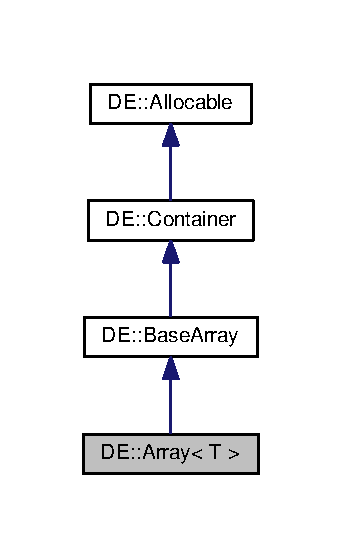
\includegraphics[width=164pt]{classDE_1_1Array__inherit__graph}
\end{center}
\end{figure}


Collaboration diagram for DE\+:\+:Array$<$ T $>$\+:\nopagebreak
\begin{figure}[H]
\begin{center}
\leavevmode
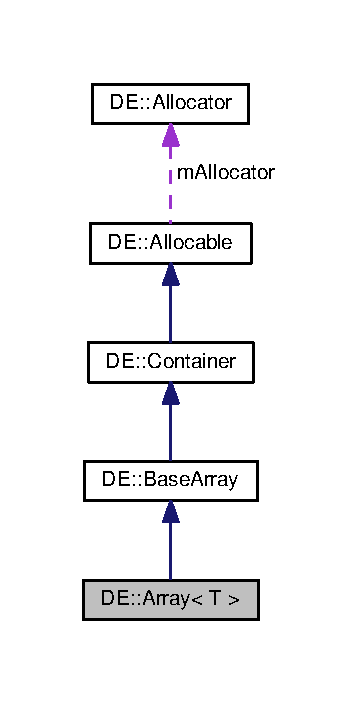
\includegraphics[width=172pt]{classDE_1_1Array__coll__graph}
\end{center}
\end{figure}
\subsection*{Public Member Functions}
\begin{DoxyCompactItemize}
\item 
\hyperlink{classDE_1_1Array_ada53b6c458d578ac3199a06ea3f258fb}{Array} ()\hypertarget{classDE_1_1Array_ada53b6c458d578ac3199a06ea3f258fb}{}\label{classDE_1_1Array_ada53b6c458d578ac3199a06ea3f258fb}

\begin{DoxyCompactList}\small\item\em Default Constructor. \end{DoxyCompactList}\item 
virtual \hyperlink{classDE_1_1Array_a3bcebef65959a0685e257308f50c58f2}{$\sim$\+Array} ()\hypertarget{classDE_1_1Array_a3bcebef65959a0685e257308f50c58f2}{}\label{classDE_1_1Array_a3bcebef65959a0685e257308f50c58f2}

\begin{DoxyCompactList}\small\item\em Destructor. \end{DoxyCompactList}\item 
void \hyperlink{classDE_1_1Array_a160b6d7bde381664d3a77c7bc72c7126}{init} (const \hyperlink{classDE_1_1Array}{Array}$<$ T $>$ \&other)
\begin{DoxyCompactList}\small\item\em Copy Constructor. \end{DoxyCompactList}\item 
void \hyperlink{classDE_1_1Array_a9e73e8109d4a8e1839c45f2443eb5f39}{fill} (T element)
\begin{DoxyCompactList}\small\item\em Fill the array with the same element. \end{DoxyCompactList}\item 
void \hyperlink{classDE_1_1Array_a9399e75853d0c2f946ad23ceeccf6309}{init} (const void $\ast$raw\+Array, const u32 length)
\begin{DoxyCompactList}\small\item\em Constructor from raw array. \end{DoxyCompactList}\item 
void \hyperlink{classDE_1_1Array_a424ca2b24f97dd2d0a23626b54405476}{init} (const void $\ast$raw\+Array, const u32 length, const u32 alignment)
\begin{DoxyCompactList}\small\item\em Constructor from raw array. Aligned. \end{DoxyCompactList}\item 
void \hyperlink{classDE_1_1Array_aca022d4ff92293f46a634260cb3fd9ed}{init} (const u32 length)
\begin{DoxyCompactList}\small\item\em Constructor. \end{DoxyCompactList}\item 
void \hyperlink{classDE_1_1Array_a5d03e54b2b7cc4b46b1c7c311f1b23c4}{init} (const u32 length, const u32 alignment)
\begin{DoxyCompactList}\small\item\em Constructor. Aligned. \end{DoxyCompactList}\item 
void \hyperlink{classDE_1_1Array_a2b0b137f752a2cf067359581e95bcd46}{put} (const \hyperlink{classDE_1_1Array}{Array}$<$ T $>$ \&other, u32 index)
\begin{DoxyCompactList}\small\item\em Copy an array into other. \end{DoxyCompactList}\item 
void \hyperlink{classDE_1_1Array_a612b948b4b8d915d223a89f4577bcabb}{put} (const void $\ast$raw\+Array, u32 index, const u32 length)
\begin{DoxyCompactList}\small\item\em Copy an array into other. \end{DoxyCompactList}\item 
T \& \hyperlink{classDE_1_1Array_a63fea3814adc4a5275b8564a568eddd3}{operator\mbox{[}$\,$\mbox{]}} (const size\+\_\+t i)
\begin{DoxyCompactList}\small\item\em Can be used for assignment. \end{DoxyCompactList}\end{DoxyCompactItemize}
\subsection*{Additional Inherited Members}


\subsection{Detailed Description}
\subsubsection*{template$<$class T$>$\\*
class D\+E\+::\+Array$<$ T $>$}

\hyperlink{classDE_1_1Array}{Array} of elements. Fixed size. 


\begin{DoxyTemplParams}{Template Parameters}
{\em Elements} & class. \\
\hline
\end{DoxyTemplParams}


\subsection{Member Function Documentation}
\index{D\+E\+::\+Array@{D\+E\+::\+Array}!fill@{fill}}
\index{fill@{fill}!D\+E\+::\+Array@{D\+E\+::\+Array}}
\subsubsection[{\texorpdfstring{fill(\+T element)}{fill(T element)}}]{\setlength{\rightskip}{0pt plus 5cm}template$<$class T$>$ void {\bf D\+E\+::\+Array}$<$ T $>$\+::fill (
\begin{DoxyParamCaption}
\item[{T}]{element}
\end{DoxyParamCaption}
)\hspace{0.3cm}{\ttfamily [inline]}}\hypertarget{classDE_1_1Array_a9e73e8109d4a8e1839c45f2443eb5f39}{}\label{classDE_1_1Array_a9e73e8109d4a8e1839c45f2443eb5f39}


Fill the array with the same element. 


\begin{DoxyParams}{Parameters}
{\em element} & The element. \\
\hline
\end{DoxyParams}
\index{D\+E\+::\+Array@{D\+E\+::\+Array}!init@{init}}
\index{init@{init}!D\+E\+::\+Array@{D\+E\+::\+Array}}
\subsubsection[{\texorpdfstring{init(const Array$<$ T $>$ \&other)}{init(const Array< T > &other)}}]{\setlength{\rightskip}{0pt plus 5cm}template$<$class T$>$ void {\bf D\+E\+::\+Array}$<$ T $>$\+::init (
\begin{DoxyParamCaption}
\item[{const {\bf Array}$<$ T $>$ \&}]{other}
\end{DoxyParamCaption}
)\hspace{0.3cm}{\ttfamily [inline]}}\hypertarget{classDE_1_1Array_a160b6d7bde381664d3a77c7bc72c7126}{}\label{classDE_1_1Array_a160b6d7bde381664d3a77c7bc72c7126}


Copy Constructor. 


\begin{DoxyParams}{Parameters}
{\em other} & Other \hyperlink{classDE_1_1Array}{Array}. \\
\hline
\end{DoxyParams}
\index{D\+E\+::\+Array@{D\+E\+::\+Array}!init@{init}}
\index{init@{init}!D\+E\+::\+Array@{D\+E\+::\+Array}}
\subsubsection[{\texorpdfstring{init(const void $\ast$raw\+Array, const u32 length)}{init(const void *rawArray, const u32 length)}}]{\setlength{\rightskip}{0pt plus 5cm}template$<$class T$>$ void {\bf D\+E\+::\+Array}$<$ T $>$\+::init (
\begin{DoxyParamCaption}
\item[{const void $\ast$}]{raw\+Array, }
\item[{const u32}]{length}
\end{DoxyParamCaption}
)\hspace{0.3cm}{\ttfamily [inline]}}\hypertarget{classDE_1_1Array_a9399e75853d0c2f946ad23ceeccf6309}{}\label{classDE_1_1Array_a9399e75853d0c2f946ad23ceeccf6309}


Constructor from raw array. 


\begin{DoxyParams}{Parameters}
{\em raw\+Array} & The raw array. \\
\hline
{\em length} & The length of the raw array. \\
\hline
\end{DoxyParams}
\index{D\+E\+::\+Array@{D\+E\+::\+Array}!init@{init}}
\index{init@{init}!D\+E\+::\+Array@{D\+E\+::\+Array}}
\subsubsection[{\texorpdfstring{init(const void $\ast$raw\+Array, const u32 length, const u32 alignment)}{init(const void *rawArray, const u32 length, const u32 alignment)}}]{\setlength{\rightskip}{0pt plus 5cm}template$<$class T$>$ void {\bf D\+E\+::\+Array}$<$ T $>$\+::init (
\begin{DoxyParamCaption}
\item[{const void $\ast$}]{raw\+Array, }
\item[{const u32}]{length, }
\item[{const u32}]{alignment}
\end{DoxyParamCaption}
)\hspace{0.3cm}{\ttfamily [inline]}}\hypertarget{classDE_1_1Array_a424ca2b24f97dd2d0a23626b54405476}{}\label{classDE_1_1Array_a424ca2b24f97dd2d0a23626b54405476}


Constructor from raw array. Aligned. 


\begin{DoxyParams}{Parameters}
{\em raw\+Array} & The raw array. \\
\hline
{\em length} & The length of the raw array. \\
\hline
{\em alignment} & Bytes alignment. \\
\hline
\end{DoxyParams}
\index{D\+E\+::\+Array@{D\+E\+::\+Array}!init@{init}}
\index{init@{init}!D\+E\+::\+Array@{D\+E\+::\+Array}}
\subsubsection[{\texorpdfstring{init(const u32 length)}{init(const u32 length)}}]{\setlength{\rightskip}{0pt plus 5cm}template$<$class T$>$ void {\bf D\+E\+::\+Array}$<$ T $>$\+::init (
\begin{DoxyParamCaption}
\item[{const u32}]{length}
\end{DoxyParamCaption}
)\hspace{0.3cm}{\ttfamily [inline]}}\hypertarget{classDE_1_1Array_aca022d4ff92293f46a634260cb3fd9ed}{}\label{classDE_1_1Array_aca022d4ff92293f46a634260cb3fd9ed}


Constructor. 


\begin{DoxyParams}{Parameters}
{\em length} & Length of the array. \\
\hline
\end{DoxyParams}
\index{D\+E\+::\+Array@{D\+E\+::\+Array}!init@{init}}
\index{init@{init}!D\+E\+::\+Array@{D\+E\+::\+Array}}
\subsubsection[{\texorpdfstring{init(const u32 length, const u32 alignment)}{init(const u32 length, const u32 alignment)}}]{\setlength{\rightskip}{0pt plus 5cm}template$<$class T$>$ void {\bf D\+E\+::\+Array}$<$ T $>$\+::init (
\begin{DoxyParamCaption}
\item[{const u32}]{length, }
\item[{const u32}]{alignment}
\end{DoxyParamCaption}
)\hspace{0.3cm}{\ttfamily [inline]}}\hypertarget{classDE_1_1Array_a5d03e54b2b7cc4b46b1c7c311f1b23c4}{}\label{classDE_1_1Array_a5d03e54b2b7cc4b46b1c7c311f1b23c4}


Constructor. Aligned. 


\begin{DoxyParams}{Parameters}
{\em length} & Length of the array. \\
\hline
{\em alignment} & Bytes alignment. \\
\hline
\end{DoxyParams}
\index{D\+E\+::\+Array@{D\+E\+::\+Array}!operator\mbox{[}$\,$\mbox{]}@{operator[]}}
\index{operator\mbox{[}$\,$\mbox{]}@{operator[]}!D\+E\+::\+Array@{D\+E\+::\+Array}}
\subsubsection[{\texorpdfstring{operator[](const size\+\_\+t i)}{operator[](const size_t i)}}]{\setlength{\rightskip}{0pt plus 5cm}template$<$class T$>$ T\& {\bf D\+E\+::\+Array}$<$ T $>$\+::operator\mbox{[}$\,$\mbox{]} (
\begin{DoxyParamCaption}
\item[{const size\+\_\+t}]{i}
\end{DoxyParamCaption}
)\hspace{0.3cm}{\ttfamily [inline]}}\hypertarget{classDE_1_1Array_a63fea3814adc4a5275b8564a568eddd3}{}\label{classDE_1_1Array_a63fea3814adc4a5275b8564a568eddd3}


Can be used for assignment. 


\begin{DoxyParams}{Parameters}
{\em i} & Index. \\
\hline
\end{DoxyParams}
\begin{DoxyReturn}{Returns}
Element reference. 
\end{DoxyReturn}
\index{D\+E\+::\+Array@{D\+E\+::\+Array}!put@{put}}
\index{put@{put}!D\+E\+::\+Array@{D\+E\+::\+Array}}
\subsubsection[{\texorpdfstring{put(const Array$<$ T $>$ \&other, u32 index)}{put(const Array< T > &other, u32 index)}}]{\setlength{\rightskip}{0pt plus 5cm}template$<$class T$>$ void {\bf D\+E\+::\+Array}$<$ T $>$\+::put (
\begin{DoxyParamCaption}
\item[{const {\bf Array}$<$ T $>$ \&}]{other, }
\item[{u32}]{index}
\end{DoxyParamCaption}
)\hspace{0.3cm}{\ttfamily [inline]}}\hypertarget{classDE_1_1Array_a2b0b137f752a2cf067359581e95bcd46}{}\label{classDE_1_1Array_a2b0b137f752a2cf067359581e95bcd46}


Copy an array into other. 


\begin{DoxyParams}{Parameters}
{\em other} & Other \hyperlink{classDE_1_1Array}{Array}. \\
\hline
{\em index} & Index (of the destiny array) from which to paste the other array. \\
\hline
\end{DoxyParams}
\index{D\+E\+::\+Array@{D\+E\+::\+Array}!put@{put}}
\index{put@{put}!D\+E\+::\+Array@{D\+E\+::\+Array}}
\subsubsection[{\texorpdfstring{put(const void $\ast$raw\+Array, u32 index, const u32 length)}{put(const void *rawArray, u32 index, const u32 length)}}]{\setlength{\rightskip}{0pt plus 5cm}template$<$class T$>$ void {\bf D\+E\+::\+Array}$<$ T $>$\+::put (
\begin{DoxyParamCaption}
\item[{const void $\ast$}]{raw\+Array, }
\item[{u32}]{index, }
\item[{const u32}]{length}
\end{DoxyParamCaption}
)\hspace{0.3cm}{\ttfamily [inline]}}\hypertarget{classDE_1_1Array_a612b948b4b8d915d223a89f4577bcabb}{}\label{classDE_1_1Array_a612b948b4b8d915d223a89f4577bcabb}


Copy an array into other. 


\begin{DoxyParams}{Parameters}
{\em other} & Other \hyperlink{classDE_1_1Array}{Array}. \\
\hline
{\em index} & Index (of the destiny array) from which to paste the other array. \\
\hline
{\em length} & Amount of element of the other array to be copied. \\
\hline
\end{DoxyParams}


The documentation for this class was generated from the following file\+:\begin{DoxyCompactItemize}
\item 
include/\+Containers/Array.\+h\end{DoxyCompactItemize}

\hypertarget{classDE_1_1BaseArray}{}\section{DE\+:\+:Base\+Array Class Reference}
\label{classDE_1_1BaseArray}\index{D\+E\+::\+Base\+Array@{D\+E\+::\+Base\+Array}}


Inheritance diagram for DE\+:\+:Base\+Array\+:
\nopagebreak
\begin{figure}[H]
\begin{center}
\leavevmode
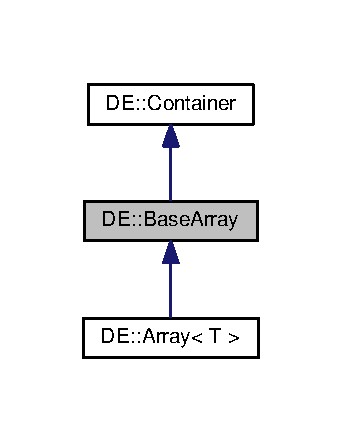
\includegraphics[width=164pt]{classDE_1_1BaseArray__inherit__graph}
\end{center}
\end{figure}


Collaboration diagram for DE\+:\+:Base\+Array\+:
\nopagebreak
\begin{figure}[H]
\begin{center}
\leavevmode
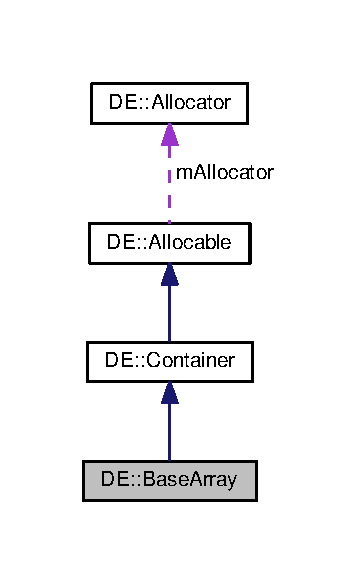
\includegraphics[width=172pt]{classDE_1_1BaseArray__coll__graph}
\end{center}
\end{figure}
\subsection*{Public Member Functions}
\begin{DoxyCompactItemize}
\item 
void {\bfseries set} (const void $\ast$raw\+Array)\hypertarget{classDE_1_1BaseArray_ac34bf7fbd622389f7f720f732eabd7be}{}\label{classDE_1_1BaseArray_ac34bf7fbd622389f7f720f732eabd7be}

\item 
void {\bfseries put} (const void $\ast$raw\+Array, u32 index, u32 length)\hypertarget{classDE_1_1BaseArray_ae064c6a309ec65f3dd3f4ece358c1fd0}{}\label{classDE_1_1BaseArray_ae064c6a309ec65f3dd3f4ece358c1fd0}

\end{DoxyCompactItemize}
\subsection*{Protected Member Functions}
\begin{DoxyCompactItemize}
\item 
void {\bfseries fill} (void $\ast$destiny, const void $\ast$source, u32 size)\hypertarget{classDE_1_1BaseArray_aa22f000b05b0b9e04f295f8e326dac6d}{}\label{classDE_1_1BaseArray_aa22f000b05b0b9e04f295f8e326dac6d}

\item 
void {\bfseries copy} (const \hyperlink{classDE_1_1BaseArray}{Base\+Array} \&other)\hypertarget{classDE_1_1BaseArray_ab8c75b509b9f9e5f86a9bd9f07f176d3}{}\label{classDE_1_1BaseArray_ab8c75b509b9f9e5f86a9bd9f07f176d3}

\item 
void {\bfseries init} (const void $\ast$raw\+Array, u32 length, u32 element\+Size)\hypertarget{classDE_1_1BaseArray_a02b09bebb65ea11f5c7b4b36a93745af}{}\label{classDE_1_1BaseArray_a02b09bebb65ea11f5c7b4b36a93745af}

\item 
void {\bfseries init} (const void $\ast$raw\+Array, u32 length, u32 element\+Size, u32 alignment)\hypertarget{classDE_1_1BaseArray_aa2769dac348aee44550c1a08d7374a2c}{}\label{classDE_1_1BaseArray_aa2769dac348aee44550c1a08d7374a2c}

\item 
void {\bfseries init} (u32 length, u32 element\+Size)\hypertarget{classDE_1_1BaseArray_a75c68b8c30583d8a14c0c433eee20749}{}\label{classDE_1_1BaseArray_a75c68b8c30583d8a14c0c433eee20749}

\item 
void {\bfseries init} (u32 length, u32 element\+Size, u32 alignment)\hypertarget{classDE_1_1BaseArray_a29b577dde57964102e4e5b358461ab73}{}\label{classDE_1_1BaseArray_a29b577dde57964102e4e5b358461ab73}

\item 
void {\bfseries allocate} (u32 length, u32 element\+Size, u32 alignment)\hypertarget{classDE_1_1BaseArray_a791cca1fbf420a3b24653800faa6fa80}{}\label{classDE_1_1BaseArray_a791cca1fbf420a3b24653800faa6fa80}

\end{DoxyCompactItemize}
\subsection*{Protected Attributes}
\begin{DoxyCompactItemize}
\item 
void $\ast$ {\bfseries m\+Start}\hypertarget{classDE_1_1BaseArray_a75351ce437cb954191bd17e6ca722a9c}{}\label{classDE_1_1BaseArray_a75351ce437cb954191bd17e6ca722a9c}

\end{DoxyCompactItemize}
\subsection*{Additional Inherited Members}


The documentation for this class was generated from the following files\+:\begin{DoxyCompactItemize}
\item 
include/\+Containers/Base\+Array.\+h\item 
source/\+Containers/Base\+Array.\+cpp\end{DoxyCompactItemize}

\hypertarget{classDE_1_1BaseList_1_1BaseIterator}{}\section{DE\+:\+:Base\+List\+:\+:Base\+Iterator Class Reference}
\label{classDE_1_1BaseList_1_1BaseIterator}\index{D\+E\+::\+Base\+List\+::\+Base\+Iterator@{D\+E\+::\+Base\+List\+::\+Base\+Iterator}}
\subsection*{Public Member Functions}
\begin{DoxyCompactItemize}
\item 
{\bfseries Base\+Iterator} (const \hyperlink{classDE_1_1BaseList_1_1BaseIterator}{Base\+Iterator} \&other)\hypertarget{classDE_1_1BaseList_1_1BaseIterator_ac721c46b8e92ab27a2276009ae9b4958}{}\label{classDE_1_1BaseList_1_1BaseIterator_ac721c46b8e92ab27a2276009ae9b4958}

\item 
void {\bfseries init} (\hyperlink{classDE_1_1BaseList_1_1BaseNode}{Base\+Node} $\ast$start)\hypertarget{classDE_1_1BaseList_1_1BaseIterator_a66520bed5f88fbde92bfdb8bae963853}{}\label{classDE_1_1BaseList_1_1BaseIterator_a66520bed5f88fbde92bfdb8bae963853}

\item 
bool {\bfseries is\+Null} ()\hypertarget{classDE_1_1BaseList_1_1BaseIterator_a8d8d7cdb1fbe7f3f83f050dfe0be8b5c}{}\label{classDE_1_1BaseList_1_1BaseIterator_a8d8d7cdb1fbe7f3f83f050dfe0be8b5c}

\item 
bool {\bfseries has\+Next} ()\hypertarget{classDE_1_1BaseList_1_1BaseIterator_ab66f470e91d4f6240f9b47455f5b9515}{}\label{classDE_1_1BaseList_1_1BaseIterator_ab66f470e91d4f6240f9b47455f5b9515}

\item 
void {\bfseries next} ()\hypertarget{classDE_1_1BaseList_1_1BaseIterator_a14c54397d923df4866faf093e3921dc9}{}\label{classDE_1_1BaseList_1_1BaseIterator_a14c54397d923df4866faf093e3921dc9}

\item 
\hyperlink{classDE_1_1BaseList_1_1BaseIterator}{Base\+Iterator} {\bfseries get\+Next} ()\hypertarget{classDE_1_1BaseList_1_1BaseIterator_aa0c954b78cea1c33c5dd92ff02b7391f}{}\label{classDE_1_1BaseList_1_1BaseIterator_aa0c954b78cea1c33c5dd92ff02b7391f}

\item 
bool {\bfseries has\+Prev} ()\hypertarget{classDE_1_1BaseList_1_1BaseIterator_a6b288184084bb6c601eca349c44bdfa1}{}\label{classDE_1_1BaseList_1_1BaseIterator_a6b288184084bb6c601eca349c44bdfa1}

\item 
void {\bfseries prev} ()\hypertarget{classDE_1_1BaseList_1_1BaseIterator_a95390486c0274de6e5d5339d29fd9f41}{}\label{classDE_1_1BaseList_1_1BaseIterator_a95390486c0274de6e5d5339d29fd9f41}

\item 
\hyperlink{classDE_1_1BaseList_1_1BaseIterator}{Base\+Iterator} {\bfseries get\+Prev} ()\hypertarget{classDE_1_1BaseList_1_1BaseIterator_ab3fd7fc65c180a260915ac5f40c852a4}{}\label{classDE_1_1BaseList_1_1BaseIterator_ab3fd7fc65c180a260915ac5f40c852a4}

\item 
void $\ast$ {\bfseries get} ()\hypertarget{classDE_1_1BaseList_1_1BaseIterator_acb122cfbb3103c72dfd216e4362f985d}{}\label{classDE_1_1BaseList_1_1BaseIterator_acb122cfbb3103c72dfd216e4362f985d}

\item 
void {\bfseries set} (void $\ast$element)\hypertarget{classDE_1_1BaseList_1_1BaseIterator_a96a3c5dd1acaaea211a7185c5dede60d}{}\label{classDE_1_1BaseList_1_1BaseIterator_a96a3c5dd1acaaea211a7185c5dede60d}

\item 
bool {\bfseries is\+Reverse} ()\hypertarget{classDE_1_1BaseList_1_1BaseIterator_a18baaa6b5bf724aadc953502dadb8f13}{}\label{classDE_1_1BaseList_1_1BaseIterator_a18baaa6b5bf724aadc953502dadb8f13}

\item 
void {\bfseries set\+Reverse} (bool is\+Reverse)\hypertarget{classDE_1_1BaseList_1_1BaseIterator_accb2d241b433cde68cead38ff597bf92}{}\label{classDE_1_1BaseList_1_1BaseIterator_accb2d241b433cde68cead38ff597bf92}

\item 
bool {\bfseries operator==} (const \hyperlink{classDE_1_1BaseList_1_1BaseIterator}{Base\+Iterator} \&rhs) const \hypertarget{classDE_1_1BaseList_1_1BaseIterator_a3bc3db8e37e932f9bac170b3153bf72e}{}\label{classDE_1_1BaseList_1_1BaseIterator_a3bc3db8e37e932f9bac170b3153bf72e}

\item 
bool {\bfseries operator!=} (const \hyperlink{classDE_1_1BaseList_1_1BaseIterator}{Base\+Iterator} \&rhs) const \hypertarget{classDE_1_1BaseList_1_1BaseIterator_a0a3ac2417dc8da014d919698d0197836}{}\label{classDE_1_1BaseList_1_1BaseIterator_a0a3ac2417dc8da014d919698d0197836}

\item 
\hyperlink{classDE_1_1BaseList_1_1BaseIterator}{Base\+Iterator} \& {\bfseries operator=} (const \hyperlink{classDE_1_1BaseList_1_1BaseIterator}{Base\+Iterator} \&rhs)\hypertarget{classDE_1_1BaseList_1_1BaseIterator_aa9b056ea76d74bb8fe855fe9b167b065}{}\label{classDE_1_1BaseList_1_1BaseIterator_aa9b056ea76d74bb8fe855fe9b167b065}

\end{DoxyCompactItemize}
\subsection*{Friends}
\begin{DoxyCompactItemize}
\item 
class {\bfseries Base\+List}\hypertarget{classDE_1_1BaseList_1_1BaseIterator_a6870f07ae8ce7c407b1572cae9417274}{}\label{classDE_1_1BaseList_1_1BaseIterator_a6870f07ae8ce7c407b1572cae9417274}

\end{DoxyCompactItemize}


The documentation for this class was generated from the following files\+:\begin{DoxyCompactItemize}
\item 
include/\+Containers/Base\+List.\+h\item 
source/\+Containers/Base\+List.\+cpp\end{DoxyCompactItemize}

\hypertarget{classDE_1_1BaseList}{}\section{DE\+:\+:Base\+List Class Reference}
\label{classDE_1_1BaseList}\index{D\+E\+::\+Base\+List@{D\+E\+::\+Base\+List}}


Inheritance diagram for DE\+:\+:Base\+List\+:
\nopagebreak
\begin{figure}[H]
\begin{center}
\leavevmode
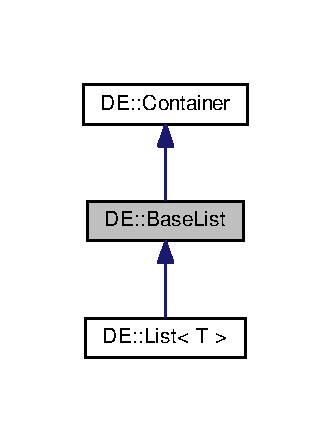
\includegraphics[width=159pt]{classDE_1_1BaseList__inherit__graph}
\end{center}
\end{figure}


Collaboration diagram for DE\+:\+:Base\+List\+:
\nopagebreak
\begin{figure}[H]
\begin{center}
\leavevmode
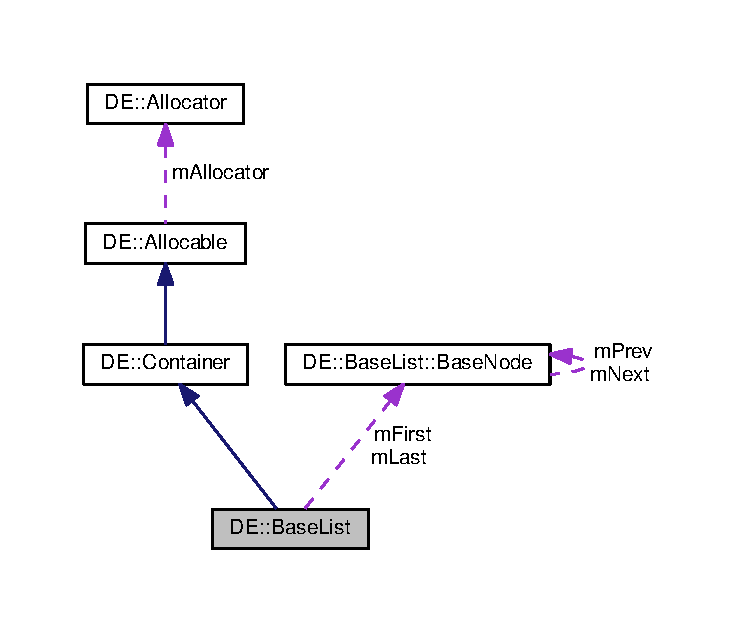
\includegraphics[width=350pt]{classDE_1_1BaseList__coll__graph}
\end{center}
\end{figure}
\subsection*{Classes}
\begin{DoxyCompactItemize}
\item 
class \hyperlink{classDE_1_1BaseList_1_1BaseIterator}{Base\+Iterator}
\item 
class \hyperlink{classDE_1_1BaseList_1_1BaseNode}{Base\+Node}
\end{DoxyCompactItemize}
\subsection*{Public Member Functions}
\begin{DoxyCompactItemize}
\item 
void {\bfseries clear} ()\hypertarget{classDE_1_1BaseList_a1fb264de58ba818c65da7623e2d42343}{}\label{classDE_1_1BaseList_a1fb264de58ba818c65da7623e2d42343}

\end{DoxyCompactItemize}
\subsection*{Static Public Member Functions}
\begin{DoxyCompactItemize}
\item 
static const u32 \& {\bfseries get\+Node\+Size} ()\hypertarget{classDE_1_1BaseList_a022bd54e1b6af0b10d352989fc9adc34}{}\label{classDE_1_1BaseList_a022bd54e1b6af0b10d352989fc9adc34}

\end{DoxyCompactItemize}
\subsection*{Protected Member Functions}
\begin{DoxyCompactItemize}
\item 
void {\bfseries allocate} (u32 element\+Size, u32 alignment)\hypertarget{classDE_1_1BaseList_a1af33f5611e6672bfba3a759004fa80e}{}\label{classDE_1_1BaseList_a1af33f5611e6672bfba3a759004fa80e}

\item 
void {\bfseries copy} (const \hyperlink{classDE_1_1BaseList}{Base\+List} \&other)\hypertarget{classDE_1_1BaseList_a3c678d1a2f536c642abe5a7dd800cc79}{}\label{classDE_1_1BaseList_a3c678d1a2f536c642abe5a7dd800cc79}

\item 
void {\bfseries init} (u32 element\+Size)\hypertarget{classDE_1_1BaseList_af61aef7cba6bac35ea183e0f33f114fa}{}\label{classDE_1_1BaseList_af61aef7cba6bac35ea183e0f33f114fa}

\item 
\hyperlink{classDE_1_1BaseList_1_1BaseIterator}{Base\+Iterator} {\bfseries get\+Iterator} () const \hypertarget{classDE_1_1BaseList_ad3f52d9aeab85bad232394ad0809cc40}{}\label{classDE_1_1BaseList_ad3f52d9aeab85bad232394ad0809cc40}

\item 
\hyperlink{classDE_1_1BaseList_1_1BaseIterator}{Base\+Iterator} {\bfseries get\+Rev\+Iterator} () const \hypertarget{classDE_1_1BaseList_a41028ea5b53c8f9229d2b0e127fbbb9c}{}\label{classDE_1_1BaseList_a41028ea5b53c8f9229d2b0e127fbbb9c}

\item 
\hyperlink{classDE_1_1BaseList_1_1BaseIterator}{Base\+Iterator} {\bfseries get\+First} () const \hypertarget{classDE_1_1BaseList_a9cdf4d25a7e575ca5e8398c6c58ddb18}{}\label{classDE_1_1BaseList_a9cdf4d25a7e575ca5e8398c6c58ddb18}

\item 
\hyperlink{classDE_1_1BaseList_1_1BaseIterator}{Base\+Iterator} {\bfseries get\+Last} () const \hypertarget{classDE_1_1BaseList_af797b5d09fab2c05ca9cab7bb7f1db32}{}\label{classDE_1_1BaseList_af797b5d09fab2c05ca9cab7bb7f1db32}

\item 
bool {\bfseries is\+Empty} () const \hypertarget{classDE_1_1BaseList_aad916f630075cf2df2501e98ebfa23de}{}\label{classDE_1_1BaseList_aad916f630075cf2df2501e98ebfa23de}

\item 
void {\bfseries push\+Front} (void $\ast$element)\hypertarget{classDE_1_1BaseList_a5e6869690713975deafa0e055c977da0}{}\label{classDE_1_1BaseList_a5e6869690713975deafa0e055c977da0}

\item 
void {\bfseries push\+Back} (void $\ast$element)\hypertarget{classDE_1_1BaseList_a0178a7d3ce60727d0dc908e92479a5e0}{}\label{classDE_1_1BaseList_a0178a7d3ce60727d0dc908e92479a5e0}

\item 
void $\ast$ {\bfseries pop\+Front} ()\hypertarget{classDE_1_1BaseList_a3910c757374eee205c5e4fe66fa5b443}{}\label{classDE_1_1BaseList_a3910c757374eee205c5e4fe66fa5b443}

\item 
void $\ast$ {\bfseries pop\+Back} ()\hypertarget{classDE_1_1BaseList_a9db5355ad9a1e6ae10c1e179a7e816e6}{}\label{classDE_1_1BaseList_a9db5355ad9a1e6ae10c1e179a7e816e6}

\item 
void $\ast$ {\bfseries get} (u32 index) const \hypertarget{classDE_1_1BaseList_a8431d5d521a3620fea45c20da0d8e4b3}{}\label{classDE_1_1BaseList_a8431d5d521a3620fea45c20da0d8e4b3}

\item 
void {\bfseries set} (u32 index, void $\ast$element)\hypertarget{classDE_1_1BaseList_add70f7c86284bf46795159ca2ac49960}{}\label{classDE_1_1BaseList_add70f7c86284bf46795159ca2ac49960}

\item 
void {\bfseries swap} (u32 index1, u32 index2)\hypertarget{classDE_1_1BaseList_a9bcf75745e1644fd87a12e439afc5c9c}{}\label{classDE_1_1BaseList_a9bcf75745e1644fd87a12e439afc5c9c}

\item 
void {\bfseries remove} (u32 index)\hypertarget{classDE_1_1BaseList_ae15c3960b5603ca12e1e6560bb922b6a}{}\label{classDE_1_1BaseList_ae15c3960b5603ca12e1e6560bb922b6a}

\item 
void {\bfseries remove} (\hyperlink{classDE_1_1BaseList_1_1BaseIterator}{Base\+Iterator} \&it)\hypertarget{classDE_1_1BaseList_ad89a50036ae9fcffa04d9dd3ed4de5b8}{}\label{classDE_1_1BaseList_ad89a50036ae9fcffa04d9dd3ed4de5b8}

\item 
void {\bfseries insert} (u32 index, void $\ast$element)\hypertarget{classDE_1_1BaseList_a84bd701e006411b4c30bd482c3c48a81}{}\label{classDE_1_1BaseList_a84bd701e006411b4c30bd482c3c48a81}

\item 
void {\bfseries insert} (\hyperlink{classDE_1_1BaseList_1_1BaseIterator}{Base\+Iterator} \&it, void $\ast$element)\hypertarget{classDE_1_1BaseList_a74dc509dbca3bca1ff7bb420d249a556}{}\label{classDE_1_1BaseList_a74dc509dbca3bca1ff7bb420d249a556}

\end{DoxyCompactItemize}
\subsection*{Protected Attributes}
\begin{DoxyCompactItemize}
\item 
\hyperlink{classDE_1_1BaseList_1_1BaseNode}{Base\+Node} $\ast$ {\bfseries m\+First}\hypertarget{classDE_1_1BaseList_ac5593890d21a73cfa4c837f87b5db5b1}{}\label{classDE_1_1BaseList_ac5593890d21a73cfa4c837f87b5db5b1}

\item 
\hyperlink{classDE_1_1BaseList_1_1BaseNode}{Base\+Node} $\ast$ {\bfseries m\+Last}\hypertarget{classDE_1_1BaseList_a757f5ad3193919dd4e81f259e07b07af}{}\label{classDE_1_1BaseList_a757f5ad3193919dd4e81f259e07b07af}

\end{DoxyCompactItemize}
\subsection*{Friends}
\begin{DoxyCompactItemize}
\item 
class {\bfseries Base\+Iterator}\hypertarget{classDE_1_1BaseList_a95d719a456031e0a03c45a657435f35b}{}\label{classDE_1_1BaseList_a95d719a456031e0a03c45a657435f35b}

\end{DoxyCompactItemize}


The documentation for this class was generated from the following files\+:\begin{DoxyCompactItemize}
\item 
include/\+Containers/Base\+List.\+h\item 
source/\+Containers/Base\+List.\+cpp\end{DoxyCompactItemize}

\hypertarget{classDE_1_1BaseList_1_1BaseNode}{}\section{DE\+:\+:Base\+List\+:\+:Base\+Node Class Reference}
\label{classDE_1_1BaseList_1_1BaseNode}\index{D\+E\+::\+Base\+List\+::\+Base\+Node@{D\+E\+::\+Base\+List\+::\+Base\+Node}}


Collaboration diagram for DE\+:\+:Base\+List\+:\+:Base\+Node\+:\nopagebreak
\begin{figure}[H]
\begin{center}
\leavevmode
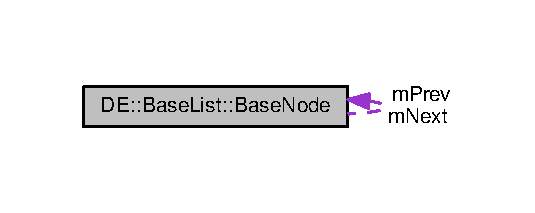
\includegraphics[width=257pt]{classDE_1_1BaseList_1_1BaseNode__coll__graph}
\end{center}
\end{figure}
\subsection*{Public Member Functions}
\begin{DoxyCompactItemize}
\item 
void {\bfseries init} ()\hypertarget{classDE_1_1BaseList_1_1BaseNode_abf2670b2c8a2be2da32f1c3311b8fe5c}{}\label{classDE_1_1BaseList_1_1BaseNode_abf2670b2c8a2be2da32f1c3311b8fe5c}

\item 
void {\bfseries init} (void $\ast$element)\hypertarget{classDE_1_1BaseList_1_1BaseNode_a54541a1cc63b48a4f5ebad2a279718e4}{}\label{classDE_1_1BaseList_1_1BaseNode_a54541a1cc63b48a4f5ebad2a279718e4}

\end{DoxyCompactItemize}
\subsection*{Public Attributes}
\begin{DoxyCompactItemize}
\item 
\hyperlink{classDE_1_1BaseList_1_1BaseNode}{Base\+Node} $\ast$ {\bfseries m\+Next}\hypertarget{classDE_1_1BaseList_1_1BaseNode_a888ef5f6584191fa6d92e9dc1df52c2c}{}\label{classDE_1_1BaseList_1_1BaseNode_a888ef5f6584191fa6d92e9dc1df52c2c}

\item 
\hyperlink{classDE_1_1BaseList_1_1BaseNode}{Base\+Node} $\ast$ {\bfseries m\+Prev}\hypertarget{classDE_1_1BaseList_1_1BaseNode_a94243487fddf9c0f9929fd556da89c61}{}\label{classDE_1_1BaseList_1_1BaseNode_a94243487fddf9c0f9929fd556da89c61}

\item 
void $\ast$ {\bfseries m\+Element}\hypertarget{classDE_1_1BaseList_1_1BaseNode_a8da52c072df5d392289e388f7dd32650}{}\label{classDE_1_1BaseList_1_1BaseNode_a8da52c072df5d392289e388f7dd32650}

\end{DoxyCompactItemize}


The documentation for this class was generated from the following files\+:\begin{DoxyCompactItemize}
\item 
include/\+Containers/Base\+List.\+h\item 
source/\+Containers/Base\+List.\+cpp\end{DoxyCompactItemize}

\hypertarget{classDE_1_1Container}{}\section{DE\+:\+:Container Class Reference}
\label{classDE_1_1Container}\index{D\+E\+::\+Container@{D\+E\+::\+Container}}


Inheritance diagram for DE\+:\+:Container\+:\nopagebreak
\begin{figure}[H]
\begin{center}
\leavevmode
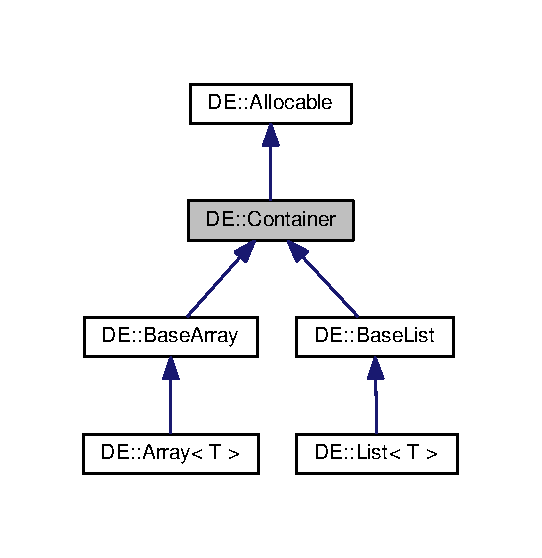
\includegraphics[width=260pt]{classDE_1_1Container__inherit__graph}
\end{center}
\end{figure}


Collaboration diagram for DE\+:\+:Container\+:\nopagebreak
\begin{figure}[H]
\begin{center}
\leavevmode
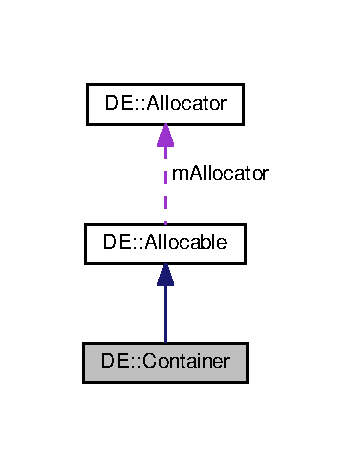
\includegraphics[width=170pt]{classDE_1_1Container__coll__graph}
\end{center}
\end{figure}
\subsection*{Public Member Functions}
\begin{DoxyCompactItemize}
\item 
u32 {\bfseries get\+Length} () const \hypertarget{classDE_1_1Container_ac4e1b4aefaecda0e225312fe463c9995}{}\label{classDE_1_1Container_ac4e1b4aefaecda0e225312fe463c9995}

\end{DoxyCompactItemize}
\subsection*{Protected Member Functions}
\begin{DoxyCompactItemize}
\item 
void {\bfseries init} (const u32 length, const u32 element\+Size, const u32 alignment)\hypertarget{classDE_1_1Container_a449de30288ea53726ece6268becc9d86}{}\label{classDE_1_1Container_a449de30288ea53726ece6268becc9d86}

\end{DoxyCompactItemize}
\subsection*{Protected Attributes}
\begin{DoxyCompactItemize}
\item 
u32 {\bfseries m\+Element\+Size}\hypertarget{classDE_1_1Container_aa644444a2ab6f47a2f23a24fc3735022}{}\label{classDE_1_1Container_aa644444a2ab6f47a2f23a24fc3735022}

\item 
u32 {\bfseries m\+Length}\hypertarget{classDE_1_1Container_acde96d5b0bd1bd51c64b762b77b81fbb}{}\label{classDE_1_1Container_acde96d5b0bd1bd51c64b762b77b81fbb}

\item 
u32 {\bfseries m\+Alignment}\hypertarget{classDE_1_1Container_af34003e0c91ad31e4d744d3b9f4bb7c1}{}\label{classDE_1_1Container_af34003e0c91ad31e4d744d3b9f4bb7c1}

\end{DoxyCompactItemize}
\subsection*{Additional Inherited Members}


The documentation for this class was generated from the following files\+:\begin{DoxyCompactItemize}
\item 
include/\+Containers/Container.\+h\item 
source/\+Containers/Container.\+cpp\end{DoxyCompactItemize}

\hypertarget{classDE_1_1List_1_1Iterator}{}\section{DE\+:\+:List$<$ T $>$\+:\+:Iterator Class Reference}
\label{classDE_1_1List_1_1Iterator}\index{D\+E\+::\+List$<$ T $>$\+::\+Iterator@{D\+E\+::\+List$<$ T $>$\+::\+Iterator}}


Inheritance diagram for DE\+:\+:List$<$ T $>$\+:\+:Iterator\+:\nopagebreak
\begin{figure}[H]
\begin{center}
\leavevmode
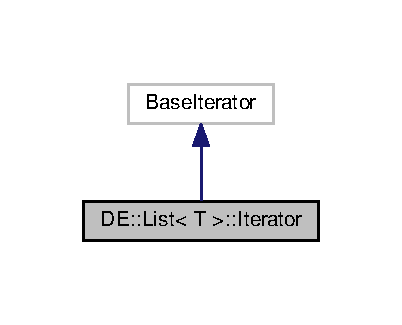
\includegraphics[width=193pt]{classDE_1_1List_1_1Iterator__inherit__graph}
\end{center}
\end{figure}


Collaboration diagram for DE\+:\+:List$<$ T $>$\+:\+:Iterator\+:\nopagebreak
\begin{figure}[H]
\begin{center}
\leavevmode
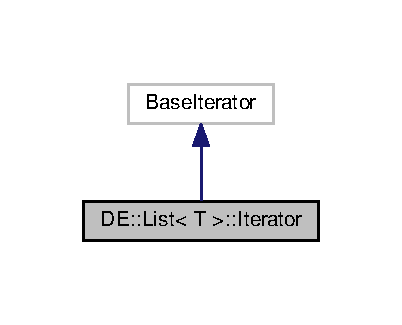
\includegraphics[width=193pt]{classDE_1_1List_1_1Iterator__coll__graph}
\end{center}
\end{figure}
\subsection*{Public Member Functions}
\begin{DoxyCompactItemize}
\item 
{\bfseries Iterator} (const Base\+Iterator \&other)\hypertarget{classDE_1_1List_1_1Iterator_aec3de14e44866dc96439a44e484756bd}{}\label{classDE_1_1List_1_1Iterator_aec3de14e44866dc96439a44e484756bd}

\item 
virtual T \& {\bfseries get} ()\hypertarget{classDE_1_1List_1_1Iterator_a4e83d04d4bc5e7715cf8535be70f8796}{}\label{classDE_1_1List_1_1Iterator_a4e83d04d4bc5e7715cf8535be70f8796}

\item 
virtual void {\bfseries set} (T \&element)\hypertarget{classDE_1_1List_1_1Iterator_a76effe78048f7c8b0b7b7cc9e24044be}{}\label{classDE_1_1List_1_1Iterator_a76effe78048f7c8b0b7b7cc9e24044be}

\item 
\hyperlink{classDE_1_1List_1_1Iterator}{Iterator} {\bfseries get\+Next} ()\hypertarget{classDE_1_1List_1_1Iterator_ae74a3fdd51d427c989adee0fbe218c3c}{}\label{classDE_1_1List_1_1Iterator_ae74a3fdd51d427c989adee0fbe218c3c}

\item 
\hyperlink{classDE_1_1List_1_1Iterator}{Iterator} {\bfseries get\+Prev} ()\hypertarget{classDE_1_1List_1_1Iterator_a335fea104b4908acad300498de017156}{}\label{classDE_1_1List_1_1Iterator_a335fea104b4908acad300498de017156}

\end{DoxyCompactItemize}


The documentation for this class was generated from the following file\+:\begin{DoxyCompactItemize}
\item 
include/\+Containers/List.\+h\end{DoxyCompactItemize}

\hypertarget{classDE_1_1LinearAllocator}{}\section{DE\+:\+:Linear\+Allocator Class Reference}
\label{classDE_1_1LinearAllocator}\index{D\+E\+::\+Linear\+Allocator@{D\+E\+::\+Linear\+Allocator}}


Allocates memory in a linear way. The whole memory is freed in one shot.  




{\ttfamily \#include $<$Linear\+Allocator.\+h$>$}



Inheritance diagram for DE\+:\+:Linear\+Allocator\+:
\nopagebreak
\begin{figure}[H]
\begin{center}
\leavevmode
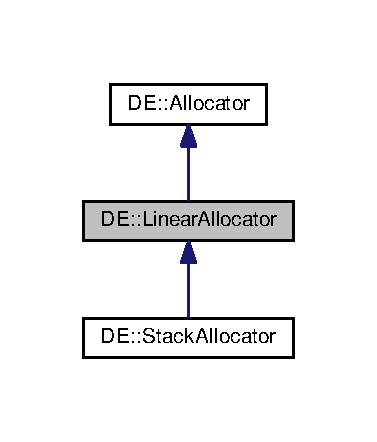
\includegraphics[width=181pt]{classDE_1_1LinearAllocator__inherit__graph}
\end{center}
\end{figure}


Collaboration diagram for DE\+:\+:Linear\+Allocator\+:\nopagebreak
\begin{figure}[H]
\begin{center}
\leavevmode
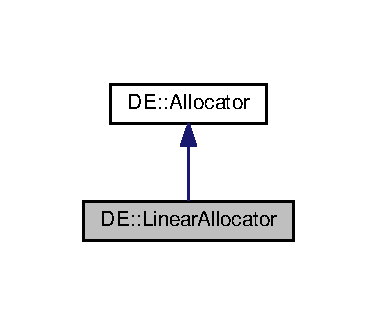
\includegraphics[width=181pt]{classDE_1_1LinearAllocator__coll__graph}
\end{center}
\end{figure}
\subsection*{Public Member Functions}
\begin{DoxyCompactItemize}
\item 
\hyperlink{classDE_1_1LinearAllocator_a39842c06f25b2eab2dd5ea4a204ad047}{Linear\+Allocator} ()\hypertarget{classDE_1_1LinearAllocator_a39842c06f25b2eab2dd5ea4a204ad047}{}\label{classDE_1_1LinearAllocator_a39842c06f25b2eab2dd5ea4a204ad047}

\begin{DoxyCompactList}\small\item\em Default Constructor. \end{DoxyCompactList}\item 
virtual \hyperlink{classDE_1_1LinearAllocator_a4ee6390f3ad8b726c142db0486d60fe2}{$\sim$\+Linear\+Allocator} ()\hypertarget{classDE_1_1LinearAllocator_a4ee6390f3ad8b726c142db0486d60fe2}{}\label{classDE_1_1LinearAllocator_a4ee6390f3ad8b726c142db0486d60fe2}

\begin{DoxyCompactList}\small\item\em Destructor. \end{DoxyCompactList}\item 
void \hyperlink{classDE_1_1LinearAllocator_aee64419a4f3c40ac5163ebb744a55155}{set\+Reverse} (bool is\+Reverse)
\begin{DoxyCompactList}\small\item\em Sets the direction of allocation. \end{DoxyCompactList}\item 
virtual void \hyperlink{classDE_1_1LinearAllocator_afc065d6a36571958cb33648894fb6c57}{init} (const u32 size)
\begin{DoxyCompactList}\small\item\em Constructor. \end{DoxyCompactList}\item 
virtual void $\ast$ \hyperlink{classDE_1_1LinearAllocator_a6d037588499a66590b52335c8b221454}{allocate} (const u32 size)
\begin{DoxyCompactList}\small\item\em Allocates memory. \end{DoxyCompactList}\item 
virtual void $\ast$ \hyperlink{classDE_1_1LinearAllocator_a5d6bf7e2dfe65f6795e77b3a2ed9e811}{allocate} (const u32 size, const u32 alignment)
\begin{DoxyCompactList}\small\item\em Allocates memory. \end{DoxyCompactList}\item 
virtual void \hyperlink{classDE_1_1LinearAllocator_ae1913dde9c2b91738d42686fb08cc755}{free} (const void $\ast$pointer)
\begin{DoxyCompactList}\small\item\em Frees memory. \end{DoxyCompactList}\item 
virtual void \hyperlink{classDE_1_1LinearAllocator_a4199d84edd3d515e0db8512efdf1f208}{free\+Aligned} (const void $\ast$pointer)
\begin{DoxyCompactList}\small\item\em Frees aligned memory. \end{DoxyCompactList}\item 
virtual void \hyperlink{classDE_1_1LinearAllocator_a0dbec6e2529dc2f13757c104b17bbdda}{reset} ()\hypertarget{classDE_1_1LinearAllocator_a0dbec6e2529dc2f13757c104b17bbdda}{}\label{classDE_1_1LinearAllocator_a0dbec6e2529dc2f13757c104b17bbdda}

\begin{DoxyCompactList}\small\item\em Frees aligned memory. \end{DoxyCompactList}\end{DoxyCompactItemize}
\subsection*{Protected Attributes}
\begin{DoxyCompactItemize}
\item 
u32 {\bfseries m\+Offset}\hypertarget{classDE_1_1LinearAllocator_af63c06fc8c6001db5e6fb20796ab8107}{}\label{classDE_1_1LinearAllocator_af63c06fc8c6001db5e6fb20796ab8107}

\item 
bool {\bfseries m\+Is\+Reverse}\hypertarget{classDE_1_1LinearAllocator_a4bd2e3779852ab335eeb51925a2ebcd5}{}\label{classDE_1_1LinearAllocator_a4bd2e3779852ab335eeb51925a2ebcd5}

\end{DoxyCompactItemize}
\subsection*{Additional Inherited Members}


\subsection{Detailed Description}
Allocates memory in a linear way. The whole memory is freed in one shot. 

\subsection{Member Function Documentation}
\index{D\+E\+::\+Linear\+Allocator@{D\+E\+::\+Linear\+Allocator}!allocate@{allocate}}
\index{allocate@{allocate}!D\+E\+::\+Linear\+Allocator@{D\+E\+::\+Linear\+Allocator}}
\subsubsection[{\texorpdfstring{allocate(const u32 size)}{allocate(const u32 size)}}]{\setlength{\rightskip}{0pt plus 5cm}void $\ast$ D\+E\+::\+Linear\+Allocator\+::allocate (
\begin{DoxyParamCaption}
\item[{const u32}]{size}
\end{DoxyParamCaption}
)\hspace{0.3cm}{\ttfamily [virtual]}}\hypertarget{classDE_1_1LinearAllocator_a6d037588499a66590b52335c8b221454}{}\label{classDE_1_1LinearAllocator_a6d037588499a66590b52335c8b221454}


Allocates memory. 


\begin{DoxyParams}{Parameters}
{\em size} & Amount of memory you want to allocate. \\
\hline
\end{DoxyParams}
\begin{DoxyReturn}{Returns}
Pointer to memory chunk. 
\end{DoxyReturn}


Implements \hyperlink{classDE_1_1Allocator_a5dfb8172ab7053e4e6e9f21e02bc26f5}{D\+E\+::\+Allocator}.



Reimplemented in \hyperlink{classDE_1_1StackAllocator_aec00ac9f2cc89aa7338bccb6cb030473}{D\+E\+::\+Stack\+Allocator}.

\index{D\+E\+::\+Linear\+Allocator@{D\+E\+::\+Linear\+Allocator}!allocate@{allocate}}
\index{allocate@{allocate}!D\+E\+::\+Linear\+Allocator@{D\+E\+::\+Linear\+Allocator}}
\subsubsection[{\texorpdfstring{allocate(const u32 size, const u32 alignment)}{allocate(const u32 size, const u32 alignment)}}]{\setlength{\rightskip}{0pt plus 5cm}void $\ast$ D\+E\+::\+Linear\+Allocator\+::allocate (
\begin{DoxyParamCaption}
\item[{const u32}]{size, }
\item[{const u32}]{alignment}
\end{DoxyParamCaption}
)\hspace{0.3cm}{\ttfamily [virtual]}}\hypertarget{classDE_1_1LinearAllocator_a5d6bf7e2dfe65f6795e77b3a2ed9e811}{}\label{classDE_1_1LinearAllocator_a5d6bf7e2dfe65f6795e77b3a2ed9e811}


Allocates memory. 


\begin{DoxyParams}{Parameters}
{\em size} & Amount of memory you want to allocate. \\
\hline
{\em alignment} & Bytes alignment. \\
\hline
\end{DoxyParams}
\begin{DoxyReturn}{Returns}
Pointer to memory chunk. 
\end{DoxyReturn}


Implements \hyperlink{classDE_1_1Allocator_a87ab42c72ead365ef0f04b9d8ba31b24}{D\+E\+::\+Allocator}.



Reimplemented in \hyperlink{classDE_1_1StackAllocator_a405ba272b7615b56e5a4f93bd991bae6}{D\+E\+::\+Stack\+Allocator}.

\index{D\+E\+::\+Linear\+Allocator@{D\+E\+::\+Linear\+Allocator}!free@{free}}
\index{free@{free}!D\+E\+::\+Linear\+Allocator@{D\+E\+::\+Linear\+Allocator}}
\subsubsection[{\texorpdfstring{free(const void $\ast$pointer)}{free(const void *pointer)}}]{\setlength{\rightskip}{0pt plus 5cm}void D\+E\+::\+Linear\+Allocator\+::free (
\begin{DoxyParamCaption}
\item[{const void $\ast$}]{pointer}
\end{DoxyParamCaption}
)\hspace{0.3cm}{\ttfamily [virtual]}}\hypertarget{classDE_1_1LinearAllocator_ae1913dde9c2b91738d42686fb08cc755}{}\label{classDE_1_1LinearAllocator_ae1913dde9c2b91738d42686fb08cc755}


Frees memory. 


\begin{DoxyParams}{Parameters}
{\em pointer} & Pointer to memory. \\
\hline
\end{DoxyParams}


Implements \hyperlink{classDE_1_1Allocator_a9a01f5da5adafc6d5cee9b3e3e9859c4}{D\+E\+::\+Allocator}.



Reimplemented in \hyperlink{classDE_1_1StackAllocator_ae1c77f32df6421293da96dc322f33c98}{D\+E\+::\+Stack\+Allocator}.

\index{D\+E\+::\+Linear\+Allocator@{D\+E\+::\+Linear\+Allocator}!free\+Aligned@{free\+Aligned}}
\index{free\+Aligned@{free\+Aligned}!D\+E\+::\+Linear\+Allocator@{D\+E\+::\+Linear\+Allocator}}
\subsubsection[{\texorpdfstring{free\+Aligned(const void $\ast$pointer)}{freeAligned(const void *pointer)}}]{\setlength{\rightskip}{0pt plus 5cm}void D\+E\+::\+Linear\+Allocator\+::free\+Aligned (
\begin{DoxyParamCaption}
\item[{const void $\ast$}]{pointer}
\end{DoxyParamCaption}
)\hspace{0.3cm}{\ttfamily [virtual]}}\hypertarget{classDE_1_1LinearAllocator_a4199d84edd3d515e0db8512efdf1f208}{}\label{classDE_1_1LinearAllocator_a4199d84edd3d515e0db8512efdf1f208}


Frees aligned memory. 


\begin{DoxyParams}{Parameters}
{\em pointer} & Pointer to aligned memory. \\
\hline
\end{DoxyParams}


Implements \hyperlink{classDE_1_1Allocator_a765f3ff9d6ff095bdfe4674652542a3d}{D\+E\+::\+Allocator}.



Reimplemented in \hyperlink{classDE_1_1StackAllocator_aac3d433b63805fbd046a3ce70d6d6305}{D\+E\+::\+Stack\+Allocator}.

\index{D\+E\+::\+Linear\+Allocator@{D\+E\+::\+Linear\+Allocator}!init@{init}}
\index{init@{init}!D\+E\+::\+Linear\+Allocator@{D\+E\+::\+Linear\+Allocator}}
\subsubsection[{\texorpdfstring{init(const u32 size)}{init(const u32 size)}}]{\setlength{\rightskip}{0pt plus 5cm}void D\+E\+::\+Linear\+Allocator\+::init (
\begin{DoxyParamCaption}
\item[{const u32}]{size}
\end{DoxyParamCaption}
)\hspace{0.3cm}{\ttfamily [virtual]}}\hypertarget{classDE_1_1LinearAllocator_afc065d6a36571958cb33648894fb6c57}{}\label{classDE_1_1LinearAllocator_afc065d6a36571958cb33648894fb6c57}


Constructor. 


\begin{DoxyParams}{Parameters}
{\em size} & Amount of memory you want to allocate. \\
\hline
\end{DoxyParams}


Reimplemented from \hyperlink{classDE_1_1Allocator_a891c3a1ec3d3713cc742412ac184a6e5}{D\+E\+::\+Allocator}.



Reimplemented in \hyperlink{classDE_1_1StackAllocator_aa6f085873c6d8be29d1d24e205450b30}{D\+E\+::\+Stack\+Allocator}.

\index{D\+E\+::\+Linear\+Allocator@{D\+E\+::\+Linear\+Allocator}!set\+Reverse@{set\+Reverse}}
\index{set\+Reverse@{set\+Reverse}!D\+E\+::\+Linear\+Allocator@{D\+E\+::\+Linear\+Allocator}}
\subsubsection[{\texorpdfstring{set\+Reverse(bool is\+Reverse)}{setReverse(bool isReverse)}}]{\setlength{\rightskip}{0pt plus 5cm}void D\+E\+::\+Linear\+Allocator\+::set\+Reverse (
\begin{DoxyParamCaption}
\item[{bool}]{is\+Reverse}
\end{DoxyParamCaption}
)}\hypertarget{classDE_1_1LinearAllocator_aee64419a4f3c40ac5163ebb744a55155}{}\label{classDE_1_1LinearAllocator_aee64419a4f3c40ac5163ebb744a55155}


Sets the direction of allocation. 


\begin{DoxyParams}{Parameters}
{\em is\+Reverse} & Boolean. \\
\hline
\end{DoxyParams}


The documentation for this class was generated from the following files\+:\begin{DoxyCompactItemize}
\item 
include/\+Memory/Linear\+Allocator.\+h\item 
source/\+Memory/Linear\+Allocator.\+cpp\end{DoxyCompactItemize}

\hypertarget{classDE_1_1List}{}\section{DE\+:\+:List$<$ T $>$ Class Template Reference}
\label{classDE_1_1List}\index{D\+E\+::\+List$<$ T $>$@{D\+E\+::\+List$<$ T $>$}}


Inheritance diagram for DE\+:\+:List$<$ T $>$\+:\nopagebreak
\begin{figure}[H]
\begin{center}
\leavevmode
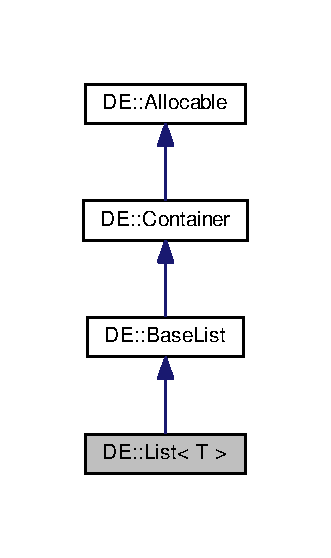
\includegraphics[width=159pt]{classDE_1_1List__inherit__graph}
\end{center}
\end{figure}


Collaboration diagram for DE\+:\+:List$<$ T $>$\+:\nopagebreak
\begin{figure}[H]
\begin{center}
\leavevmode
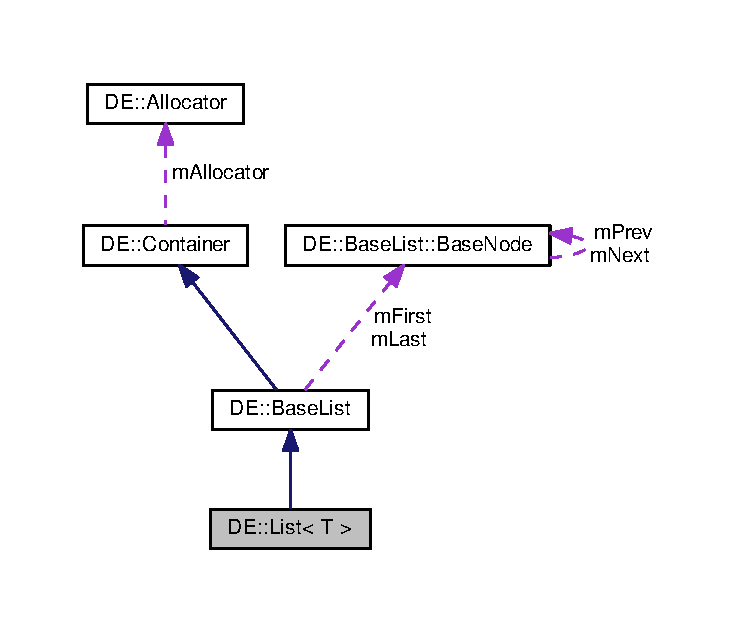
\includegraphics[width=350pt]{classDE_1_1List__coll__graph}
\end{center}
\end{figure}
\subsection*{Classes}
\begin{DoxyCompactItemize}
\item 
class \hyperlink{classDE_1_1List_1_1Iterator}{Iterator}
\end{DoxyCompactItemize}
\subsection*{Public Member Functions}
\begin{DoxyCompactItemize}
\item 
void {\bfseries init} (const \hyperlink{classDE_1_1List}{List} \&other)\hypertarget{classDE_1_1List_a939e1492cec40a32f386fbc3bfd3aad4}{}\label{classDE_1_1List_a939e1492cec40a32f386fbc3bfd3aad4}

\item 
void {\bfseries init} ()\hypertarget{classDE_1_1List_aaeced6c65cd99370cf78a19ba5f33d79}{}\label{classDE_1_1List_aaeced6c65cd99370cf78a19ba5f33d79}

\item 
\hyperlink{classDE_1_1List_1_1Iterator}{Iterator} {\bfseries get\+Iterator} () const \hypertarget{classDE_1_1List_ac3d3291c86f3305c42e335abdc59a742}{}\label{classDE_1_1List_ac3d3291c86f3305c42e335abdc59a742}

\item 
\hyperlink{classDE_1_1List_1_1Iterator}{Iterator} {\bfseries get\+Rev\+Iterator} () const \hypertarget{classDE_1_1List_abbef5a7352be5aa7dc1d83c1f4f97545}{}\label{classDE_1_1List_abbef5a7352be5aa7dc1d83c1f4f97545}

\item 
void {\bfseries push\+Front} (T element)\hypertarget{classDE_1_1List_a5b0ce6f5a23e9dbd8b0eb9ae33b98a90}{}\label{classDE_1_1List_a5b0ce6f5a23e9dbd8b0eb9ae33b98a90}

\item 
void {\bfseries push\+Back} (T element)\hypertarget{classDE_1_1List_a93687c23229ed4963ff46f356c890bb4}{}\label{classDE_1_1List_a93687c23229ed4963ff46f356c890bb4}

\item 
T {\bfseries pop\+Front} ()\hypertarget{classDE_1_1List_ae50e4be01d09c2358cc79ccc56957c8d}{}\label{classDE_1_1List_ae50e4be01d09c2358cc79ccc56957c8d}

\item 
T {\bfseries pop\+Back} ()\hypertarget{classDE_1_1List_a06c1593097f2543ca95b0d3bf5a6238c}{}\label{classDE_1_1List_a06c1593097f2543ca95b0d3bf5a6238c}

\item 
T {\bfseries get} (u32 index) const \hypertarget{classDE_1_1List_ad2ea5f64a6f88b5f4143e4c71b5cad90}{}\label{classDE_1_1List_ad2ea5f64a6f88b5f4143e4c71b5cad90}

\item 
void {\bfseries set} (u32 index, T element)\hypertarget{classDE_1_1List_a5e08633adfca77bec7f47117120ac5fd}{}\label{classDE_1_1List_a5e08633adfca77bec7f47117120ac5fd}

\item 
void {\bfseries swap} (u32 index1, u32 index2)\hypertarget{classDE_1_1List_a0d06f7ac8784ecf3f15f1469b3bb29bc}{}\label{classDE_1_1List_a0d06f7ac8784ecf3f15f1469b3bb29bc}

\item 
void {\bfseries remove} (u32 index)\hypertarget{classDE_1_1List_ab70462cf280a4459adb6c837fa20a494}{}\label{classDE_1_1List_ab70462cf280a4459adb6c837fa20a494}

\item 
void {\bfseries remove} (\hyperlink{classDE_1_1List_1_1Iterator}{Iterator} \&it)\hypertarget{classDE_1_1List_a91c378ed012e468dfdeb9796206fd70b}{}\label{classDE_1_1List_a91c378ed012e468dfdeb9796206fd70b}

\item 
void {\bfseries insert} (u32 index, T element)\hypertarget{classDE_1_1List_a24ce2d78bf3b79b4258a153e8b5701e6}{}\label{classDE_1_1List_a24ce2d78bf3b79b4258a153e8b5701e6}

\item 
void {\bfseries insert} (\hyperlink{classDE_1_1List_1_1Iterator}{Iterator} \&it, T element)\hypertarget{classDE_1_1List_a57232c3aa2cacad5458d79b04d20409b}{}\label{classDE_1_1List_a57232c3aa2cacad5458d79b04d20409b}

\item 
void {\bfseries sort} ()\hypertarget{classDE_1_1List_ac2fbbfb7910777429b31e43a003bb73c}{}\label{classDE_1_1List_ac2fbbfb7910777429b31e43a003bb73c}

\item 
void {\bfseries sort} (u8($\ast$comparator)(const T \&a, const T \&b))\hypertarget{classDE_1_1List_aca8907fcbb0da2c0f4edc43e6c83d40c}{}\label{classDE_1_1List_aca8907fcbb0da2c0f4edc43e6c83d40c}

\end{DoxyCompactItemize}
\subsection*{Additional Inherited Members}


The documentation for this class was generated from the following file\+:\begin{DoxyCompactItemize}
\item 
include/\+Containers/List.\+h\end{DoxyCompactItemize}

\hypertarget{classDE_1_1Matrix4}{}\section{DE\+:\+:Matrix4 Class Reference}
\label{classDE_1_1Matrix4}\index{D\+E\+::\+Matrix4@{D\+E\+::\+Matrix4}}
\subsection*{Public Member Functions}
\begin{DoxyCompactItemize}
\item 
void {\bfseries init} (const f32 n)\hypertarget{classDE_1_1Matrix4_a53c022b60ac40a372975f44b5e8839be}{}\label{classDE_1_1Matrix4_a53c022b60ac40a372975f44b5e8839be}

\item 
void {\bfseries init} (const \hyperlink{classDE_1_1Matrix4}{Matrix4} \&other)\hypertarget{classDE_1_1Matrix4_aa1c73280d1b281d32bcea3a9274212ec}{}\label{classDE_1_1Matrix4_aa1c73280d1b281d32bcea3a9274212ec}

\item 
void {\bfseries init} (\hyperlink{classDE_1_1Array}{Array}$<$ f32 $>$ \&data)\hypertarget{classDE_1_1Matrix4_a5098d65cbdfdbc3274746323b4215483}{}\label{classDE_1_1Matrix4_a5098d65cbdfdbc3274746323b4215483}

\item 
void {\bfseries init} (const \hyperlink{classDE_1_1Array}{Array}$<$ f32 $>$ \&row0, const \hyperlink{classDE_1_1Array}{Array}$<$ f32 $>$ \&row1, const \hyperlink{classDE_1_1Array}{Array}$<$ f32 $>$ \&row2, const \hyperlink{classDE_1_1Array}{Array}$<$ f32 $>$ \&row3)\hypertarget{classDE_1_1Matrix4_a41e8c30ef495235da98c5644aca35c20}{}\label{classDE_1_1Matrix4_a41e8c30ef495235da98c5644aca35c20}

\item 
void {\bfseries init} (const f32 $\ast$data)\hypertarget{classDE_1_1Matrix4_a534540f5569b22de93aff2c8f8929c1e}{}\label{classDE_1_1Matrix4_a534540f5569b22de93aff2c8f8929c1e}

\item 
void {\bfseries init} (const f32 $\ast$row0, const f32 $\ast$row1, const f32 $\ast$row2, const f32 $\ast$row3)\hypertarget{classDE_1_1Matrix4_abccd141001cd1fdbe62f01d1cb5d912d}{}\label{classDE_1_1Matrix4_abccd141001cd1fdbe62f01d1cb5d912d}

\item 
f32 $\ast$ {\bfseries get\+Data} ()\hypertarget{classDE_1_1Matrix4_af586b32a6b6e82b0ac4b896fcc41a014}{}\label{classDE_1_1Matrix4_af586b32a6b6e82b0ac4b896fcc41a014}

\item 
f32 {\bfseries get} (u8 row, u8 col)\hypertarget{classDE_1_1Matrix4_afc968e2fbe42762912618f766dc95518}{}\label{classDE_1_1Matrix4_afc968e2fbe42762912618f766dc95518}

\item 
void {\bfseries set} (u8 row, u8 col, f32 value)\hypertarget{classDE_1_1Matrix4_a38b0de6a91acebf6015cca263f34c036}{}\label{classDE_1_1Matrix4_a38b0de6a91acebf6015cca263f34c036}

\item 
void {\bfseries transpose} ()\hypertarget{classDE_1_1Matrix4_a6011b92a1c43331cdea2be7e2b51c45d}{}\label{classDE_1_1Matrix4_a6011b92a1c43331cdea2be7e2b51c45d}

\item 
void {\bfseries transpose} (\hyperlink{classDE_1_1Matrix4}{Matrix4} \&other)\hypertarget{classDE_1_1Matrix4_a4e1a75e4675a3dfd4bfab5d074321b7f}{}\label{classDE_1_1Matrix4_a4e1a75e4675a3dfd4bfab5d074321b7f}

\end{DoxyCompactItemize}


The documentation for this class was generated from the following files\+:\begin{DoxyCompactItemize}
\item 
include/\+Math/Matrix4.\+h\item 
source/\+Math/Matrix4.\+cpp\end{DoxyCompactItemize}

\hypertarget{classDE_1_1PoolAllocator}{}\section{DE\+:\+:Pool\+Allocator Class Reference}
\label{classDE_1_1PoolAllocator}\index{D\+E\+::\+Pool\+Allocator@{D\+E\+::\+Pool\+Allocator}}


Allocates memory using fixed-\/size blocks. The blocks can be freed.  




{\ttfamily \#include $<$Pool\+Allocator.\+h$>$}



Inheritance diagram for DE\+:\+:Pool\+Allocator\+:\nopagebreak
\begin{figure}[H]
\begin{center}
\leavevmode
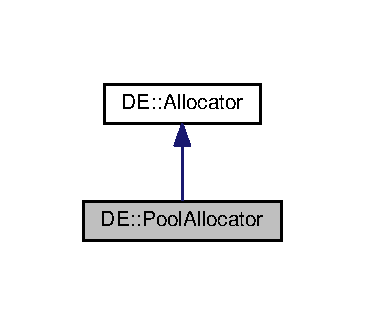
\includegraphics[width=175pt]{classDE_1_1PoolAllocator__inherit__graph}
\end{center}
\end{figure}


Collaboration diagram for DE\+:\+:Pool\+Allocator\+:\nopagebreak
\begin{figure}[H]
\begin{center}
\leavevmode
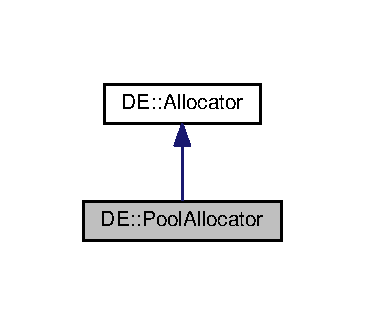
\includegraphics[width=175pt]{classDE_1_1PoolAllocator__coll__graph}
\end{center}
\end{figure}
\subsection*{Public Member Functions}
\begin{DoxyCompactItemize}
\item 
\hyperlink{classDE_1_1PoolAllocator_a337eec96091914fcb256b5aa0c88e057}{Pool\+Allocator} ()\hypertarget{classDE_1_1PoolAllocator_a337eec96091914fcb256b5aa0c88e057}{}\label{classDE_1_1PoolAllocator_a337eec96091914fcb256b5aa0c88e057}

\begin{DoxyCompactList}\small\item\em Default Constructor. \end{DoxyCompactList}\item 
virtual \hyperlink{classDE_1_1PoolAllocator_aa43fb65878a2843367907c0c7f87f601}{$\sim$\+Pool\+Allocator} ()\hypertarget{classDE_1_1PoolAllocator_aa43fb65878a2843367907c0c7f87f601}{}\label{classDE_1_1PoolAllocator_aa43fb65878a2843367907c0c7f87f601}

\begin{DoxyCompactList}\small\item\em Destructor. \end{DoxyCompactList}\item 
u32 \hyperlink{classDE_1_1PoolAllocator_abb72ae0c4f9cc376cdab99095bd02575}{get\+Free\+Blocks} ()
\item 
virtual void \hyperlink{classDE_1_1PoolAllocator_acd4f99952bffbe85c229d85ca60b164b}{init} (u32 block\+Size, u32 num\+Blocks, u32 alignment)
\begin{DoxyCompactList}\small\item\em Constructor. \end{DoxyCompactList}\item 
virtual void $\ast$ \hyperlink{classDE_1_1PoolAllocator_a55472e9fd8cbe6455706c781c1b1f2d9}{allocate} (u32 size)
\begin{DoxyCompactList}\small\item\em Allocates memory. \end{DoxyCompactList}\item 
virtual void $\ast$ \hyperlink{classDE_1_1PoolAllocator_a06a558e5d2b8a09b0a38ad8c6a4e100e}{allocate} (u32 size, u32 alignment)
\begin{DoxyCompactList}\small\item\em Allocates memory. \end{DoxyCompactList}\item 
void $\ast$ \hyperlink{classDE_1_1PoolAllocator_a1213fac1617eb643b185e03704e1d0f1}{allocate\+Block} ()
\begin{DoxyCompactList}\small\item\em Allocates a single block. \end{DoxyCompactList}\item 
virtual void \hyperlink{classDE_1_1PoolAllocator_ac8566e6920e0f34f70c2f76758fbb68a}{free} (const void $\ast$pointer)
\begin{DoxyCompactList}\small\item\em Frees memory. \end{DoxyCompactList}\item 
virtual void \hyperlink{classDE_1_1PoolAllocator_af20c44a50efd12448f87b268e308fc92}{free\+Aligned} (const void $\ast$pointer)
\begin{DoxyCompactList}\small\item\em Frees aligned memory. \end{DoxyCompactList}\item 
virtual void \hyperlink{classDE_1_1PoolAllocator_aa425fa59a6e3f2043e2cac2731cae393}{reset} ()\hypertarget{classDE_1_1PoolAllocator_aa425fa59a6e3f2043e2cac2731cae393}{}\label{classDE_1_1PoolAllocator_aa425fa59a6e3f2043e2cac2731cae393}

\begin{DoxyCompactList}\small\item\em Frees aligned memory. \end{DoxyCompactList}\end{DoxyCompactItemize}
\subsection*{Additional Inherited Members}


\subsection{Detailed Description}
Allocates memory using fixed-\/size blocks. The blocks can be freed. 

\subsection{Member Function Documentation}
\index{D\+E\+::\+Pool\+Allocator@{D\+E\+::\+Pool\+Allocator}!allocate@{allocate}}
\index{allocate@{allocate}!D\+E\+::\+Pool\+Allocator@{D\+E\+::\+Pool\+Allocator}}
\subsubsection[{\texorpdfstring{allocate(u32 size)}{allocate(u32 size)}}]{\setlength{\rightskip}{0pt plus 5cm}void $\ast$ D\+E\+::\+Pool\+Allocator\+::allocate (
\begin{DoxyParamCaption}
\item[{u32}]{size}
\end{DoxyParamCaption}
)\hspace{0.3cm}{\ttfamily [virtual]}}\hypertarget{classDE_1_1PoolAllocator_a55472e9fd8cbe6455706c781c1b1f2d9}{}\label{classDE_1_1PoolAllocator_a55472e9fd8cbe6455706c781c1b1f2d9}


Allocates memory. 


\begin{DoxyParams}{Parameters}
{\em size} & Amount of memory you want to allocate. \\
\hline
\end{DoxyParams}
\begin{DoxyReturn}{Returns}
Pointer to memory chunk. 
\end{DoxyReturn}


Implements \hyperlink{classDE_1_1Allocator_a25c66f6c09ca69ef083219fc7c2b0392}{D\+E\+::\+Allocator}.

\index{D\+E\+::\+Pool\+Allocator@{D\+E\+::\+Pool\+Allocator}!allocate@{allocate}}
\index{allocate@{allocate}!D\+E\+::\+Pool\+Allocator@{D\+E\+::\+Pool\+Allocator}}
\subsubsection[{\texorpdfstring{allocate(u32 size, u32 alignment)}{allocate(u32 size, u32 alignment)}}]{\setlength{\rightskip}{0pt plus 5cm}void $\ast$ D\+E\+::\+Pool\+Allocator\+::allocate (
\begin{DoxyParamCaption}
\item[{u32}]{size, }
\item[{u32}]{alignment}
\end{DoxyParamCaption}
)\hspace{0.3cm}{\ttfamily [virtual]}}\hypertarget{classDE_1_1PoolAllocator_a06a558e5d2b8a09b0a38ad8c6a4e100e}{}\label{classDE_1_1PoolAllocator_a06a558e5d2b8a09b0a38ad8c6a4e100e}


Allocates memory. 


\begin{DoxyParams}{Parameters}
{\em size} & Amount of memory you want to allocate. \\
\hline
{\em alignment} & Bytes alignment. \\
\hline
\end{DoxyParams}
\begin{DoxyReturn}{Returns}
Pointer to memory chunk. 
\end{DoxyReturn}


Implements \hyperlink{classDE_1_1Allocator_ae8e197bc4bab60a9321b8c25596e927d}{D\+E\+::\+Allocator}.

\index{D\+E\+::\+Pool\+Allocator@{D\+E\+::\+Pool\+Allocator}!allocate\+Block@{allocate\+Block}}
\index{allocate\+Block@{allocate\+Block}!D\+E\+::\+Pool\+Allocator@{D\+E\+::\+Pool\+Allocator}}
\subsubsection[{\texorpdfstring{allocate\+Block()}{allocateBlock()}}]{\setlength{\rightskip}{0pt plus 5cm}void $\ast$ D\+E\+::\+Pool\+Allocator\+::allocate\+Block (
\begin{DoxyParamCaption}
{}
\end{DoxyParamCaption}
)}\hypertarget{classDE_1_1PoolAllocator_a1213fac1617eb643b185e03704e1d0f1}{}\label{classDE_1_1PoolAllocator_a1213fac1617eb643b185e03704e1d0f1}


Allocates a single block. 

\begin{DoxyReturn}{Returns}
Pointer to the new block. 
\end{DoxyReturn}
\index{D\+E\+::\+Pool\+Allocator@{D\+E\+::\+Pool\+Allocator}!free@{free}}
\index{free@{free}!D\+E\+::\+Pool\+Allocator@{D\+E\+::\+Pool\+Allocator}}
\subsubsection[{\texorpdfstring{free(const void $\ast$pointer)}{free(const void *pointer)}}]{\setlength{\rightskip}{0pt plus 5cm}void D\+E\+::\+Pool\+Allocator\+::free (
\begin{DoxyParamCaption}
\item[{const void $\ast$}]{pointer}
\end{DoxyParamCaption}
)\hspace{0.3cm}{\ttfamily [virtual]}}\hypertarget{classDE_1_1PoolAllocator_ac8566e6920e0f34f70c2f76758fbb68a}{}\label{classDE_1_1PoolAllocator_ac8566e6920e0f34f70c2f76758fbb68a}


Frees memory. 


\begin{DoxyParams}{Parameters}
{\em pointer} & Pointer to memory. \\
\hline
\end{DoxyParams}


Implements \hyperlink{classDE_1_1Allocator_a9a01f5da5adafc6d5cee9b3e3e9859c4}{D\+E\+::\+Allocator}.

\index{D\+E\+::\+Pool\+Allocator@{D\+E\+::\+Pool\+Allocator}!free\+Aligned@{free\+Aligned}}
\index{free\+Aligned@{free\+Aligned}!D\+E\+::\+Pool\+Allocator@{D\+E\+::\+Pool\+Allocator}}
\subsubsection[{\texorpdfstring{free\+Aligned(const void $\ast$pointer)}{freeAligned(const void *pointer)}}]{\setlength{\rightskip}{0pt plus 5cm}void D\+E\+::\+Pool\+Allocator\+::free\+Aligned (
\begin{DoxyParamCaption}
\item[{const void $\ast$}]{pointer}
\end{DoxyParamCaption}
)\hspace{0.3cm}{\ttfamily [virtual]}}\hypertarget{classDE_1_1PoolAllocator_af20c44a50efd12448f87b268e308fc92}{}\label{classDE_1_1PoolAllocator_af20c44a50efd12448f87b268e308fc92}


Frees aligned memory. 


\begin{DoxyParams}{Parameters}
{\em pointer} & Pointer to aligned memory. \\
\hline
\end{DoxyParams}


Implements \hyperlink{classDE_1_1Allocator_a765f3ff9d6ff095bdfe4674652542a3d}{D\+E\+::\+Allocator}.

\index{D\+E\+::\+Pool\+Allocator@{D\+E\+::\+Pool\+Allocator}!get\+Free\+Blocks@{get\+Free\+Blocks}}
\index{get\+Free\+Blocks@{get\+Free\+Blocks}!D\+E\+::\+Pool\+Allocator@{D\+E\+::\+Pool\+Allocator}}
\subsubsection[{\texorpdfstring{get\+Free\+Blocks()}{getFreeBlocks()}}]{\setlength{\rightskip}{0pt plus 5cm}u32 D\+E\+::\+Pool\+Allocator\+::get\+Free\+Blocks (
\begin{DoxyParamCaption}
{}
\end{DoxyParamCaption}
)}\hypertarget{classDE_1_1PoolAllocator_abb72ae0c4f9cc376cdab99095bd02575}{}\label{classDE_1_1PoolAllocator_abb72ae0c4f9cc376cdab99095bd02575}
\begin{DoxyReturn}{Returns}
The count of free blocks. 
\end{DoxyReturn}
\index{D\+E\+::\+Pool\+Allocator@{D\+E\+::\+Pool\+Allocator}!init@{init}}
\index{init@{init}!D\+E\+::\+Pool\+Allocator@{D\+E\+::\+Pool\+Allocator}}
\subsubsection[{\texorpdfstring{init(u32 block\+Size, u32 num\+Blocks, u32 alignment)}{init(u32 blockSize, u32 numBlocks, u32 alignment)}}]{\setlength{\rightskip}{0pt plus 5cm}void D\+E\+::\+Pool\+Allocator\+::init (
\begin{DoxyParamCaption}
\item[{u32}]{block\+Size, }
\item[{u32}]{num\+Blocks, }
\item[{u32}]{alignment}
\end{DoxyParamCaption}
)\hspace{0.3cm}{\ttfamily [virtual]}}\hypertarget{classDE_1_1PoolAllocator_acd4f99952bffbe85c229d85ca60b164b}{}\label{classDE_1_1PoolAllocator_acd4f99952bffbe85c229d85ca60b164b}


Constructor. 


\begin{DoxyParams}{Parameters}
{\em block\+Size} & Size of a single block. \\
\hline
{\em num\+Blocks} & Number of blocks. \\
\hline
{\em alignment} & Bytes alignment. \\
\hline
\end{DoxyParams}


The documentation for this class was generated from the following files\+:\begin{DoxyCompactItemize}
\item 
include/\+Memory/Pool\+Allocator.\+h\item 
source/\+Memory/Pool\+Allocator.\+cpp\end{DoxyCompactItemize}

\hypertarget{classDE_1_1Quaternion}{}\section{DE\+:\+:Quaternion Class Reference}
\label{classDE_1_1Quaternion}\index{D\+E\+::\+Quaternion@{D\+E\+::\+Quaternion}}


Collaboration diagram for DE\+:\+:Quaternion\+:
\nopagebreak
\begin{figure}[H]
\begin{center}
\leavevmode
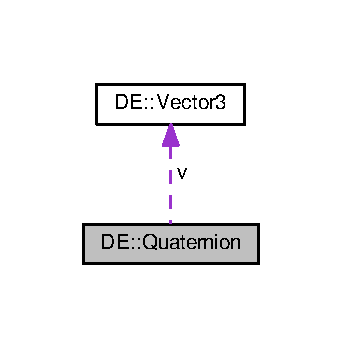
\includegraphics[width=164pt]{classDE_1_1Quaternion__coll__graph}
\end{center}
\end{figure}
\subsection*{Public Member Functions}
\begin{DoxyCompactItemize}
\item 
{\bfseries Quaternion} (f32 x, f32 y, f32 z, f32 w)\hypertarget{classDE_1_1Quaternion_a46fdded1aa5d3e869d3d72e07586890c}{}\label{classDE_1_1Quaternion_a46fdded1aa5d3e869d3d72e07586890c}

\item 
{\bfseries Quaternion} (const \hyperlink{classDE_1_1Vector3}{Vector3} \&v, f32 w)\hypertarget{classDE_1_1Quaternion_a8e2c0a32e74e099eaf8e7f468513ccad}{}\label{classDE_1_1Quaternion_a8e2c0a32e74e099eaf8e7f468513ccad}

\item 
{\bfseries Quaternion} (f32 theta\+\_\+x, f32 theta\+\_\+y, f32 theta\+\_\+z)\hypertarget{classDE_1_1Quaternion_a16ca7374edb7f228a9f2d641da614b4c}{}\label{classDE_1_1Quaternion_a16ca7374edb7f228a9f2d641da614b4c}

\item 
{\bfseries Quaternion} (const \hyperlink{classDE_1_1Vector3}{Vector3} \&v)\hypertarget{classDE_1_1Quaternion_a71d7271ec4982e0ef4b35cde0ef538ce}{}\label{classDE_1_1Quaternion_a71d7271ec4982e0ef4b35cde0ef538ce}

\item 
{\bfseries Quaternion} (const \hyperlink{classDE_1_1Quaternion}{Quaternion} \&other)\hypertarget{classDE_1_1Quaternion_a859e5db839c584aeb7b28a8b799c2041}{}\label{classDE_1_1Quaternion_a859e5db839c584aeb7b28a8b799c2041}

\item 
\hyperlink{classDE_1_1Quaternion}{Quaternion} \& {\bfseries set} (f32 x, f32 y, f32 z, f32 w)\hypertarget{classDE_1_1Quaternion_ac64303fb77f95fa307aa6fffb9536aec}{}\label{classDE_1_1Quaternion_ac64303fb77f95fa307aa6fffb9536aec}

\item 
\hyperlink{classDE_1_1Quaternion}{Quaternion} \& {\bfseries set} (const \hyperlink{classDE_1_1Vector3}{Vector3} \&v, f32 w)\hypertarget{classDE_1_1Quaternion_a43d98814114d82aedabf4dd27fe13184}{}\label{classDE_1_1Quaternion_a43d98814114d82aedabf4dd27fe13184}

\item 
\hyperlink{classDE_1_1Quaternion}{Quaternion} \& {\bfseries set} (const \hyperlink{classDE_1_1Quaternion}{Quaternion} \&rhs)\hypertarget{classDE_1_1Quaternion_ae68c59723bfbd7be5869453716a804c4}{}\label{classDE_1_1Quaternion_ae68c59723bfbd7be5869453716a804c4}

\item 
\hyperlink{classDE_1_1Quaternion}{Quaternion} \& {\bfseries add} (const \hyperlink{classDE_1_1Quaternion}{Quaternion} \&rhs)\hypertarget{classDE_1_1Quaternion_ad7d74159c0b16aca62990fcab61613f3}{}\label{classDE_1_1Quaternion_ad7d74159c0b16aca62990fcab61613f3}

\item 
\hyperlink{classDE_1_1Quaternion}{Quaternion} \& {\bfseries sub} (const \hyperlink{classDE_1_1Quaternion}{Quaternion} \&rhs)\hypertarget{classDE_1_1Quaternion_ab5661a337143dd2d31dfbe84958f02d2}{}\label{classDE_1_1Quaternion_ab5661a337143dd2d31dfbe84958f02d2}

\item 
\hyperlink{classDE_1_1Quaternion}{Quaternion} \& {\bfseries mul} (const \hyperlink{classDE_1_1Quaternion}{Quaternion} \&rhs)\hypertarget{classDE_1_1Quaternion_a394687030fec375b1d52fc5e86f80362}{}\label{classDE_1_1Quaternion_a394687030fec375b1d52fc5e86f80362}

\item 
\hyperlink{classDE_1_1Quaternion}{Quaternion} \& {\bfseries div} (const \hyperlink{classDE_1_1Quaternion}{Quaternion} \&rhs)\hypertarget{classDE_1_1Quaternion_a9c88cf74bec9e0284b951f65647d0782}{}\label{classDE_1_1Quaternion_a9c88cf74bec9e0284b951f65647d0782}

\item 
\hyperlink{classDE_1_1Quaternion}{Quaternion} \& {\bfseries add} (const f32 rhs)\hypertarget{classDE_1_1Quaternion_ae4858fc96078dcfe4f2dff0f8a4ac698}{}\label{classDE_1_1Quaternion_ae4858fc96078dcfe4f2dff0f8a4ac698}

\item 
\hyperlink{classDE_1_1Quaternion}{Quaternion} \& {\bfseries sub} (const f32 rhs)\hypertarget{classDE_1_1Quaternion_abe307909b9803fd2757e34e20a49f41e}{}\label{classDE_1_1Quaternion_abe307909b9803fd2757e34e20a49f41e}

\item 
\hyperlink{classDE_1_1Quaternion}{Quaternion} \& {\bfseries mul} (const f32 rhs)\hypertarget{classDE_1_1Quaternion_a684c887ab5a3c05d8b7319dddac20bd1}{}\label{classDE_1_1Quaternion_a684c887ab5a3c05d8b7319dddac20bd1}

\item 
\hyperlink{classDE_1_1Quaternion}{Quaternion} \& {\bfseries div} (const f32 rhs)\hypertarget{classDE_1_1Quaternion_a6db27bf99aeb7b12c4d800f8768eb387}{}\label{classDE_1_1Quaternion_a6db27bf99aeb7b12c4d800f8768eb387}

\item 
f32 {\bfseries len} () const \hypertarget{classDE_1_1Quaternion_ab8f9a95f1b2c532a8aece1c6cd04a76a}{}\label{classDE_1_1Quaternion_ab8f9a95f1b2c532a8aece1c6cd04a76a}

\item 
f32 {\bfseries sqrlen} () const \hypertarget{classDE_1_1Quaternion_a3ae52b98d4d41cbe4bb596d864951137}{}\label{classDE_1_1Quaternion_a3ae52b98d4d41cbe4bb596d864951137}

\item 
f32 {\bfseries dot} (const \hyperlink{classDE_1_1Quaternion}{Quaternion} \&q) const \hypertarget{classDE_1_1Quaternion_a7daa47280a1fe53ea68c674c46066bc5}{}\label{classDE_1_1Quaternion_a7daa47280a1fe53ea68c674c46066bc5}

\item 
\hyperlink{classDE_1_1Quaternion}{Quaternion} \& {\bfseries nor} ()\hypertarget{classDE_1_1Quaternion_aef4f30484499792f39b86139bb2e4773}{}\label{classDE_1_1Quaternion_aef4f30484499792f39b86139bb2e4773}

\item 
bool {\bfseries eq} (const \hyperlink{classDE_1_1Quaternion}{Quaternion} \&q, f32 e) const \hypertarget{classDE_1_1Quaternion_adce228837e893238f875a09e92a1ab8b}{}\label{classDE_1_1Quaternion_adce228837e893238f875a09e92a1ab8b}

\item 
bool {\bfseries eq} (const \hyperlink{classDE_1_1Quaternion}{Quaternion} \&q) const \hypertarget{classDE_1_1Quaternion_ae48d93a80a27d1e8e3e61f77cac26220}{}\label{classDE_1_1Quaternion_ae48d93a80a27d1e8e3e61f77cac26220}

\item 
\hyperlink{classDE_1_1Quaternion}{Quaternion} \& {\bfseries conj} ()\hypertarget{classDE_1_1Quaternion_a34f7d52202de842302965e579845110b}{}\label{classDE_1_1Quaternion_a34f7d52202de842302965e579845110b}

\item 
\hyperlink{classDE_1_1Quaternion}{Quaternion} \& {\bfseries inv} ()\hypertarget{classDE_1_1Quaternion_a15439b8377007d11707aec0e225743b4}{}\label{classDE_1_1Quaternion_a15439b8377007d11707aec0e225743b4}

\item 
\hyperlink{classDE_1_1Quaternion}{Quaternion} \& {\bfseries lerp} (const \hyperlink{classDE_1_1Quaternion}{Quaternion} \&target, f32 t)\hypertarget{classDE_1_1Quaternion_a76110c16875cb15ac7a6c8feb79ce0cb}{}\label{classDE_1_1Quaternion_a76110c16875cb15ac7a6c8feb79ce0cb}

\item 
\hyperlink{classDE_1_1Quaternion}{Quaternion} \& {\bfseries nlerp} (const \hyperlink{classDE_1_1Quaternion}{Quaternion} \&target, f32 t)\hypertarget{classDE_1_1Quaternion_a8f97c9312327a9ff2069e391349da34e}{}\label{classDE_1_1Quaternion_a8f97c9312327a9ff2069e391349da34e}

\item 
\hyperlink{classDE_1_1Quaternion}{Quaternion} \& {\bfseries slerp} (const \hyperlink{classDE_1_1Quaternion}{Quaternion} \&target, f32 t)\hypertarget{classDE_1_1Quaternion_a3fcaa1da829ddf6d0903107d5c0f8073}{}\label{classDE_1_1Quaternion_a3fcaa1da829ddf6d0903107d5c0f8073}

\item 
\hyperlink{classDE_1_1Quaternion}{Quaternion} \& {\bfseries squad} ()\hypertarget{classDE_1_1Quaternion_aed1e82935603e88c25e9e7f9e3a64c9d}{}\label{classDE_1_1Quaternion_aed1e82935603e88c25e9e7f9e3a64c9d}

\item 
\hyperlink{classDE_1_1Vector3}{Vector3} {\bfseries to\+Euler} () const \hypertarget{classDE_1_1Quaternion_a2a160c16c4af3a3c7651d5192a5b179f}{}\label{classDE_1_1Quaternion_a2a160c16c4af3a3c7651d5192a5b179f}

\item 
f32 {\bfseries angle} (const \hyperlink{classDE_1_1Quaternion}{Quaternion} \&q) const \hypertarget{classDE_1_1Quaternion_a7e353f105456279d39ef2d72e26cad1e}{}\label{classDE_1_1Quaternion_a7e353f105456279d39ef2d72e26cad1e}

\item 
\hyperlink{classDE_1_1Quaternion}{Quaternion} \& {\bfseries operator=} (const \hyperlink{classDE_1_1Quaternion}{Quaternion} \&rhs)\hypertarget{classDE_1_1Quaternion_ad2da76b8c7c4e4680459c0196f7d5acc}{}\label{classDE_1_1Quaternion_ad2da76b8c7c4e4680459c0196f7d5acc}

\item 
\hyperlink{classDE_1_1Quaternion}{Quaternion} \& {\bfseries operator+=} (const \hyperlink{classDE_1_1Quaternion}{Quaternion} \&rhs)\hypertarget{classDE_1_1Quaternion_a0f42351a48a8f17b0b4389f7be8ca2ee}{}\label{classDE_1_1Quaternion_a0f42351a48a8f17b0b4389f7be8ca2ee}

\item 
\hyperlink{classDE_1_1Quaternion}{Quaternion} \& {\bfseries operator-\/=} (const \hyperlink{classDE_1_1Quaternion}{Quaternion} \&rhs)\hypertarget{classDE_1_1Quaternion_a980925ab488d5af6a76691c9d06a5f15}{}\label{classDE_1_1Quaternion_a980925ab488d5af6a76691c9d06a5f15}

\item 
\hyperlink{classDE_1_1Quaternion}{Quaternion} \& {\bfseries operator$\ast$=} (const \hyperlink{classDE_1_1Quaternion}{Quaternion} \&rhs)\hypertarget{classDE_1_1Quaternion_aa417617c70e6e537c2d7de1c51461388}{}\label{classDE_1_1Quaternion_aa417617c70e6e537c2d7de1c51461388}

\item 
\hyperlink{classDE_1_1Quaternion}{Quaternion} \& {\bfseries operator/=} (const \hyperlink{classDE_1_1Quaternion}{Quaternion} \&rhs)\hypertarget{classDE_1_1Quaternion_a6c77fb19ad3da7d7a8443de9bd3440b4}{}\label{classDE_1_1Quaternion_a6c77fb19ad3da7d7a8443de9bd3440b4}

\item 
\hyperlink{classDE_1_1Quaternion}{Quaternion} \& {\bfseries operator+=} (const f32 rhs)\hypertarget{classDE_1_1Quaternion_a9adc1894db7e9c6cd1434c42ca9ad8bd}{}\label{classDE_1_1Quaternion_a9adc1894db7e9c6cd1434c42ca9ad8bd}

\item 
\hyperlink{classDE_1_1Quaternion}{Quaternion} \& {\bfseries operator-\/=} (const f32 rhs)\hypertarget{classDE_1_1Quaternion_ac84af02c048b5dc3d57d579b7b686df9}{}\label{classDE_1_1Quaternion_ac84af02c048b5dc3d57d579b7b686df9}

\item 
\hyperlink{classDE_1_1Quaternion}{Quaternion} \& {\bfseries operator$\ast$=} (const f32 rhs)\hypertarget{classDE_1_1Quaternion_a77c7449a159ea34a7d19f49d560f89d3}{}\label{classDE_1_1Quaternion_a77c7449a159ea34a7d19f49d560f89d3}

\item 
\hyperlink{classDE_1_1Quaternion}{Quaternion} \& {\bfseries operator/=} (const f32 rhs)\hypertarget{classDE_1_1Quaternion_ac2ee7e70fea139eeae6b16bd331f60b7}{}\label{classDE_1_1Quaternion_ac2ee7e70fea139eeae6b16bd331f60b7}

\item 
bool {\bfseries operator==} (const \hyperlink{classDE_1_1Quaternion}{Quaternion} \&rhs) const \hypertarget{classDE_1_1Quaternion_a53df6aa56fdb298bd9445e422b54fbf6}{}\label{classDE_1_1Quaternion_a53df6aa56fdb298bd9445e422b54fbf6}

\item 
bool {\bfseries operator!=} (const \hyperlink{classDE_1_1Quaternion}{Quaternion} \&rhs) const \hypertarget{classDE_1_1Quaternion_ad0da0623153e0ea2fbd54dbe7d44632d}{}\label{classDE_1_1Quaternion_ad0da0623153e0ea2fbd54dbe7d44632d}

\item 
\hyperlink{classDE_1_1Quaternion}{Quaternion} {\bfseries operator+} (const \hyperlink{classDE_1_1Quaternion}{Quaternion} \&rhs) const \hypertarget{classDE_1_1Quaternion_ae16394793eafa20de7b7ab46de3fe2e7}{}\label{classDE_1_1Quaternion_ae16394793eafa20de7b7ab46de3fe2e7}

\item 
\hyperlink{classDE_1_1Quaternion}{Quaternion} {\bfseries operator-\/} (const \hyperlink{classDE_1_1Quaternion}{Quaternion} \&rhs) const \hypertarget{classDE_1_1Quaternion_ae131ef219cd4ee80c5bf65920f33a1cc}{}\label{classDE_1_1Quaternion_ae131ef219cd4ee80c5bf65920f33a1cc}

\item 
\hyperlink{classDE_1_1Quaternion}{Quaternion} {\bfseries operator$\ast$} (const \hyperlink{classDE_1_1Quaternion}{Quaternion} \&rhs) const \hypertarget{classDE_1_1Quaternion_a1daa7c9b461cee784f5801fe3e0dabb0}{}\label{classDE_1_1Quaternion_a1daa7c9b461cee784f5801fe3e0dabb0}

\item 
\hyperlink{classDE_1_1Quaternion}{Quaternion} {\bfseries operator/} (const \hyperlink{classDE_1_1Quaternion}{Quaternion} \&rhs) const \hypertarget{classDE_1_1Quaternion_a7ad349509dff622a707a94e1336b7276}{}\label{classDE_1_1Quaternion_a7ad349509dff622a707a94e1336b7276}

\item 
\hyperlink{classDE_1_1Quaternion}{Quaternion} {\bfseries operator+} (const f32 rhs) const \hypertarget{classDE_1_1Quaternion_aa24ad6dd4e596535b4929cbc14a675b3}{}\label{classDE_1_1Quaternion_aa24ad6dd4e596535b4929cbc14a675b3}

\item 
\hyperlink{classDE_1_1Quaternion}{Quaternion} {\bfseries operator-\/} (const f32 rhs) const \hypertarget{classDE_1_1Quaternion_a3c9d672c1e7d5ba7dc494af75efe7f1c}{}\label{classDE_1_1Quaternion_a3c9d672c1e7d5ba7dc494af75efe7f1c}

\item 
\hyperlink{classDE_1_1Quaternion}{Quaternion} {\bfseries operator$\ast$} (const f32 rhs) const \hypertarget{classDE_1_1Quaternion_ac3bf880b24c8b02bb4a296494c3b2085}{}\label{classDE_1_1Quaternion_ac3bf880b24c8b02bb4a296494c3b2085}

\item 
\hyperlink{classDE_1_1Quaternion}{Quaternion} {\bfseries operator/} (const f32 rhs) const \hypertarget{classDE_1_1Quaternion_afbd3dc214dec6f05dbbbaf9573066e3f}{}\label{classDE_1_1Quaternion_afbd3dc214dec6f05dbbbaf9573066e3f}

\item 
f32 \& {\bfseries operator\mbox{[}$\,$\mbox{]}} (const size\+\_\+t i)\hypertarget{classDE_1_1Quaternion_aa1326ce5206f5a112704bf42002ddf56}{}\label{classDE_1_1Quaternion_aa1326ce5206f5a112704bf42002ddf56}

\item 
f32 {\bfseries operator\mbox{[}$\,$\mbox{]}} (const size\+\_\+t i) const \hypertarget{classDE_1_1Quaternion_abe6b9626b48bb341a56e0e5187d09dc6}{}\label{classDE_1_1Quaternion_abe6b9626b48bb341a56e0e5187d09dc6}

\end{DoxyCompactItemize}
\subsection*{Public Attributes}
\begin{DoxyCompactItemize}
\item 
f32 {\bfseries w}\hypertarget{classDE_1_1Quaternion_a95b5773a30c217a32176518000311287}{}\label{classDE_1_1Quaternion_a95b5773a30c217a32176518000311287}

\item 
\hyperlink{classDE_1_1Vector3}{Vector3} {\bfseries v}\hypertarget{classDE_1_1Quaternion_a23bc86f9e49c7df4bb98cf0bfd9762f7}{}\label{classDE_1_1Quaternion_a23bc86f9e49c7df4bb98cf0bfd9762f7}

\end{DoxyCompactItemize}
\subsection*{Friends}
\begin{DoxyCompactItemize}
\item 
std\+::ostream \& {\bfseries operator$<$$<$} (std\+::ostream \&out, const \hyperlink{classDE_1_1Quaternion}{Quaternion} \&q)\hypertarget{classDE_1_1Quaternion_a9d6837ef4f759aa5ecd417adcea2e908}{}\label{classDE_1_1Quaternion_a9d6837ef4f759aa5ecd417adcea2e908}

\end{DoxyCompactItemize}


The documentation for this class was generated from the following files\+:\begin{DoxyCompactItemize}
\item 
include/\+Math/Quaternion.\+h\item 
source/\+Math/Quaternion.\+cpp\end{DoxyCompactItemize}

\hypertarget{classDE_1_1StackAllocator}{}\section{DE\+:\+:Stack\+Allocator Class Reference}
\label{classDE_1_1StackAllocator}\index{D\+E\+::\+Stack\+Allocator@{D\+E\+::\+Stack\+Allocator}}


Allocates memory in F\+I\+FO strategy.  




{\ttfamily \#include $<$Stack\+Allocator.\+h$>$}



Inheritance diagram for DE\+:\+:Stack\+Allocator\+:
\nopagebreak
\begin{figure}[H]
\begin{center}
\leavevmode
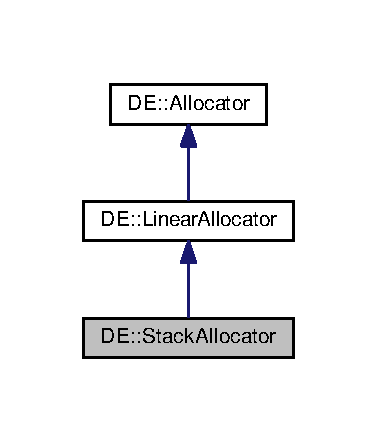
\includegraphics[width=181pt]{classDE_1_1StackAllocator__inherit__graph}
\end{center}
\end{figure}


Collaboration diagram for DE\+:\+:Stack\+Allocator\+:
\nopagebreak
\begin{figure}[H]
\begin{center}
\leavevmode
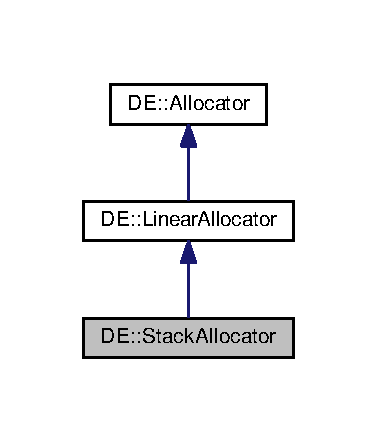
\includegraphics[width=181pt]{classDE_1_1StackAllocator__coll__graph}
\end{center}
\end{figure}
\subsection*{Public Member Functions}
\begin{DoxyCompactItemize}
\item 
\hyperlink{classDE_1_1StackAllocator_a71869927ff38ef330d4146bc1c2608c7}{Stack\+Allocator} ()\hypertarget{classDE_1_1StackAllocator_a71869927ff38ef330d4146bc1c2608c7}{}\label{classDE_1_1StackAllocator_a71869927ff38ef330d4146bc1c2608c7}

\begin{DoxyCompactList}\small\item\em Default Constructor. \end{DoxyCompactList}\item 
virtual \hyperlink{classDE_1_1StackAllocator_a6e680f39f10b1f07ae7d3bd485138abc}{$\sim$\+Stack\+Allocator} ()\hypertarget{classDE_1_1StackAllocator_a6e680f39f10b1f07ae7d3bd485138abc}{}\label{classDE_1_1StackAllocator_a6e680f39f10b1f07ae7d3bd485138abc}

\begin{DoxyCompactList}\small\item\em Destructor. \end{DoxyCompactList}\item 
void $\ast$ \hyperlink{classDE_1_1StackAllocator_a338da3513a5d49abb8ac7191b5201c37}{get\+Top} ()
\item 
virtual void \hyperlink{classDE_1_1StackAllocator_a529ba39bd01e84cdb140db3343a7bf50}{init} (u32 size)
\begin{DoxyCompactList}\small\item\em Constructor. \end{DoxyCompactList}\item 
virtual void $\ast$ \hyperlink{classDE_1_1StackAllocator_a4b360ed983169d4063d0b85ac83ec156}{allocate} (u32 size)
\begin{DoxyCompactList}\small\item\em Allocates memory. \end{DoxyCompactList}\item 
virtual void $\ast$ \hyperlink{classDE_1_1StackAllocator_afa3e49ff8c47278c25e8ffcfa7897a80}{allocate} (u32 size, u32 alignment)
\begin{DoxyCompactList}\small\item\em Allocates memory. \end{DoxyCompactList}\item 
virtual void \hyperlink{classDE_1_1StackAllocator_ae1c77f32df6421293da96dc322f33c98}{free} (const void $\ast$pointer)
\begin{DoxyCompactList}\small\item\em Frees memory. \end{DoxyCompactList}\item 
virtual void \hyperlink{classDE_1_1StackAllocator_aac3d433b63805fbd046a3ce70d6d6305}{free\+Aligned} (const void $\ast$pointer)
\begin{DoxyCompactList}\small\item\em Frees aligned memory. \end{DoxyCompactList}\item 
void \hyperlink{classDE_1_1StackAllocator_a30cba40c244648427e741766d2f26ab7}{free} ()\hypertarget{classDE_1_1StackAllocator_a30cba40c244648427e741766d2f26ab7}{}\label{classDE_1_1StackAllocator_a30cba40c244648427e741766d2f26ab7}

\begin{DoxyCompactList}\small\item\em Free the top of the stack. \end{DoxyCompactList}\item 
void \hyperlink{classDE_1_1StackAllocator_ab85d29fe77b49d3b809ddb89ea2e0ed6}{free\+Aligned} ()\hypertarget{classDE_1_1StackAllocator_ab85d29fe77b49d3b809ddb89ea2e0ed6}{}\label{classDE_1_1StackAllocator_ab85d29fe77b49d3b809ddb89ea2e0ed6}

\begin{DoxyCompactList}\small\item\em Free the (aligned) top of the stack. \end{DoxyCompactList}\item 
virtual void \hyperlink{classDE_1_1StackAllocator_a65370aba2f33a0f04f9e49fec85fb4c8}{reset} ()\hypertarget{classDE_1_1StackAllocator_a65370aba2f33a0f04f9e49fec85fb4c8}{}\label{classDE_1_1StackAllocator_a65370aba2f33a0f04f9e49fec85fb4c8}

\begin{DoxyCompactList}\small\item\em Frees aligned memory. \end{DoxyCompactList}\end{DoxyCompactItemize}
\subsection*{Additional Inherited Members}


\subsection{Detailed Description}
Allocates memory in F\+I\+FO strategy. 

\subsection{Member Function Documentation}
\index{D\+E\+::\+Stack\+Allocator@{D\+E\+::\+Stack\+Allocator}!allocate@{allocate}}
\index{allocate@{allocate}!D\+E\+::\+Stack\+Allocator@{D\+E\+::\+Stack\+Allocator}}
\subsubsection[{\texorpdfstring{allocate(u32 size)}{allocate(u32 size)}}]{\setlength{\rightskip}{0pt plus 5cm}void $\ast$ D\+E\+::\+Stack\+Allocator\+::allocate (
\begin{DoxyParamCaption}
\item[{u32}]{size}
\end{DoxyParamCaption}
)\hspace{0.3cm}{\ttfamily [virtual]}}\hypertarget{classDE_1_1StackAllocator_a4b360ed983169d4063d0b85ac83ec156}{}\label{classDE_1_1StackAllocator_a4b360ed983169d4063d0b85ac83ec156}


Allocates memory. 


\begin{DoxyParams}{Parameters}
{\em size} & Amount of memory you want to allocate. \\
\hline
\end{DoxyParams}
\begin{DoxyReturn}{Returns}
Pointer to memory chunk. 
\end{DoxyReturn}


Reimplemented from \hyperlink{classDE_1_1LinearAllocator_a4758d08eb92d0a78a614d40822180ae4}{D\+E\+::\+Linear\+Allocator}.

\index{D\+E\+::\+Stack\+Allocator@{D\+E\+::\+Stack\+Allocator}!allocate@{allocate}}
\index{allocate@{allocate}!D\+E\+::\+Stack\+Allocator@{D\+E\+::\+Stack\+Allocator}}
\subsubsection[{\texorpdfstring{allocate(u32 size, u32 alignment)}{allocate(u32 size, u32 alignment)}}]{\setlength{\rightskip}{0pt plus 5cm}void $\ast$ D\+E\+::\+Stack\+Allocator\+::allocate (
\begin{DoxyParamCaption}
\item[{u32}]{size, }
\item[{u32}]{alignment}
\end{DoxyParamCaption}
)\hspace{0.3cm}{\ttfamily [virtual]}}\hypertarget{classDE_1_1StackAllocator_afa3e49ff8c47278c25e8ffcfa7897a80}{}\label{classDE_1_1StackAllocator_afa3e49ff8c47278c25e8ffcfa7897a80}


Allocates memory. 


\begin{DoxyParams}{Parameters}
{\em size} & Amount of memory you want to allocate. \\
\hline
{\em alignment} & Bytes alignment. \\
\hline
\end{DoxyParams}
\begin{DoxyReturn}{Returns}
Pointer to memory chunk. 
\end{DoxyReturn}


Reimplemented from \hyperlink{classDE_1_1LinearAllocator_ae5a5125718d29914d63e6dfece2deead}{D\+E\+::\+Linear\+Allocator}.

\index{D\+E\+::\+Stack\+Allocator@{D\+E\+::\+Stack\+Allocator}!free@{free}}
\index{free@{free}!D\+E\+::\+Stack\+Allocator@{D\+E\+::\+Stack\+Allocator}}
\subsubsection[{\texorpdfstring{free(const void $\ast$pointer)}{free(const void *pointer)}}]{\setlength{\rightskip}{0pt plus 5cm}void D\+E\+::\+Stack\+Allocator\+::free (
\begin{DoxyParamCaption}
\item[{const void $\ast$}]{pointer}
\end{DoxyParamCaption}
)\hspace{0.3cm}{\ttfamily [virtual]}}\hypertarget{classDE_1_1StackAllocator_ae1c77f32df6421293da96dc322f33c98}{}\label{classDE_1_1StackAllocator_ae1c77f32df6421293da96dc322f33c98}


Frees memory. 


\begin{DoxyParams}{Parameters}
{\em pointer} & Pointer to memory. \\
\hline
\end{DoxyParams}


Reimplemented from \hyperlink{classDE_1_1LinearAllocator_ae1913dde9c2b91738d42686fb08cc755}{D\+E\+::\+Linear\+Allocator}.

\index{D\+E\+::\+Stack\+Allocator@{D\+E\+::\+Stack\+Allocator}!free\+Aligned@{free\+Aligned}}
\index{free\+Aligned@{free\+Aligned}!D\+E\+::\+Stack\+Allocator@{D\+E\+::\+Stack\+Allocator}}
\subsubsection[{\texorpdfstring{free\+Aligned(const void $\ast$pointer)}{freeAligned(const void *pointer)}}]{\setlength{\rightskip}{0pt plus 5cm}void D\+E\+::\+Stack\+Allocator\+::free\+Aligned (
\begin{DoxyParamCaption}
\item[{const void $\ast$}]{pointer}
\end{DoxyParamCaption}
)\hspace{0.3cm}{\ttfamily [virtual]}}\hypertarget{classDE_1_1StackAllocator_aac3d433b63805fbd046a3ce70d6d6305}{}\label{classDE_1_1StackAllocator_aac3d433b63805fbd046a3ce70d6d6305}


Frees aligned memory. 


\begin{DoxyParams}{Parameters}
{\em pointer} & Pointer to aligned memory. \\
\hline
\end{DoxyParams}


Reimplemented from \hyperlink{classDE_1_1LinearAllocator_a4199d84edd3d515e0db8512efdf1f208}{D\+E\+::\+Linear\+Allocator}.

\index{D\+E\+::\+Stack\+Allocator@{D\+E\+::\+Stack\+Allocator}!get\+Top@{get\+Top}}
\index{get\+Top@{get\+Top}!D\+E\+::\+Stack\+Allocator@{D\+E\+::\+Stack\+Allocator}}
\subsubsection[{\texorpdfstring{get\+Top()}{getTop()}}]{\setlength{\rightskip}{0pt plus 5cm}void $\ast$ D\+E\+::\+Stack\+Allocator\+::get\+Top (
\begin{DoxyParamCaption}
{}
\end{DoxyParamCaption}
)}\hypertarget{classDE_1_1StackAllocator_a338da3513a5d49abb8ac7191b5201c37}{}\label{classDE_1_1StackAllocator_a338da3513a5d49abb8ac7191b5201c37}
\begin{DoxyReturn}{Returns}
Pointer to the top of the stack. 
\end{DoxyReturn}
\index{D\+E\+::\+Stack\+Allocator@{D\+E\+::\+Stack\+Allocator}!init@{init}}
\index{init@{init}!D\+E\+::\+Stack\+Allocator@{D\+E\+::\+Stack\+Allocator}}
\subsubsection[{\texorpdfstring{init(u32 size)}{init(u32 size)}}]{\setlength{\rightskip}{0pt plus 5cm}void D\+E\+::\+Stack\+Allocator\+::init (
\begin{DoxyParamCaption}
\item[{u32}]{size}
\end{DoxyParamCaption}
)\hspace{0.3cm}{\ttfamily [virtual]}}\hypertarget{classDE_1_1StackAllocator_a529ba39bd01e84cdb140db3343a7bf50}{}\label{classDE_1_1StackAllocator_a529ba39bd01e84cdb140db3343a7bf50}


Constructor. 


\begin{DoxyParams}{Parameters}
{\em size} & Amount of memory you want to allocate. \\
\hline
\end{DoxyParams}


Reimplemented from \hyperlink{classDE_1_1LinearAllocator_a70c826a33cfbedec4a93d5c3869b3655}{D\+E\+::\+Linear\+Allocator}.



The documentation for this class was generated from the following files\+:\begin{DoxyCompactItemize}
\item 
include/\+Memory/Stack\+Allocator.\+h\item 
source/\+Memory/Stack\+Allocator.\+cpp\end{DoxyCompactItemize}

\hypertarget{classDE_1_1Vector2}{}\section{DE\+:\+:Vector2 Class Reference}
\label{classDE_1_1Vector2}\index{D\+E\+::\+Vector2@{D\+E\+::\+Vector2}}
\subsection*{Public Member Functions}
\begin{DoxyCompactItemize}
\item 
{\bfseries Vector2} (f32 x, f32 y)\hypertarget{classDE_1_1Vector2_a6b9dc2a7e1cd5554a4d8d3bba4eab103}{}\label{classDE_1_1Vector2_a6b9dc2a7e1cd5554a4d8d3bba4eab103}

\item 
{\bfseries Vector2} (const \hyperlink{classDE_1_1Vector2}{Vector2} \&other)\hypertarget{classDE_1_1Vector2_ab6bf7d974ae767177f2ed39b31842b8e}{}\label{classDE_1_1Vector2_ab6bf7d974ae767177f2ed39b31842b8e}

\item 
\hyperlink{classDE_1_1Vector2}{Vector2} \& {\bfseries set} (const \hyperlink{classDE_1_1Vector2}{Vector2} \&rhs)\hypertarget{classDE_1_1Vector2_a591eb991f8782ab2a74adf77722d5966}{}\label{classDE_1_1Vector2_a591eb991f8782ab2a74adf77722d5966}

\item 
\hyperlink{classDE_1_1Vector2}{Vector2} \& {\bfseries set} (f32 x, f32 y)\hypertarget{classDE_1_1Vector2_a74e9102e534f9c75f52ed280d2958b1d}{}\label{classDE_1_1Vector2_a74e9102e534f9c75f52ed280d2958b1d}

\item 
\hyperlink{classDE_1_1Vector2}{Vector2} \& {\bfseries add} (const \hyperlink{classDE_1_1Vector2}{Vector2} \&rhs)\hypertarget{classDE_1_1Vector2_a41942dbaa5c06206949eac3c1ec3a154}{}\label{classDE_1_1Vector2_a41942dbaa5c06206949eac3c1ec3a154}

\item 
\hyperlink{classDE_1_1Vector2}{Vector2} \& {\bfseries sub} (const \hyperlink{classDE_1_1Vector2}{Vector2} \&rhs)\hypertarget{classDE_1_1Vector2_a9f38511737694114c76d2e49dca9534e}{}\label{classDE_1_1Vector2_a9f38511737694114c76d2e49dca9534e}

\item 
\hyperlink{classDE_1_1Vector2}{Vector2} \& {\bfseries mul} (const \hyperlink{classDE_1_1Vector2}{Vector2} \&rhs)\hypertarget{classDE_1_1Vector2_a133057a82ffa02694b320338f67e0c70}{}\label{classDE_1_1Vector2_a133057a82ffa02694b320338f67e0c70}

\item 
\hyperlink{classDE_1_1Vector2}{Vector2} \& {\bfseries div} (const \hyperlink{classDE_1_1Vector2}{Vector2} \&rhs)\hypertarget{classDE_1_1Vector2_a762057989cea954b17348c04206bf3ac}{}\label{classDE_1_1Vector2_a762057989cea954b17348c04206bf3ac}

\item 
\hyperlink{classDE_1_1Vector2}{Vector2} \& {\bfseries add} (const f32 rhs)\hypertarget{classDE_1_1Vector2_adb688dbd4f77b22992fbb1c88cc590de}{}\label{classDE_1_1Vector2_adb688dbd4f77b22992fbb1c88cc590de}

\item 
\hyperlink{classDE_1_1Vector2}{Vector2} \& {\bfseries sub} (const f32 rhs)\hypertarget{classDE_1_1Vector2_ac10b0ee7fecb993d7dc058e8c2c34660}{}\label{classDE_1_1Vector2_ac10b0ee7fecb993d7dc058e8c2c34660}

\item 
\hyperlink{classDE_1_1Vector2}{Vector2} \& {\bfseries mul} (const f32 rhs)\hypertarget{classDE_1_1Vector2_a7572857286db1feee68444c3c15663f0}{}\label{classDE_1_1Vector2_a7572857286db1feee68444c3c15663f0}

\item 
\hyperlink{classDE_1_1Vector2}{Vector2} \& {\bfseries div} (const f32 rhs)\hypertarget{classDE_1_1Vector2_ac0bdefbafcfe3682094bc03b8a4c7cf9}{}\label{classDE_1_1Vector2_ac0bdefbafcfe3682094bc03b8a4c7cf9}

\item 
f32 {\bfseries len} () const \hypertarget{classDE_1_1Vector2_a1c25e4b483256836af08f89a1892a1d0}{}\label{classDE_1_1Vector2_a1c25e4b483256836af08f89a1892a1d0}

\item 
f32 {\bfseries sqrlen} () const \hypertarget{classDE_1_1Vector2_a9d08f1c44217d5659960e38c56b66344}{}\label{classDE_1_1Vector2_a9d08f1c44217d5659960e38c56b66344}

\item 
f32 {\bfseries max} () const \hypertarget{classDE_1_1Vector2_a193d3698e0e8dcd9bb9f3c2e9bfa4c1b}{}\label{classDE_1_1Vector2_a193d3698e0e8dcd9bb9f3c2e9bfa4c1b}

\item 
f32 {\bfseries min} () const \hypertarget{classDE_1_1Vector2_ab9e0e459d4805661808bfccf65d12f42}{}\label{classDE_1_1Vector2_ab9e0e459d4805661808bfccf65d12f42}

\item 
f32 {\bfseries dot} (const \hyperlink{classDE_1_1Vector2}{Vector2} \&v) const \hypertarget{classDE_1_1Vector2_ac96dbf503d9ac434d004d48bbcea0086}{}\label{classDE_1_1Vector2_ac96dbf503d9ac434d004d48bbcea0086}

\item 
\hyperlink{classDE_1_1Vector2}{Vector2} \& {\bfseries nor} ()\hypertarget{classDE_1_1Vector2_a1e168cacd7a55cbabbe8a01586a1fdd9}{}\label{classDE_1_1Vector2_a1e168cacd7a55cbabbe8a01586a1fdd9}

\item 
f32 {\bfseries dst} (const \hyperlink{classDE_1_1Vector2}{Vector2} \&v) const \hypertarget{classDE_1_1Vector2_a7554715cf09fbac04e30458a8511ab21}{}\label{classDE_1_1Vector2_a7554715cf09fbac04e30458a8511ab21}

\item 
f32 {\bfseries sqrdst} (const \hyperlink{classDE_1_1Vector2}{Vector2} \&v) const \hypertarget{classDE_1_1Vector2_a7cde565933225642aea613316288ec60}{}\label{classDE_1_1Vector2_a7cde565933225642aea613316288ec60}

\item 
bool {\bfseries eq} (const \hyperlink{classDE_1_1Vector2}{Vector2} \&v, f32 e) const \hypertarget{classDE_1_1Vector2_ae4f9417bd83571b3a25c035edf61b9b5}{}\label{classDE_1_1Vector2_ae4f9417bd83571b3a25c035edf61b9b5}

\item 
bool {\bfseries eq} (const \hyperlink{classDE_1_1Vector2}{Vector2} \&v) const \hypertarget{classDE_1_1Vector2_af86aba2344e4152d45ece80ee4d1f490}{}\label{classDE_1_1Vector2_af86aba2344e4152d45ece80ee4d1f490}

\item 
\hyperlink{classDE_1_1Vector2}{Vector2} \& {\bfseries lerp} (const \hyperlink{classDE_1_1Vector2}{Vector2} \&target, f32 t)\hypertarget{classDE_1_1Vector2_ab5b256dc05ca94f46f8d871b20ede74a}{}\label{classDE_1_1Vector2_ab5b256dc05ca94f46f8d871b20ede74a}

\item 
f32 {\bfseries angle} (const \hyperlink{classDE_1_1Vector2}{Vector2} \&v) const \hypertarget{classDE_1_1Vector2_a6dd180bb729da7f8113892af5e5abc7e}{}\label{classDE_1_1Vector2_a6dd180bb729da7f8113892af5e5abc7e}

\item 
\hyperlink{classDE_1_1Vector2}{Vector2} \& {\bfseries clamp} (f32 max\+Length)\hypertarget{classDE_1_1Vector2_a1144e82d9995dc5e65c76a4fcea712c7}{}\label{classDE_1_1Vector2_a1144e82d9995dc5e65c76a4fcea712c7}

\item 
\hyperlink{classDE_1_1Vector2}{Vector2} \& {\bfseries operator=} (const \hyperlink{classDE_1_1Vector2}{Vector2} \&rhs)\hypertarget{classDE_1_1Vector2_a5d8b482d769a21b4b2095bd05d66dbba}{}\label{classDE_1_1Vector2_a5d8b482d769a21b4b2095bd05d66dbba}

\item 
\hyperlink{classDE_1_1Vector2}{Vector2} \& {\bfseries operator+=} (const \hyperlink{classDE_1_1Vector2}{Vector2} \&rhs)\hypertarget{classDE_1_1Vector2_a9006aea1671daabb32379d19c973d30b}{}\label{classDE_1_1Vector2_a9006aea1671daabb32379d19c973d30b}

\item 
\hyperlink{classDE_1_1Vector2}{Vector2} \& {\bfseries operator-\/=} (const \hyperlink{classDE_1_1Vector2}{Vector2} \&rhs)\hypertarget{classDE_1_1Vector2_a74780c6552f41c4e77752a954b8e337e}{}\label{classDE_1_1Vector2_a74780c6552f41c4e77752a954b8e337e}

\item 
\hyperlink{classDE_1_1Vector2}{Vector2} \& {\bfseries operator$\ast$=} (const \hyperlink{classDE_1_1Vector2}{Vector2} \&rhs)\hypertarget{classDE_1_1Vector2_a326ef3dfb533deddc8d5c8d4eb656c8f}{}\label{classDE_1_1Vector2_a326ef3dfb533deddc8d5c8d4eb656c8f}

\item 
\hyperlink{classDE_1_1Vector2}{Vector2} \& {\bfseries operator/=} (const \hyperlink{classDE_1_1Vector2}{Vector2} \&rhs)\hypertarget{classDE_1_1Vector2_a956395779bafcdf9d0a6049e672d786c}{}\label{classDE_1_1Vector2_a956395779bafcdf9d0a6049e672d786c}

\item 
\hyperlink{classDE_1_1Vector2}{Vector2} \& {\bfseries operator+=} (const f32 rhs)\hypertarget{classDE_1_1Vector2_af1bd58d6395d107f5de5fc8b147bf8db}{}\label{classDE_1_1Vector2_af1bd58d6395d107f5de5fc8b147bf8db}

\item 
\hyperlink{classDE_1_1Vector2}{Vector2} \& {\bfseries operator-\/=} (const f32 rhs)\hypertarget{classDE_1_1Vector2_a2c1578c6357a83ce3de2faf2f53b887c}{}\label{classDE_1_1Vector2_a2c1578c6357a83ce3de2faf2f53b887c}

\item 
\hyperlink{classDE_1_1Vector2}{Vector2} \& {\bfseries operator$\ast$=} (const f32 rhs)\hypertarget{classDE_1_1Vector2_a6e3e492eb83f3cdecb853d24efbf27ed}{}\label{classDE_1_1Vector2_a6e3e492eb83f3cdecb853d24efbf27ed}

\item 
\hyperlink{classDE_1_1Vector2}{Vector2} \& {\bfseries operator/=} (const f32 rhs)\hypertarget{classDE_1_1Vector2_a04a7eb2ff5ac10e411ee9a842a9877f0}{}\label{classDE_1_1Vector2_a04a7eb2ff5ac10e411ee9a842a9877f0}

\item 
bool {\bfseries operator==} (const \hyperlink{classDE_1_1Vector2}{Vector2} \&rhs) const \hypertarget{classDE_1_1Vector2_a43dab7e7ff43d7d00725091bb4100024}{}\label{classDE_1_1Vector2_a43dab7e7ff43d7d00725091bb4100024}

\item 
bool {\bfseries operator!=} (const \hyperlink{classDE_1_1Vector2}{Vector2} \&rhs) const \hypertarget{classDE_1_1Vector2_a11a4a77e1bb0c4bd44be72032b88182d}{}\label{classDE_1_1Vector2_a11a4a77e1bb0c4bd44be72032b88182d}

\item 
\hyperlink{classDE_1_1Vector2}{Vector2} {\bfseries operator+} (const \hyperlink{classDE_1_1Vector2}{Vector2} \&rhs) const \hypertarget{classDE_1_1Vector2_a2863493d3ceb32de278cbc57dcafab3d}{}\label{classDE_1_1Vector2_a2863493d3ceb32de278cbc57dcafab3d}

\item 
\hyperlink{classDE_1_1Vector2}{Vector2} {\bfseries operator-\/} (const \hyperlink{classDE_1_1Vector2}{Vector2} \&rhs) const \hypertarget{classDE_1_1Vector2_ab89ba938057b1212c7500392201caa8a}{}\label{classDE_1_1Vector2_ab89ba938057b1212c7500392201caa8a}

\item 
\hyperlink{classDE_1_1Vector2}{Vector2} {\bfseries operator$\ast$} (const \hyperlink{classDE_1_1Vector2}{Vector2} \&rhs) const \hypertarget{classDE_1_1Vector2_abadf3e2559da7b22f14553cf32f3bf9b}{}\label{classDE_1_1Vector2_abadf3e2559da7b22f14553cf32f3bf9b}

\item 
\hyperlink{classDE_1_1Vector2}{Vector2} {\bfseries operator/} (const \hyperlink{classDE_1_1Vector2}{Vector2} \&rhs) const \hypertarget{classDE_1_1Vector2_a6a1aece820d6d56b498a5671e76b061d}{}\label{classDE_1_1Vector2_a6a1aece820d6d56b498a5671e76b061d}

\item 
\hyperlink{classDE_1_1Vector2}{Vector2} {\bfseries operator+} (const f32 rhs) const \hypertarget{classDE_1_1Vector2_a55fdcdf84121d2225c707b2d4a48e8f9}{}\label{classDE_1_1Vector2_a55fdcdf84121d2225c707b2d4a48e8f9}

\item 
\hyperlink{classDE_1_1Vector2}{Vector2} {\bfseries operator-\/} (const f32 rhs) const \hypertarget{classDE_1_1Vector2_a5ac74bd8056a95d7eaa5ca45ef4ccf2b}{}\label{classDE_1_1Vector2_a5ac74bd8056a95d7eaa5ca45ef4ccf2b}

\item 
\hyperlink{classDE_1_1Vector2}{Vector2} {\bfseries operator-\/} () const \hypertarget{classDE_1_1Vector2_ad6ddc6becb375b7d2733959778996913}{}\label{classDE_1_1Vector2_ad6ddc6becb375b7d2733959778996913}

\item 
\hyperlink{classDE_1_1Vector2}{Vector2} {\bfseries operator$\ast$} (const f32 rhs) const \hypertarget{classDE_1_1Vector2_a94a8c3f5f021abc941a66cbbd2e2fb4d}{}\label{classDE_1_1Vector2_a94a8c3f5f021abc941a66cbbd2e2fb4d}

\item 
\hyperlink{classDE_1_1Vector2}{Vector2} {\bfseries operator/} (const f32 rhs) const \hypertarget{classDE_1_1Vector2_ab5d6fcceca26f69712e032dce2655a06}{}\label{classDE_1_1Vector2_ab5d6fcceca26f69712e032dce2655a06}

\item 
f32 \& {\bfseries operator\mbox{[}$\,$\mbox{]}} (const size\+\_\+t i)\hypertarget{classDE_1_1Vector2_a3e871c7158f7a2063703488946de0a36}{}\label{classDE_1_1Vector2_a3e871c7158f7a2063703488946de0a36}

\item 
f32 {\bfseries operator\mbox{[}$\,$\mbox{]}} (const size\+\_\+t i) const \hypertarget{classDE_1_1Vector2_a8bf774fcd40e258a877b1bd2fbd98907}{}\label{classDE_1_1Vector2_a8bf774fcd40e258a877b1bd2fbd98907}

\end{DoxyCompactItemize}
\subsection*{Public Attributes}
\begin{DoxyCompactItemize}
\item 
f32 {\bfseries x}\hypertarget{classDE_1_1Vector2_a44ea79b12c321152c3b510bfcaad9118}{}\label{classDE_1_1Vector2_a44ea79b12c321152c3b510bfcaad9118}

\item 
f32 {\bfseries y}\hypertarget{classDE_1_1Vector2_a6701280d6402fdf8c8e2149267c60776}{}\label{classDE_1_1Vector2_a6701280d6402fdf8c8e2149267c60776}

\end{DoxyCompactItemize}
\subsection*{Friends}
\begin{DoxyCompactItemize}
\item 
std\+::ostream \& {\bfseries operator$<$$<$} (std\+::ostream \&out, const \hyperlink{classDE_1_1Vector2}{Vector2} \&v)\hypertarget{classDE_1_1Vector2_a077027eaf020d591b263437d2949c850}{}\label{classDE_1_1Vector2_a077027eaf020d591b263437d2949c850}

\end{DoxyCompactItemize}


The documentation for this class was generated from the following files\+:\begin{DoxyCompactItemize}
\item 
include/\+Math/Vector2.\+h\item 
source/\+Math/Vector2.\+cpp\end{DoxyCompactItemize}

\hypertarget{classDE_1_1Vector3}{}\section{DE\+:\+:Vector3 Class Reference}
\label{classDE_1_1Vector3}\index{D\+E\+::\+Vector3@{D\+E\+::\+Vector3}}
\subsection*{Public Member Functions}
\begin{DoxyCompactItemize}
\item 
{\bfseries Vector3} (f32 x, f32 y, f32 z)\hypertarget{classDE_1_1Vector3_a6cea5d130cec86a3661af1f5be49c11c}{}\label{classDE_1_1Vector3_a6cea5d130cec86a3661af1f5be49c11c}

\item 
{\bfseries Vector3} (const \hyperlink{classDE_1_1Vector3}{Vector3} \&other)\hypertarget{classDE_1_1Vector3_a327bcbbdce25018c9d82f1a1cf475890}{}\label{classDE_1_1Vector3_a327bcbbdce25018c9d82f1a1cf475890}

\item 
\hyperlink{classDE_1_1Vector3}{Vector3} \& {\bfseries set} (const \hyperlink{classDE_1_1Vector3}{Vector3} \&rhs)\hypertarget{classDE_1_1Vector3_a7a4c371d75a348746c9c35d376cc0c73}{}\label{classDE_1_1Vector3_a7a4c371d75a348746c9c35d376cc0c73}

\item 
\hyperlink{classDE_1_1Vector3}{Vector3} \& {\bfseries set} (f32 x, f32 y, f32 z)\hypertarget{classDE_1_1Vector3_aaa662f4616efb1da45644c4b15d21cec}{}\label{classDE_1_1Vector3_aaa662f4616efb1da45644c4b15d21cec}

\item 
\hyperlink{classDE_1_1Vector3}{Vector3} \& {\bfseries add} (const \hyperlink{classDE_1_1Vector3}{Vector3} \&rhs)\hypertarget{classDE_1_1Vector3_a18028e8f6743bc6b381c1fbc986c9a38}{}\label{classDE_1_1Vector3_a18028e8f6743bc6b381c1fbc986c9a38}

\item 
\hyperlink{classDE_1_1Vector3}{Vector3} \& {\bfseries sub} (const \hyperlink{classDE_1_1Vector3}{Vector3} \&rhs)\hypertarget{classDE_1_1Vector3_a733372d9cb7c0950d9ad03e215f41185}{}\label{classDE_1_1Vector3_a733372d9cb7c0950d9ad03e215f41185}

\item 
\hyperlink{classDE_1_1Vector3}{Vector3} \& {\bfseries mul} (const \hyperlink{classDE_1_1Vector3}{Vector3} \&rhs)\hypertarget{classDE_1_1Vector3_a2f50bfc431e465fea7601a692570817f}{}\label{classDE_1_1Vector3_a2f50bfc431e465fea7601a692570817f}

\item 
\hyperlink{classDE_1_1Vector3}{Vector3} \& {\bfseries div} (const \hyperlink{classDE_1_1Vector3}{Vector3} \&rhs)\hypertarget{classDE_1_1Vector3_a432bf94b0629b1c83944e5c20695905e}{}\label{classDE_1_1Vector3_a432bf94b0629b1c83944e5c20695905e}

\item 
\hyperlink{classDE_1_1Vector3}{Vector3} \& {\bfseries add} (const f32 rhs)\hypertarget{classDE_1_1Vector3_a8824a987f2a4818269a12c33848444d9}{}\label{classDE_1_1Vector3_a8824a987f2a4818269a12c33848444d9}

\item 
\hyperlink{classDE_1_1Vector3}{Vector3} \& {\bfseries sub} (const f32 rhs)\hypertarget{classDE_1_1Vector3_a26dd53d41751d93b0bf3eeda4927d5cf}{}\label{classDE_1_1Vector3_a26dd53d41751d93b0bf3eeda4927d5cf}

\item 
\hyperlink{classDE_1_1Vector3}{Vector3} \& {\bfseries mul} (const f32 rhs)\hypertarget{classDE_1_1Vector3_af92614ab818cfe8b306dda31cdc926cf}{}\label{classDE_1_1Vector3_af92614ab818cfe8b306dda31cdc926cf}

\item 
\hyperlink{classDE_1_1Vector3}{Vector3} \& {\bfseries div} (const f32 rhs)\hypertarget{classDE_1_1Vector3_a198f9f21e193c7616025f00918b82309}{}\label{classDE_1_1Vector3_a198f9f21e193c7616025f00918b82309}

\item 
f32 {\bfseries len} () const \hypertarget{classDE_1_1Vector3_aee77c73c238203868ff94d2ab7007457}{}\label{classDE_1_1Vector3_aee77c73c238203868ff94d2ab7007457}

\item 
f32 {\bfseries sqrlen} () const \hypertarget{classDE_1_1Vector3_a8f9d2a50e1fae7a136ab0ee194457848}{}\label{classDE_1_1Vector3_a8f9d2a50e1fae7a136ab0ee194457848}

\item 
f32 {\bfseries max} () const \hypertarget{classDE_1_1Vector3_a13f40c496d168a6ea5fd8f06194cd0c8}{}\label{classDE_1_1Vector3_a13f40c496d168a6ea5fd8f06194cd0c8}

\item 
f32 {\bfseries min} () const \hypertarget{classDE_1_1Vector3_ac414dc04e7ebb53d495a3f45d3ef29e2}{}\label{classDE_1_1Vector3_ac414dc04e7ebb53d495a3f45d3ef29e2}

\item 
f32 {\bfseries dot} (const \hyperlink{classDE_1_1Vector3}{Vector3} \&v) const \hypertarget{classDE_1_1Vector3_a469b3fe2c86f77d099dac4197fc7a189}{}\label{classDE_1_1Vector3_a469b3fe2c86f77d099dac4197fc7a189}

\item 
\hyperlink{classDE_1_1Vector3}{Vector3} \& {\bfseries nor} ()\hypertarget{classDE_1_1Vector3_a7181446164b041ce49bdc0c1638ff473}{}\label{classDE_1_1Vector3_a7181446164b041ce49bdc0c1638ff473}

\item 
f32 {\bfseries dst} (const \hyperlink{classDE_1_1Vector3}{Vector3} \&v) const \hypertarget{classDE_1_1Vector3_ada2faa6c86466ccc602a6aa49cf0c5dd}{}\label{classDE_1_1Vector3_ada2faa6c86466ccc602a6aa49cf0c5dd}

\item 
f32 {\bfseries sqrdst} (const \hyperlink{classDE_1_1Vector3}{Vector3} \&v) const \hypertarget{classDE_1_1Vector3_a5f26ae78c5f059b92218fa2980639e8a}{}\label{classDE_1_1Vector3_a5f26ae78c5f059b92218fa2980639e8a}

\item 
bool {\bfseries eq} (const \hyperlink{classDE_1_1Vector3}{Vector3} \&v, f32 e) const \hypertarget{classDE_1_1Vector3_ae4a8387fcf5d947c6c3f6e5a540e16aa}{}\label{classDE_1_1Vector3_ae4a8387fcf5d947c6c3f6e5a540e16aa}

\item 
bool {\bfseries eq} (const \hyperlink{classDE_1_1Vector3}{Vector3} \&v) const \hypertarget{classDE_1_1Vector3_a1fda30f0d99e9e96cadb2232bd01cbc2}{}\label{classDE_1_1Vector3_a1fda30f0d99e9e96cadb2232bd01cbc2}

\item 
\hyperlink{classDE_1_1Vector3}{Vector3} \& {\bfseries cross} (const \hyperlink{classDE_1_1Vector3}{Vector3} \&v)\hypertarget{classDE_1_1Vector3_a143f040d76f1a6048da7ae536e1def6e}{}\label{classDE_1_1Vector3_a143f040d76f1a6048da7ae536e1def6e}

\item 
\hyperlink{classDE_1_1Vector3}{Vector3} \& {\bfseries lerp} (const \hyperlink{classDE_1_1Vector3}{Vector3} \&target, f32 t)\hypertarget{classDE_1_1Vector3_a57716c209e3d3be4980c426cdf31bed3}{}\label{classDE_1_1Vector3_a57716c209e3d3be4980c426cdf31bed3}

\item 
\hyperlink{classDE_1_1Vector3}{Vector3} \& {\bfseries nlerp} (const \hyperlink{classDE_1_1Vector3}{Vector3} \&target, f32 t)\hypertarget{classDE_1_1Vector3_a7f29904fd9315cf464bcf15718c86718}{}\label{classDE_1_1Vector3_a7f29904fd9315cf464bcf15718c86718}

\item 
\hyperlink{classDE_1_1Vector3}{Vector3} \& {\bfseries slerp} (const \hyperlink{classDE_1_1Vector3}{Vector3} \&target, f32 t)\hypertarget{classDE_1_1Vector3_ae0f311d640b7c432c94a5a766be53f6b}{}\label{classDE_1_1Vector3_ae0f311d640b7c432c94a5a766be53f6b}

\item 
f32 {\bfseries angle} (const \hyperlink{classDE_1_1Vector3}{Vector3} \&v, const \hyperlink{classDE_1_1Vector3}{Vector3} \&n) const \hypertarget{classDE_1_1Vector3_addeef137b4d6f64496dff3f896ef8c81}{}\label{classDE_1_1Vector3_addeef137b4d6f64496dff3f896ef8c81}

\item 
f32 {\bfseries angle} (const \hyperlink{classDE_1_1Vector3}{Vector3} \&v) const \hypertarget{classDE_1_1Vector3_a3fbb41a78a7730c89f43b29035c9da1d}{}\label{classDE_1_1Vector3_a3fbb41a78a7730c89f43b29035c9da1d}

\item 
\hyperlink{classDE_1_1Vector3}{Vector3} \& {\bfseries clamp} (f32 max\+Length)\hypertarget{classDE_1_1Vector3_a35e21477473220a835f3aa5076b6e12d}{}\label{classDE_1_1Vector3_a35e21477473220a835f3aa5076b6e12d}

\item 
\hyperlink{classDE_1_1Vector3}{Vector3} \& {\bfseries operator=} (const \hyperlink{classDE_1_1Vector3}{Vector3} \&rhs)\hypertarget{classDE_1_1Vector3_a7e6efe0c6a42eb98c86725d0149af009}{}\label{classDE_1_1Vector3_a7e6efe0c6a42eb98c86725d0149af009}

\item 
\hyperlink{classDE_1_1Vector3}{Vector3} \& {\bfseries operator+=} (const \hyperlink{classDE_1_1Vector3}{Vector3} \&rhs)\hypertarget{classDE_1_1Vector3_a9e1a02b85c553837e8a9ddbdcf59a1cc}{}\label{classDE_1_1Vector3_a9e1a02b85c553837e8a9ddbdcf59a1cc}

\item 
\hyperlink{classDE_1_1Vector3}{Vector3} \& {\bfseries operator-\/=} (const \hyperlink{classDE_1_1Vector3}{Vector3} \&rhs)\hypertarget{classDE_1_1Vector3_acdd046e907e256394d28c399be7dfa2b}{}\label{classDE_1_1Vector3_acdd046e907e256394d28c399be7dfa2b}

\item 
\hyperlink{classDE_1_1Vector3}{Vector3} \& {\bfseries operator$\ast$=} (const \hyperlink{classDE_1_1Vector3}{Vector3} \&rhs)\hypertarget{classDE_1_1Vector3_a7692760b7b5e1c02941d6fd7cf7b17ae}{}\label{classDE_1_1Vector3_a7692760b7b5e1c02941d6fd7cf7b17ae}

\item 
\hyperlink{classDE_1_1Vector3}{Vector3} \& {\bfseries operator/=} (const \hyperlink{classDE_1_1Vector3}{Vector3} \&rhs)\hypertarget{classDE_1_1Vector3_a7b666c471f0b3067f36b2ae675b33db4}{}\label{classDE_1_1Vector3_a7b666c471f0b3067f36b2ae675b33db4}

\item 
\hyperlink{classDE_1_1Vector3}{Vector3} \& {\bfseries operator+=} (const f32 rhs)\hypertarget{classDE_1_1Vector3_ab559760e60facb610a84c11c2d15d96a}{}\label{classDE_1_1Vector3_ab559760e60facb610a84c11c2d15d96a}

\item 
\hyperlink{classDE_1_1Vector3}{Vector3} \& {\bfseries operator-\/=} (const f32 rhs)\hypertarget{classDE_1_1Vector3_a0dc656ec1d59f2944a7cf91ee051081a}{}\label{classDE_1_1Vector3_a0dc656ec1d59f2944a7cf91ee051081a}

\item 
\hyperlink{classDE_1_1Vector3}{Vector3} \& {\bfseries operator$\ast$=} (const f32 rhs)\hypertarget{classDE_1_1Vector3_a016374382e3b4b76860c079f5ffc6450}{}\label{classDE_1_1Vector3_a016374382e3b4b76860c079f5ffc6450}

\item 
\hyperlink{classDE_1_1Vector3}{Vector3} \& {\bfseries operator/=} (const f32 rhs)\hypertarget{classDE_1_1Vector3_aabfbcb7b04dac0ba568b689b6244a05f}{}\label{classDE_1_1Vector3_aabfbcb7b04dac0ba568b689b6244a05f}

\item 
bool {\bfseries operator==} (const \hyperlink{classDE_1_1Vector3}{Vector3} \&rhs) const \hypertarget{classDE_1_1Vector3_ad226c9b86c396aa2c8c5f8e2b1c9e0a5}{}\label{classDE_1_1Vector3_ad226c9b86c396aa2c8c5f8e2b1c9e0a5}

\item 
bool {\bfseries operator!=} (const \hyperlink{classDE_1_1Vector3}{Vector3} \&rhs)\hypertarget{classDE_1_1Vector3_a86f99d4490c694ccc110c0fae52e60cf}{}\label{classDE_1_1Vector3_a86f99d4490c694ccc110c0fae52e60cf}

\item 
\hyperlink{classDE_1_1Vector3}{Vector3} {\bfseries operator+} (const \hyperlink{classDE_1_1Vector3}{Vector3} \&rhs) const \hypertarget{classDE_1_1Vector3_a39c17282e981868a1e9461ab5d6436b2}{}\label{classDE_1_1Vector3_a39c17282e981868a1e9461ab5d6436b2}

\item 
\hyperlink{classDE_1_1Vector3}{Vector3} {\bfseries operator-\/} (const \hyperlink{classDE_1_1Vector3}{Vector3} \&rhs) const \hypertarget{classDE_1_1Vector3_a5ecd9a10b6bbc72750f8e1e633d32246}{}\label{classDE_1_1Vector3_a5ecd9a10b6bbc72750f8e1e633d32246}

\item 
\hyperlink{classDE_1_1Vector3}{Vector3} {\bfseries operator-\/} () const \hypertarget{classDE_1_1Vector3_a25ddab70bb8f7a77ebfd94cb087b1ee1}{}\label{classDE_1_1Vector3_a25ddab70bb8f7a77ebfd94cb087b1ee1}

\item 
\hyperlink{classDE_1_1Vector3}{Vector3} {\bfseries operator$\ast$} (const \hyperlink{classDE_1_1Vector3}{Vector3} \&rhs) const \hypertarget{classDE_1_1Vector3_a47ae40735445902000dbe9ac887d22ef}{}\label{classDE_1_1Vector3_a47ae40735445902000dbe9ac887d22ef}

\item 
\hyperlink{classDE_1_1Vector3}{Vector3} {\bfseries operator/} (const \hyperlink{classDE_1_1Vector3}{Vector3} \&rhs) const \hypertarget{classDE_1_1Vector3_a50a6bcb1d88e4b03a03dfaa1ca14d83f}{}\label{classDE_1_1Vector3_a50a6bcb1d88e4b03a03dfaa1ca14d83f}

\item 
\hyperlink{classDE_1_1Vector3}{Vector3} {\bfseries operator+} (const f32 rhs) const \hypertarget{classDE_1_1Vector3_a66bb6f0cf40f8df8af667c58ec9e3803}{}\label{classDE_1_1Vector3_a66bb6f0cf40f8df8af667c58ec9e3803}

\item 
\hyperlink{classDE_1_1Vector3}{Vector3} {\bfseries operator-\/} (const f32 rhs) const \hypertarget{classDE_1_1Vector3_afcc4b40d25c6a01f201fc49084d444db}{}\label{classDE_1_1Vector3_afcc4b40d25c6a01f201fc49084d444db}

\item 
\hyperlink{classDE_1_1Vector3}{Vector3} {\bfseries operator$\ast$} (const f32 rhs) const \hypertarget{classDE_1_1Vector3_a8d3328e83b14cc8275aa6ac1025bbfcd}{}\label{classDE_1_1Vector3_a8d3328e83b14cc8275aa6ac1025bbfcd}

\item 
\hyperlink{classDE_1_1Vector3}{Vector3} {\bfseries operator/} (const f32 rhs) const \hypertarget{classDE_1_1Vector3_a0394c031ebdd91d07bddf689c68b006a}{}\label{classDE_1_1Vector3_a0394c031ebdd91d07bddf689c68b006a}

\item 
f32 \& {\bfseries operator\mbox{[}$\,$\mbox{]}} (const size\+\_\+t i)\hypertarget{classDE_1_1Vector3_a2f65199f59924faea66821fcc8e98bbc}{}\label{classDE_1_1Vector3_a2f65199f59924faea66821fcc8e98bbc}

\item 
f32 {\bfseries operator\mbox{[}$\,$\mbox{]}} (const size\+\_\+t i) const \hypertarget{classDE_1_1Vector3_a4923353d61b42c79cd04cf11d5967bda}{}\label{classDE_1_1Vector3_a4923353d61b42c79cd04cf11d5967bda}

\end{DoxyCompactItemize}
\subsection*{Public Attributes}
\begin{DoxyCompactItemize}
\item 
f32 {\bfseries x}\hypertarget{classDE_1_1Vector3_afcd8c2a48176d6e58eda484f6224c930}{}\label{classDE_1_1Vector3_afcd8c2a48176d6e58eda484f6224c930}

\item 
f32 {\bfseries y}\hypertarget{classDE_1_1Vector3_a2f1d86e3fb605a676d5d21460396ac65}{}\label{classDE_1_1Vector3_a2f1d86e3fb605a676d5d21460396ac65}

\item 
f32 {\bfseries z}\hypertarget{classDE_1_1Vector3_aa0b78146ee48701acdc4e6bfc095c5e3}{}\label{classDE_1_1Vector3_aa0b78146ee48701acdc4e6bfc095c5e3}

\end{DoxyCompactItemize}
\subsection*{Friends}
\begin{DoxyCompactItemize}
\item 
std\+::ostream \& {\bfseries operator$<$$<$} (std\+::ostream \&out, const \hyperlink{classDE_1_1Vector3}{Vector3} \&v)\hypertarget{classDE_1_1Vector3_a6b8025c0424ba8db565d3153d8dc9c0e}{}\label{classDE_1_1Vector3_a6b8025c0424ba8db565d3153d8dc9c0e}

\end{DoxyCompactItemize}


The documentation for this class was generated from the following files\+:\begin{DoxyCompactItemize}
\item 
include/\+Math/Vector3.\+h\item 
source/\+Math/Vector3.\+cpp\end{DoxyCompactItemize}

\hypertarget{classDE_1_1Vector4}{}\section{DE\+:\+:Vector4 Class Reference}
\label{classDE_1_1Vector4}\index{D\+E\+::\+Vector4@{D\+E\+::\+Vector4}}
\subsection*{Public Member Functions}
\begin{DoxyCompactItemize}
\item 
{\bfseries Vector4} (f32 x, f32 y, f32 z, f32 w)\hypertarget{classDE_1_1Vector4_a67348a9af53f6c103bcf351db708691c}{}\label{classDE_1_1Vector4_a67348a9af53f6c103bcf351db708691c}

\item 
{\bfseries Vector4} (const \hyperlink{classDE_1_1Vector4}{Vector4} \&other)\hypertarget{classDE_1_1Vector4_a3e499e54e623325cf4b8d52e705c578a}{}\label{classDE_1_1Vector4_a3e499e54e623325cf4b8d52e705c578a}

\item 
virtual \hyperlink{classDE_1_1Vector4}{Vector4} \& {\bfseries set} (const \hyperlink{classDE_1_1Vector4}{Vector4} \&rhs)\hypertarget{classDE_1_1Vector4_ab10e7b46e85a27284f87ee70fa013c9d}{}\label{classDE_1_1Vector4_ab10e7b46e85a27284f87ee70fa013c9d}

\item 
\hyperlink{classDE_1_1Vector4}{Vector4} \& {\bfseries set} (f32 x, f32 y, f32 z, f32 w)\hypertarget{classDE_1_1Vector4_a304205a4d2e265d5207182cee04aa3f0}{}\label{classDE_1_1Vector4_a304205a4d2e265d5207182cee04aa3f0}

\item 
virtual \hyperlink{classDE_1_1Vector4}{Vector4} \& {\bfseries add} (const \hyperlink{classDE_1_1Vector4}{Vector4} \&rhs)\hypertarget{classDE_1_1Vector4_a0e72441f1fda0e83ff1557a1167304dc}{}\label{classDE_1_1Vector4_a0e72441f1fda0e83ff1557a1167304dc}

\item 
virtual \hyperlink{classDE_1_1Vector4}{Vector4} \& {\bfseries sub} (const \hyperlink{classDE_1_1Vector4}{Vector4} \&rhs)\hypertarget{classDE_1_1Vector4_ac220d6deb81942ced7de95cd91298b8d}{}\label{classDE_1_1Vector4_ac220d6deb81942ced7de95cd91298b8d}

\item 
virtual \hyperlink{classDE_1_1Vector4}{Vector4} \& {\bfseries mul} (const \hyperlink{classDE_1_1Vector4}{Vector4} \&rhs)\hypertarget{classDE_1_1Vector4_a2ebf72404f1e7d1d774d962fb39eb339}{}\label{classDE_1_1Vector4_a2ebf72404f1e7d1d774d962fb39eb339}

\item 
virtual \hyperlink{classDE_1_1Vector4}{Vector4} \& {\bfseries div} (const \hyperlink{classDE_1_1Vector4}{Vector4} \&rhs)\hypertarget{classDE_1_1Vector4_a301def8175bd98719da899e3e028de8f}{}\label{classDE_1_1Vector4_a301def8175bd98719da899e3e028de8f}

\item 
virtual \hyperlink{classDE_1_1Vector4}{Vector4} \& {\bfseries add} (const f32 rhs)\hypertarget{classDE_1_1Vector4_ad143a1083de0b424ee1b83438bc74d53}{}\label{classDE_1_1Vector4_ad143a1083de0b424ee1b83438bc74d53}

\item 
virtual \hyperlink{classDE_1_1Vector4}{Vector4} \& {\bfseries sub} (const f32 rhs)\hypertarget{classDE_1_1Vector4_a2ec27e9b576d7537a9a7e2d5fffdd0e5}{}\label{classDE_1_1Vector4_a2ec27e9b576d7537a9a7e2d5fffdd0e5}

\item 
virtual \hyperlink{classDE_1_1Vector4}{Vector4} \& {\bfseries mul} (const f32 rhs)\hypertarget{classDE_1_1Vector4_af27e8604d0615141d92aaede2bb76e93}{}\label{classDE_1_1Vector4_af27e8604d0615141d92aaede2bb76e93}

\item 
virtual \hyperlink{classDE_1_1Vector4}{Vector4} \& {\bfseries div} (const f32 rhs)\hypertarget{classDE_1_1Vector4_acf56371acf6e8dee44c27fad287b9709}{}\label{classDE_1_1Vector4_acf56371acf6e8dee44c27fad287b9709}

\item 
f32 {\bfseries len} () const \hypertarget{classDE_1_1Vector4_a107099ae99a54df65e23aafce740eb44}{}\label{classDE_1_1Vector4_a107099ae99a54df65e23aafce740eb44}

\item 
f32 {\bfseries sqrlen} () const \hypertarget{classDE_1_1Vector4_a9dcb2d7140a3535633ec6db7ab569290}{}\label{classDE_1_1Vector4_a9dcb2d7140a3535633ec6db7ab569290}

\item 
f32 {\bfseries max} () const \hypertarget{classDE_1_1Vector4_a927bc29b9f6be68ba597c4ef76443b67}{}\label{classDE_1_1Vector4_a927bc29b9f6be68ba597c4ef76443b67}

\item 
f32 {\bfseries min} () const \hypertarget{classDE_1_1Vector4_acd7cef74dfe629b5d67aa308a2c78fa6}{}\label{classDE_1_1Vector4_acd7cef74dfe629b5d67aa308a2c78fa6}

\item 
f32 {\bfseries dot} (const \hyperlink{classDE_1_1Vector4}{Vector4} \&v) const \hypertarget{classDE_1_1Vector4_a073b5b83f9389a7628e35200b895ea6f}{}\label{classDE_1_1Vector4_a073b5b83f9389a7628e35200b895ea6f}

\item 
\hyperlink{classDE_1_1Vector4}{Vector4} \& {\bfseries nor} ()\hypertarget{classDE_1_1Vector4_a4192fff0926696db21bb76e69d69e11e}{}\label{classDE_1_1Vector4_a4192fff0926696db21bb76e69d69e11e}

\item 
f32 {\bfseries dst} (const \hyperlink{classDE_1_1Vector4}{Vector4} \&v) const \hypertarget{classDE_1_1Vector4_ad602044b78aa0513823094c420fa391c}{}\label{classDE_1_1Vector4_ad602044b78aa0513823094c420fa391c}

\item 
f32 {\bfseries sqrdst} (const \hyperlink{classDE_1_1Vector4}{Vector4} \&v) const \hypertarget{classDE_1_1Vector4_a0f654e3d5e4de8c7fad9f53dc3b85fcb}{}\label{classDE_1_1Vector4_a0f654e3d5e4de8c7fad9f53dc3b85fcb}

\item 
bool {\bfseries eq} (const \hyperlink{classDE_1_1Vector4}{Vector4} \&v, f32 e) const \hypertarget{classDE_1_1Vector4_abbdc8b23e7d147218bfeeb6238eb403e}{}\label{classDE_1_1Vector4_abbdc8b23e7d147218bfeeb6238eb403e}

\item 
bool {\bfseries eq} (const \hyperlink{classDE_1_1Vector4}{Vector4} \&v) const \hypertarget{classDE_1_1Vector4_ae7dfc5963dd785d3c59fb0b66ed7b9af}{}\label{classDE_1_1Vector4_ae7dfc5963dd785d3c59fb0b66ed7b9af}

\item 
\hyperlink{classDE_1_1Vector4}{Vector4} \& {\bfseries lerp} (const \hyperlink{classDE_1_1Vector4}{Vector4} \&target, f32 t)\hypertarget{classDE_1_1Vector4_a5060c34a5bcca94ddb7862325def50d8}{}\label{classDE_1_1Vector4_a5060c34a5bcca94ddb7862325def50d8}

\item 
\hyperlink{classDE_1_1Vector4}{Vector4} \& {\bfseries clamp} (f32 max\+Length)\hypertarget{classDE_1_1Vector4_a2e2cb41dce981a172668fc1183940597}{}\label{classDE_1_1Vector4_a2e2cb41dce981a172668fc1183940597}

\item 
\hyperlink{classDE_1_1Vector4}{Vector4} \& {\bfseries operator=} (const \hyperlink{classDE_1_1Vector4}{Vector4} \&rhs)\hypertarget{classDE_1_1Vector4_ad3934533fc09b5957e3c6085f83e6228}{}\label{classDE_1_1Vector4_ad3934533fc09b5957e3c6085f83e6228}

\item 
\hyperlink{classDE_1_1Vector4}{Vector4} \& {\bfseries operator+=} (const \hyperlink{classDE_1_1Vector4}{Vector4} \&rhs)\hypertarget{classDE_1_1Vector4_acee812ab53715818d15c867a11fb08b6}{}\label{classDE_1_1Vector4_acee812ab53715818d15c867a11fb08b6}

\item 
\hyperlink{classDE_1_1Vector4}{Vector4} \& {\bfseries operator-\/=} (const \hyperlink{classDE_1_1Vector4}{Vector4} \&rhs)\hypertarget{classDE_1_1Vector4_aa885a843f4cf14547e06945ff4c7cd3b}{}\label{classDE_1_1Vector4_aa885a843f4cf14547e06945ff4c7cd3b}

\item 
\hyperlink{classDE_1_1Vector4}{Vector4} \& {\bfseries operator$\ast$=} (const \hyperlink{classDE_1_1Vector4}{Vector4} \&rhs)\hypertarget{classDE_1_1Vector4_ad326c549530f4d1f3a8c3de8cbcd6226}{}\label{classDE_1_1Vector4_ad326c549530f4d1f3a8c3de8cbcd6226}

\item 
\hyperlink{classDE_1_1Vector4}{Vector4} \& {\bfseries operator/=} (const \hyperlink{classDE_1_1Vector4}{Vector4} \&rhs)\hypertarget{classDE_1_1Vector4_a0c39a6d27c4a9b711ab988e32cf41957}{}\label{classDE_1_1Vector4_a0c39a6d27c4a9b711ab988e32cf41957}

\item 
\hyperlink{classDE_1_1Vector4}{Vector4} \& {\bfseries operator+=} (const f32 rhs)\hypertarget{classDE_1_1Vector4_ad29db977034ca592e102890edf3960ff}{}\label{classDE_1_1Vector4_ad29db977034ca592e102890edf3960ff}

\item 
\hyperlink{classDE_1_1Vector4}{Vector4} \& {\bfseries operator-\/=} (const f32 rhs)\hypertarget{classDE_1_1Vector4_a6047160719c259c34002e8587a4c9225}{}\label{classDE_1_1Vector4_a6047160719c259c34002e8587a4c9225}

\item 
\hyperlink{classDE_1_1Vector4}{Vector4} \& {\bfseries operator$\ast$=} (const f32 rhs)\hypertarget{classDE_1_1Vector4_a567e27d9ea7761988ff80f91a11ea28c}{}\label{classDE_1_1Vector4_a567e27d9ea7761988ff80f91a11ea28c}

\item 
\hyperlink{classDE_1_1Vector4}{Vector4} \& {\bfseries operator/=} (const f32 rhs)\hypertarget{classDE_1_1Vector4_a185c71cf2f1784353169a1ada3ca4181}{}\label{classDE_1_1Vector4_a185c71cf2f1784353169a1ada3ca4181}

\item 
bool {\bfseries operator==} (const \hyperlink{classDE_1_1Vector4}{Vector4} \&rhs) const \hypertarget{classDE_1_1Vector4_a79ffee8f51a255dbaf4bfeda70c53cf8}{}\label{classDE_1_1Vector4_a79ffee8f51a255dbaf4bfeda70c53cf8}

\item 
bool {\bfseries operator!=} (const \hyperlink{classDE_1_1Vector4}{Vector4} \&rhs) const \hypertarget{classDE_1_1Vector4_a51b45d9ebf0282f5b9b8ec5b19ba68eb}{}\label{classDE_1_1Vector4_a51b45d9ebf0282f5b9b8ec5b19ba68eb}

\item 
\hyperlink{classDE_1_1Vector4}{Vector4} {\bfseries operator+} (const \hyperlink{classDE_1_1Vector4}{Vector4} \&rhs) const \hypertarget{classDE_1_1Vector4_a0a2fb171fcc1e148664cb706b3d5a11f}{}\label{classDE_1_1Vector4_a0a2fb171fcc1e148664cb706b3d5a11f}

\item 
\hyperlink{classDE_1_1Vector4}{Vector4} {\bfseries operator-\/} (const \hyperlink{classDE_1_1Vector4}{Vector4} \&rhs) const \hypertarget{classDE_1_1Vector4_aabd78d7c2f247cad818e8d3ff36f8fe4}{}\label{classDE_1_1Vector4_aabd78d7c2f247cad818e8d3ff36f8fe4}

\item 
\hyperlink{classDE_1_1Vector4}{Vector4} {\bfseries operator$\ast$} (const \hyperlink{classDE_1_1Vector4}{Vector4} \&rhs) const \hypertarget{classDE_1_1Vector4_abe13bee7c9f9838d30c5a6c68eb50828}{}\label{classDE_1_1Vector4_abe13bee7c9f9838d30c5a6c68eb50828}

\item 
\hyperlink{classDE_1_1Vector4}{Vector4} {\bfseries operator/} (const \hyperlink{classDE_1_1Vector4}{Vector4} \&rhs) const \hypertarget{classDE_1_1Vector4_a8aefa5d6cac910ac60b5a705b7e6fd34}{}\label{classDE_1_1Vector4_a8aefa5d6cac910ac60b5a705b7e6fd34}

\item 
\hyperlink{classDE_1_1Vector4}{Vector4} {\bfseries operator+} (const f32 rhs) const \hypertarget{classDE_1_1Vector4_a53de359cf77760b5af0c93be47abbd88}{}\label{classDE_1_1Vector4_a53de359cf77760b5af0c93be47abbd88}

\item 
\hyperlink{classDE_1_1Vector4}{Vector4} {\bfseries operator-\/} (const f32 rhs) const \hypertarget{classDE_1_1Vector4_a0727c34375d56e1500d69573efe98c44}{}\label{classDE_1_1Vector4_a0727c34375d56e1500d69573efe98c44}

\item 
\hyperlink{classDE_1_1Vector4}{Vector4} {\bfseries operator-\/} () const \hypertarget{classDE_1_1Vector4_ab66d76c4f09f6cc84ad315d1f0ae2f96}{}\label{classDE_1_1Vector4_ab66d76c4f09f6cc84ad315d1f0ae2f96}

\item 
\hyperlink{classDE_1_1Vector4}{Vector4} {\bfseries operator$\ast$} (const f32 rhs) const \hypertarget{classDE_1_1Vector4_a6ef3d9b61d41e1ac023cc8fd8d1c1a1b}{}\label{classDE_1_1Vector4_a6ef3d9b61d41e1ac023cc8fd8d1c1a1b}

\item 
\hyperlink{classDE_1_1Vector4}{Vector4} {\bfseries operator/} (const f32 rhs) const \hypertarget{classDE_1_1Vector4_af276329742f58445eea3ad3ea06fc336}{}\label{classDE_1_1Vector4_af276329742f58445eea3ad3ea06fc336}

\item 
f32 \& {\bfseries operator\mbox{[}$\,$\mbox{]}} (const size\+\_\+t i)\hypertarget{classDE_1_1Vector4_aa510fb0c425678484cae376d2d69de5c}{}\label{classDE_1_1Vector4_aa510fb0c425678484cae376d2d69de5c}

\item 
f32 {\bfseries operator\mbox{[}$\,$\mbox{]}} (const size\+\_\+t i) const \hypertarget{classDE_1_1Vector4_ac0dcf5e3d0fadc6f1636386661240efc}{}\label{classDE_1_1Vector4_ac0dcf5e3d0fadc6f1636386661240efc}

\end{DoxyCompactItemize}
\subsection*{Public Attributes}
\begin{DoxyCompactItemize}
\item 
f32 {\bfseries x}\hypertarget{classDE_1_1Vector4_a4ca58d9b1c49c1c6024b8e3d0801dc86}{}\label{classDE_1_1Vector4_a4ca58d9b1c49c1c6024b8e3d0801dc86}

\item 
f32 {\bfseries y}\hypertarget{classDE_1_1Vector4_a992dd9e27db8416a0d75db5062ef30f8}{}\label{classDE_1_1Vector4_a992dd9e27db8416a0d75db5062ef30f8}

\item 
f32 {\bfseries z}\hypertarget{classDE_1_1Vector4_a9729ca80f6a1f617b0a7b93a032cdb2e}{}\label{classDE_1_1Vector4_a9729ca80f6a1f617b0a7b93a032cdb2e}

\item 
f32 {\bfseries w}\hypertarget{classDE_1_1Vector4_ae6c6fe4a1dae5ff9b73ecfa1657ee08d}{}\label{classDE_1_1Vector4_ae6c6fe4a1dae5ff9b73ecfa1657ee08d}

\end{DoxyCompactItemize}
\subsection*{Friends}
\begin{DoxyCompactItemize}
\item 
std\+::ostream \& {\bfseries operator$<$$<$} (std\+::ostream \&out, const \hyperlink{classDE_1_1Vector4}{Vector4} \&v)\hypertarget{classDE_1_1Vector4_ad3d5a5ec411160580fac5b90bb0fa28c}{}\label{classDE_1_1Vector4_ad3d5a5ec411160580fac5b90bb0fa28c}

\end{DoxyCompactItemize}


The documentation for this class was generated from the following files\+:\begin{DoxyCompactItemize}
\item 
include/\+Math/Vector4.\+h\item 
source/\+Math/Vector4.\+cpp\end{DoxyCompactItemize}

\chapter{File Documentation}
\hypertarget{MemoryUtils_8h}{}\section{include/\+Memory/\+Memory\+Utils.h File Reference}
\label{MemoryUtils_8h}\index{include/\+Memory/\+Memory\+Utils.\+h@{include/\+Memory/\+Memory\+Utils.\+h}}


Functions for memory allocation.  


{\ttfamily \#include \char`\"{}Allocator.\+h\char`\"{}}\\*
{\ttfamily \#include \char`\"{}Debug.\+h\char`\"{}}\\*
{\ttfamily \#include \char`\"{}Container.\+h\char`\"{}}\\*
{\ttfamily \#include $<$typeinfo$>$}\\*
{\ttfamily \#include $<$type\+\_\+traits$>$}\\*
Include dependency graph for Memory\+Utils.\+h\+:
\nopagebreak
\begin{figure}[H]
\begin{center}
\leavevmode
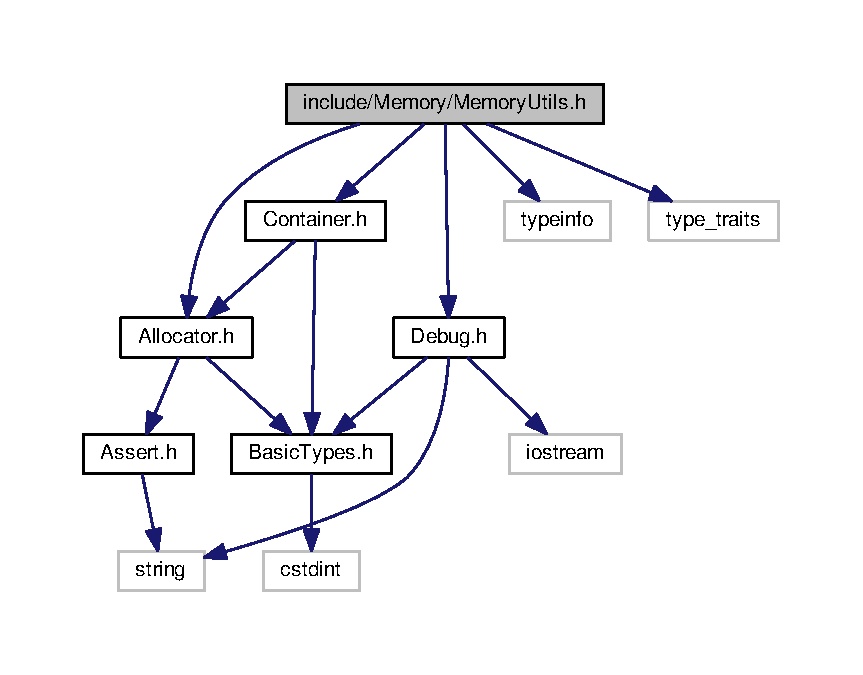
\includegraphics[width=350pt]{MemoryUtils_8h__incl}
\end{center}
\end{figure}
This graph shows which files directly or indirectly include this file\+:
\nopagebreak
\begin{figure}[H]
\begin{center}
\leavevmode
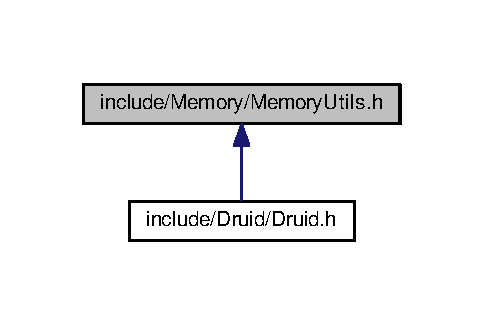
\includegraphics[width=232pt]{MemoryUtils_8h__dep__incl}
\end{center}
\end{figure}


\subsection{Detailed Description}
Functions for memory allocation. 


%--- End generated contents ---

% Index
\backmatter
\newpage
\phantomsection
\clearemptydoublepage
\addcontentsline{toc}{chapter}{Index}
\printindex

\end{document}
